\documentclass[english,a4paper]{article}
% Add support for UTF-8 character set for those engines that do not support it natively.
\usepackage[utf8]{inputenc}

% Consistent language in different packages, such as double quotes with \enquote and
% American-style hyphenation.
\usepackage[english]{babel}

% Handle multi-glyph charecters in the output PDF correctly
\usepackage[T1]{fontenc}

% Common math environments such as \begin{align}, and much, much more.
% Docs: http://texdoc.net/texmf-dist/doc/latex/amsmath/amsldoc.pdf
\usepackage{amsmath}

% Extended symbol collection
\usepackage{amssymb}

% Enhanced version of \newtheorem{}, which also allows non-numbered theorems.
\usepackage{amsthm}

% Add \od{}{} for ordinary derivatives, \pd{}{} for partial derivatives, and \del{} for delimiters.
% Docs: http://ctan.math.washington.edu/tex-archive/macros/latex/contrib/commath/commath.pdf
\usepackage{commath}

% Allows definition of colors using \definecolor{}{}{}
\usepackage{xcolor}

% For including source code with syntax highlighting.
% Docs: https://github.com/gpoore/minted/blob/master/source/minted.pdf
% newfloat disables loading of the float package, which is in conflict with floatrow
% See: https://tex.stackexchange.com/questions/378563/minted-and-floatrow-incompatible
\usepackage[newfloat]{minted}
% Enables the use of \begin{pythoncode}
\newminted{python}{python3=true}
% Enables the use of \begin{shellcode}
\definecolor{bgshell}{rgb}{0.95,0.95,0.95}
\newminted{shell}{bgcolor=bgshell,fontfamily=tt}

% Sitation management.
% Docs: http://ctan.uib.no/macros/latex/contrib/biblatex/doc/biblatex.pdf
% Tutorial: https://www.overleaf.com/learn/latex/Articles/Getting_started_with_BibLaTeX
\usepackage[style=numeric,backend=biber]{biblatex}
% Specify file containing all bibliographic metadata.
\addbibresource{bibliography.bib}

% Create figures with semantic code
\usepackage{tikz}
% Allow calculations within curly brackets in tikz figures
\usetikzlibrary{calc, math}
% Adds the braces decoration for showing distances in tikz figures
\usetikzlibrary{decorations.pathreplacing}
% For drawing matrices, useful for masking demonstration
\usetikzlibrary{matrix}

% Proper formatting of units by using \SI{value}{\unit}
% We enable use of \giga\byte and other binary units
\usepackage[binary-units=true]{siunitx}
\DeclareSIUnit\pixel{px}
\sisetup{range-phrase=~--~}

% For some reason, this package prevents some side-by-side tikz figures from wrapping
\usepackage[a4paper]{geometry}

% For insterting images into figures
\usepackage{graphicx}
\graphicspath{ {./img/} }

% Better formatting of URLs
\usepackage{url}

% Used for sectionsummary environment
\usepackage{tcolorbox}

% Wrap text around figures
\usepackage{wrapfig}

% Custom list formatting, such as noitemsep and label
\usepackage{enumitem}

% Nicer formatting of tables with \toprule, \midrule, and \bottomrule
\usepackage{booktabs}

% Enables the use of the subfigure environment for side-by-side figures
\usepackage{subcaption}

% Make figure captions dark gray
\definecolor{dark-gray}{gray}{0.25}
\usepackage[font={color=dark-gray},labelfont=bf]{caption}

% Good-looking inline fractions with \nicefrac{numerator}{denominator}
\usepackage{nicefrac}

% Correctly formatted quotation marks with \enquate{text}
\usepackage{csquotes}

% Used to position tables besides figures
\usepackage{floatrow}
\newfloatcommand{inlinetable}{table}[][\FBwidth]

% Defines the \vcentcolon symbol, used by the \defeq command
\usepackage{mathtools}

% Filler text with \blindtext and \Blindtext
\usepackage{blindtext}

% Fancy headers and footers
\usepackage{fancyhdr}

% Enables use of \pageref{LastPage} in header for "page x of y"-functionality
\usepackage{lastpage}

% Use \date{YYYY}{MM}{DD} in order to easily reformat dates at any time
\usepackage{datetime2}

% Better appendix functionality, such as separate headers and inclusion in TOC
\usepackage[toc,page]{appendix}

% Used by our custom "algorithm" environment
\usepackage{framed}

% --- General Configuration ---
\setlength{\parindent}{0em} % Indentation of beginning of paragraph
\setlength{\parskip}{0.5em} % Vertical space between paragraphs

% Allow fancyhdr package to reformat headers and footers
\pagestyle{fancy}

% Disable default header and footer
\fancyhf{}

% Add subsection name to upper left header
\fancyhead[L]{\footnotesize\rightmark}

% Remove horizontal line in header
\renewcommand{\headrulewidth}{0pt}

% Vector notation
\renewcommand{\vec}[1]{\boldsymbol{#1}}

% Expected value
\newcommand{\E}[1]{\mathrm{\mathb{E} \left[#1 \right]}}

% Variance
\newcommand{\Var}[1]{\mathrm{Var \left(#1 \right)}}

%  Summary of the intents of a given section
\newtcolorbox{sectionsummary}[0]{fonttitle=\bfseries,title=Section Summary}

% Used for coloring cadastrals
\definecolor{cadastralcolor}{rgb}{0,0,1}

% Colors used for confusions
\definecolor{tp}{HTML}{001F3F}
\definecolor{tn}{HTML}{DDDDDD}
\definecolor{fp}{HTML}{2ECC40}
\definecolor{fn}{HTML}{FF4136}


% Metadata for front page
\title{Building Footprint Detection Using Remote Sensing Data}
\author{Martinussen, Jakob Gerhard}
\date{Autumn, 2019}

\begin{document}
  \maketitle
  \thispagestyle{empty}  % Remove page number on title page
  \begin{abstract}
  We present a system for predicting building footprints by using remote sensing data in the form of aerial photography (RGB) and LiDAR elevation measurements (DSMs).
  Techniques for converting data from conventional GIS vector and raster formats to a format suitable for machine learning purposes are discussed.
  The U-Net model architecture is used in order to train several model variants on a labeled building footprint dataset covering the Norwegian municipality of Trondheim.
  A model using aerial photography in combination with LiDAR elevation data achieved the best mean IoU test score.
\end{abstract}
  % Abstract on title page
  \newpage
  \pagenumbering{roman} % Use roman numerals in first sections
  \fancyhead[R]{\footnotesize\thepage}  % Do not use page x of y, only x
  \tableofcontents
  \section{Image Segmentation --- Central Concepts and Previous Work}
We will now present our numerical experiments, using the theory presented in~\secref{sec:segmentation} and data produced by the pipeline outlined in~\secref{sec:data}.
Specifically the U-Net model architecture is used for segmentation as previously described in~\secref{sec:unet}.
We start by describing the general experimental setup in~\secref{sec:experimental-setup}.
A comparative investigation into the suitability of the different raster data types (aerial photography and/or LiDAR DSMs) for predicting building outlines is presented in~\secref{sec:features}.
In~\secref{sec:technique-experiments} we try to determine if techniques intended to combat overfitting and aid training actually have their intended effect; specifically batch normalization, dropout, and data augmentation.
The different LiDAR normalization methods presented in \algref{alg:local-min-max-scaling} and \algref{alg:metric-normalization} are implemented and compared in~\secref{sec:normalization-experiment}.
Finally, \secref{sec:loss-experiment} presents the empirical efficiency of different surrogate loss functions.


\subsection{Problem Description}%
\label{sec:segmentation-description}
Image recognition seeks to answer three questions for any given image~\cite{image_recognition}:

\begin{enumerate}[nosep]
  \item \textbf{Identification:} Does the image contain any object of interest?
  \item \textbf{Localization:} Where in the image are the objects situated?
  \item \textbf{Classification:} To which categories do the objects belong to?
\end{enumerate}

We will concern ourselves with only one object category (class) at any time, that class being building footprints, and will simplify the following theory accordingly with this simplification in mind.
The localization and classification of objects in a given image can be performed at different granularity levels, as shown in~\figref{fig:segmentation-types}.

\begin{figure}[htb]
  \includegraphics[width=\linewidth,trim={0 4cm 0 3.4cm},clip]{segmentation-types}
  \caption{
    Different granularities for single-class building localization, using the Trondheim 2017 data set.
    Bounding box regression is shown on the left, semantic segmentation in the middle, and instance segmentation on the right.
  }%
  \label{fig:segmentation-types}
\end{figure}
\newpage

\textit{Bounding box regression} concerns itself with finding the smallest possible rectangles which envelopes the objects of interest.
The sides of the rectangles may either by oriented parallel to the axis directions, or rotated in order to attain the smallest possible envelope.
The bounding box will therefore necessarily contain pixels that are not part of the object itself whenever the object shape is not perfectly rectangular.

\textit{Semantic segmentation} rectifies this issue by classifying each pixel in the image independently, i.e. \textit{pixel-wise} classification, producing a so-called classification \textit{mask}.
\textit{Instance segmentation} distinguishes between pixels belonging to different objects of the same class, while \textit{semantic segmentation} does not make this distinction.
Since a bounding box can be directly derived from a semantic segmentation mask, and a semantic segmentation mask can be directly derived from instance segmentation mask; the problem complexity of these tasks are as follows:
%
\begin{equation*}
  \text{Bounding box regression}
  <
  \text{Semantic segmentation}
  <
  \text{Instance segmentation}
\end{equation*}
%
An image of width $W$ and height $H$ consisting of $C$ channels is represented by a $W \times H \times C$ tensor, $X \in \mathbb{R}^{W \times H \times C}$.
This is somewhat simplified, but we will give a more nuanced description in~\secref{sec:raster-data}.
Single-class semantic segmentation can therefore be formalized as constructing a binary predictor $\tilde{f}$ of the form:
%
\begin{equation*}
  \tilde{f}: \mathbb{R}^{W \times H \times C} \rightarrow \mathbb{B}^{W \times H}, \hspace{2em} \mathbb{B} \defeq \{0, 1\}.
\end{equation*}
%
Where $\mathbb{B}^{W \times H}$ denotes a boolean matrix, $1$ indicating that the pixel is part of the object class of interest, and $0$ indicates the opposite.
In practice, however, statistical models will often predict a pixel-wise class \textit{confidence} in the continuous domain $[0, 1]$,
%
\begin{equation*}
  \hat{f}: \mathbb{R}^{W \times H \times C} \rightarrow {[0, 1]}^{W \times H},
\end{equation*}
%
but a binary predictor can be easily constructed by choosing a suitable threshold, $T$, for which to distinguish positive predictions from negative ones
%
\begin{equation*}
  \tilde{f}(X) = \hat{f}(X) > T, \hspace{2em} X \in \mathbb{R}^{W \times H \times C}.
\end{equation*}
%
The choice of the threshold value $T$ will affect the resulting \textit{sensitivity} and \textit{specificity} metrics of the model predictions, metrics which will be explained in the upcoming~\secref{sec:segmentation-metrics}.


\subsection{Convolutional Neural Networks (CNNs)}%
\label{sec:cnn}
  \topic{Convolution}
  As the name implies, a central concept of convolutional neural networks is the so-called \textit{convolution operator}.
Let the \textit{kernel}, $w$, be a $H_k \times W_k$ real matrix, and denote the activation of the previous layer at position $(x, y)$ as $a_{x, y}$.
The \textit{convolution operator}, $\circledast$, is then defined as
%
\begin{align*}
  w \circledast a_{x, y} = \sum_{i} \sum_{j} w_{i, j} ~ a_{x - i, y - j},
  \hspace{3em}
    a_{x, y} \in \mathbb{R},~
    w \in \mathbb{R}^{H_k \times W_k},
\end{align*}
%
where $(i, j)$ spans the index set of the kernel.
The region around $a_{x,y}$ which is involved in the convolution is referred to as the \textit{receptive field}.
We can generate a \textit{filtered image} by moving this receptive field over the entire input image.
The step size used when moving the receptive field is referred to as the \textit{stride size} of the convolution.
This \textit{moving convolution} is illustrated in \figref{fig:convolution}.

\begin{figure}[htb]
  As the name implies, a central concept of convolutional neural networks is the so-called \textit{convolution operator}.
Let the \textit{kernel}, $w$, be a $H_k \times W_k$ real matrix, and denote the activation of the previous layer at position $(x, y)$ as $a_{x, y}$.
The \textit{convolution operator}, $\circledast$, is then defined as
%
\begin{align*}
  w \circledast a_{x, y} = \sum_{i} \sum_{j} w_{i, j} ~ a_{x - i, y - j},
  \hspace{3em}
    a_{x, y} \in \mathbb{R},~
    w \in \mathbb{R}^{H_k \times W_k},
\end{align*}
%
where $(i, j)$ spans the index set of the kernel.
The region around $a_{x,y}$ which is involved in the convolution is referred to as the \textit{receptive field}.
We can generate a \textit{filtered image} by moving this receptive field over the entire input image.
The step size used when moving the receptive field is referred to as the \textit{stride size} of the convolution.
This \textit{moving convolution} is illustrated in \figref{fig:convolution}.

\begin{figure}[htb]
  \input{tikz/convolution.tex}
  \caption{
    Visualization of a kernel convolution with a $3 \times 3$ kernel over an image of size $4 \times 4$ with additional zero-padding and stride size $1$.
    The \textit{receptive field} is shown in \textcolor{orange}{orange}, the respective kernel weights in \textcolor{blue}{blue}, and the resulting convolution output in \textcolor{green}{green}.
    Zero padding of the input image is shown in gray.
  }
  \label{fig:convolution}
\end{figure}

\todo{Finish this section. Some ideas are given below.}

How should we interpret the kernel?
The concept of a \textit{kernel} predates neural networks, and is used in image processing.
Kernel convolution can result in reduction of dimensionality.
The first cause for dimension reduction is that the kernel $(n \times m)$ kernel matrix, with $n, m \geq 1$ can't possibly applied to a $N \times M$ image exactly $N \cdot M$ times. The convolution can't be fit into the image that many times.
We will therefore lose information on the edges of the image after having applied the convolution.
The solution to this problem is to pad the image with zeros.
There are other ways to reduce the dimensionality with convolution.
A $4 \times 4$ kernel with stride $4 \times 4$ will reduce the resolution in both dimensions by four, for instance.

  \caption{
    Visualization of a kernel convolution with a $3 \times 3$ kernel over an image of size $4 \times 4$ with additional zero-padding and stride size $1$.
    The \textit{receptive field} is shown in \textcolor{orange}{orange}, the respective kernel weights in \textcolor{blue}{blue}, and the resulting convolution output in \textcolor{green}{green}.
    Zero padding of the input image is shown in gray.
  }
  \label{fig:convolution}
\end{figure}

\todo{Finish this section. Some ideas are given below.}

How should we interpret the kernel?
The concept of a \textit{kernel} predates neural networks, and is used in image processing.
Kernel convolution can result in reduction of dimensionality.
The first cause for dimension reduction is that the kernel $(n \times m)$ kernel matrix, with $n, m \geq 1$ can't possibly applied to a $N \times M$ image exactly $N \cdot M$ times. The convolution can't be fit into the image that many times.
We will therefore lose information on the edges of the image after having applied the convolution.
The solution to this problem is to pad the image with zeros.
There are other ways to reduce the dimensionality with convolution.
A $4 \times 4$ kernel with stride $4 \times 4$ will reduce the resolution in both dimensions by four, for instance.

  \topic{Activation functions}
  So far we have only explained how a convolutional neural network consists of a set of parametrized linear combinations.
Such networks, if left unaltered, are therefore restricted to only approximating linear functions.
The solution to this predicament is to introduce the concept of \textit{activation functions}, a nonlinear function applied to the output of the convolutional layers.
These activation functions were originally inspired by the neuroscientific understanding of biological neurons~\cite[p.~165]{goodfellow}, but have also been shown to be a theoretical prerequisite of the \textit{universal approximation} property of artificial neural networks~\cite{uat-sigmoid,uat-nonpolynomial}.
The \textit{logistic sigmoid} function, with its deep roots in probability theory, has been a popular choice for activation function in neural networks since the inception of the field~\cite{rosenblatt-perceptron-1958}, and is defined by
%
\begin{equation*}
  \sigma(x) = \frac{1}{1 + e^{-x}} = \frac{e^x}{e^x + 1}.
  \tag{Sigmoid activation function}
\end{equation*}
%
Observe that $\lim_{x \to -\infty} \sigma(x) = 0$ and $\lim_{x \to +\infty} \sigma(x) = 1$, and that the derivative is positive over the entire real number line. This makes it a bounded, differentiable, monotonic function, and is therefore suitable for mapping the weighted output of an artificial neuron in the domain $(-\infty, \infty)$ into the range $(0, 1)$.
This makes it especially suitable for the final layer in neural networks intended for predicting binary 0/1-responses.

Although the sigmoid activation function has a strong biological~\cite{rosenblatt-perceptron-1958} and theoretical~\cite{uat-sigmoid} underpinning, it suffers from the phenomenon of \textit{vanishing gradients} for network architectures consisting of three or more layers, which severely inhibits training.
As an alternative to the sigmoid activation function, the \textit{rectified linear unit} (ReLU) was introduced in a paper~\cite{relu-original-paper} by \citeauthor{relu-original-paper} in year \citeyear{relu-original-paper}.
It is defined as
%
\begin{equation*}
  \mathrm{ReLU}(x) = x^+ = \max(0, x).
  \tag{ReLU activation function}
\end{equation*}
%
The ReLU activation function has become the dominant activation function for use in neural networks in recent years~\cite[p.~438]{relu-popularity} as it has been empirically shown to adapt better to deeper neural networks~\cite{relu-better-than-sigmoid}.

  \topic{Pooling}
  %%%%%%%%%%%%%%%%%%% Local functions %%%%%%%%%%%%%%%%%%%
%% -- Draw marks
\newbox\dumbox% chktex 1
\newcommand{\mymark}[2]{%
  \setbox\dumbox=\hbox{#2}%
  \hbox to \wd\dumbox{\hss% chktex 1
    \tikz[overlay,remember picture,baseline=(#1.base)]{\node (#1) {\box\dumbox};}% chktex 36
    \hss}%
}

%%%%%%%%%%%%%%%%%%% Local functions %%%%%%%%%%%%%%%%%%%

\[
\underbracket[0.6pt][7pt]{
\left[\begin{array}{cccc}
  1 & 8 & \mymark{TL1}{5} & \mymark{TR1}{0} \\
  8 & 11 & \mymark{BL1}{5} & \mymark{BR1}{4} \\
  8 & 17 &               10 & 11               \\
  9 & 12 & 10 & 7 \\
\end{array}\right]
}_{\text{Activations}}
\hspace{0.5em}
\underbracket[0.6pt][7pt]{
\begin{array}{ccc}
    \mymark{TL2}{\phantom{1}} & \phantom{1} & \mymark{TR2}{\phantom{1}}\\
    \phantom{1}  & \mymark{mycenter}{\phantom{1}} &              \phantom{0} \\
    \mymark{BL2}{\phantom{1}} & \phantom{0} & \mymark{BR2}{\phantom{0}}
\end{array}
}_{\text{Pool operation}}
=
\underbracket[0.6pt][7pt]{
\left[\begin{array}{cccccc}
  11 & \mymark{C}{5} \\
  17 & 11 \\
\end{array}\right]
}_{\text{Pooled output}}
\]

\begin{tikzpicture}[overlay, remember picture,
    myedge1/.style={thin, opacity=.3, blue},
    myedge2/.style={thin, opacity=.3, green!40!black}]

  %% Draw boxes
  \draw[orange, fill=orange, fill opacity=.1]   (TL1.north west) rectangle (BR1.south east);
  \draw[blue, fill=blue, fill opacity=.1] (TL2.north west) rectangle (BR2.south east)
    node[midway, opacity=1, color=black] {\Large $\max$};
  \draw[green!60!black, fill=green, fill opacity=.1] (C.north west) rectangle (C.south east);

  %% Draw blue lines
  \draw[myedge1] (TL1.north west) -- (TL2.north west);
  \draw[myedge1] (BL1.south west) -- (BL2.south west);
  \draw[myedge1] (TR1.north east) -- (TR2.north east);
  \draw[myedge1] (BR1.south east) -- (BR2.south east);

  %% Draw green lines
  \draw[myedge2] (TL2.north west) -- (C.north west);
  \draw[myedge2] (BL2.south west) -- (C.south west);
  \draw[myedge2] (TR2.north east) -- (C.north east);
  \draw[myedge2] (BR2.south east) -- (C.south east);
\end{tikzpicture}

  \topic{Batch normalization}
  The reparametrization of earlier layers when training deep neural networks results in a distributional change in the feature layer forwarded to the next layers.
This forces all subsequent layers to adapt to the new \enquote{distributional circumstances}, which in turn impedes the convergence of the optimization.
This phenomenon, referred to as \textit{internal covariate shift}, was first identified in a paper~\cite{batch-normalization} by \citeauthor{batch-normalization}~(\citeyear{batch-normalization}) where they propose a method called \textit{batch normalization} in order to counter this phenomenon.
Suppose we have a layer activation $\vec{a}$ consisting of $d$ dimensions, i.e. $\vec{a} = (a^{(1)}, \ldots, a^{(d)})$.
First we standardize each feature dimension, $k$, independently

\begin{equation*}
  \widehat{a}^{(k)}
  =
  \frac{
    a^{(k)} - \E{a^{(k)}}
  }{
    \sqrt{\Var{a^{(k)}} + \epsilon}
  },
  \tag{Batch standardization}
\end{equation*}

where $\E{\cdot}$ and $\Var{\cdot}$ are respectively sample means and sample variances over the current mini-batch, and $\epsilon$ is added for numerical stability.
The result of this standardization is a feature map where all filters have mean $0$ and variance $1$ for every mini-batch.
The internal covariate shift has been practically eliminated as a result.

This type of normalization alone may not be optimal in all cases, though, and is best explained by constructing a somewhat contrived pathological example.
Assume a set of pooled layer activations $\vec{a}$ to be symmetrically distributed, and assume the subsequent convolution layer to preserve this symmetry.
After standardizing the output, 50\% of the values are expected to be negative, and all of these values will be truncated to $0$ if ReLU is the activation function of choice.
This informational loss may be suboptimal for the given network layer and must be accounted for.
That is to say, $\E{a} =  0$ and $\Var{a}$ may be an unsuitable domain for the given activation function.
For this reason, we introduce two additional trainable parameters for each feature dimension, $\gamma^{(k)}$ and $\beta^{(k)}$, and apply a second normalization step

\begin{equation*}
  y^{(k)} = \gamma^{(k)} \widehat{a}^{(k)} + \beta^{(k)}.
  \tag{Trainable normalization}
\end{equation*}

The intent is to learn the values for the shift, $\beta^{(k)}$, and scaler, $\gamma^{(k)}$, which restores the representative power of the given layer \textit{after} the batch standardization.

  \topic{Dropout}
  Dropout is a regularization technique for neural networks intended to prevent \enquote{complex co-adaption of feature detectors}~\cite{dropout-original-paper}.
In practice this is achieved by randomly omitting hidden nodes from the neural network during each training step; effectively forcing hidden nodes to become less interdependent.
An alternative interpretation of the dropout procedure is that it is a computationally efficient form of model averaging, each dropout permutation being a single model instance.
This technique has been empirically shown to significantly increase the test performance in several different settings.

Although originally intended for use in feedforward neural networks, dropout has been extensively applied in CNN architectures as well~\cite{dropout-cnn}.
Since there are no nodes to be omitted in convolutional architectures, the dropout procedure needs to be adapted in order to be applicable in a CNN setting.
One approach is to introduce a randomly located square mask (\textit{cutout}) to the input image~\cite{dropout-cutout}.
\textit{Stochastic depth dropout} randomly selects entire layers to be dropped, replacing them with identity functions instead~\cite{dropout-stochastic-depth}.
Dropout can also be integrated into max pooling layers, ignoring values at random during the search for the maximum value in the receptive field~\cite{max-pooling-dropout}.
This has become known as \textit{max-pooling dropout} and is illustrated in~\figref{fig:max-pooling-dropout}.

\begin{figure}[htb]
  %%%%%%%%%%%%%%%%%%% Local functions %%%%%%%%%%%%%%%%%%%
%% -- Draw marks
\newbox\dumbox% chktex 1
\newcommand{\mymark}[2]{%
  \setbox\dumbox=\hbox{#2}%
  \hbox to \wd\dumbox{\hss% chktex 1
    \tikz[overlay,remember picture,baseline=(#1.base)]{\node (#1) {\box\dumbox};}% chktex 36
    \hss}%
}
% Used to indicate dropout array indices
\newcommand{\dropout}[1]{{\setlength{\fboxsep}{0pt}\fcolorbox{black}{black}{#1}}}

%%%%%%%%%%%%%%%%%%% Local functions %%%%%%%%%%%%%%%%%%%

\begin{align*}
  \left[\begin{array}{cccc}
    1 & 8 & \mymark{oldTL1}{5} & \mymark{oldTR1}{0} \\
    8 & 11 & \mymark{oldBL1}{5} & \mymark{oldBR1}{4} \\
    8 & 17 &               10 & 11               \\
    9 & \mymark{old}{12} & 10 & 7 \\
  \end{array}\right]
  \hspace{0.5em}
  \begin{array}{ccc}
      \mymark{oldTL2}{\phantom{1}} & \phantom{1} & \mymark{oldTR2}{\phantom{1}}\\
      \phantom{1}  & \mymark{oldmycenter}{\phantom{1}} &              \phantom{0} \\
      \mymark{oldBL2}{\phantom{1}} & \phantom{0} & \mymark{oldBR2}{\phantom{0}}
  \end{array}
  =
  \left[\begin{array}{cccccc}
    11 & \mymark{oldC}{5} \\
    17 & 11 \\
  \end{array}\right]
  \\[2.25em]
  \left[\begin{array}{cccc}
    1 & \mymark{new}{8} & \mymark{TL1}{\dropout{5}} & \mymark{TR1}{0} \\
    \dropout{8} & 11 & \mymark{BL1}{\dropout{5}} & \mymark{BR1}{4} \\
    8 & \dropout{1} &               10 & 11               \\
    \dropout{9} & 12 & 10 & 7 \\
  \end{array}\right]
  \hspace{0.5em}
  \begin{array}{ccc}
      \mymark{TL2}{\phantom{1}} & \phantom{1} & \mymark{TR2}{\phantom{1}}\\
      \phantom{1}  & \mymark{mycenter}{\phantom{1}} &              \phantom{0} \\
      \mymark{BL2}{\phantom{1}} & \phantom{0} & \mymark{BR2}{\phantom{0}}
  \end{array}
  =
  \left[\begin{array}{cccccc}
    11 & \mymark{C}{4} \\
    12 & 11 \\
  \end{array}\right]
\end{align*}

\begin{tikzpicture}[overlay, remember picture,
    myedge1/.style={thin, opacity=.3, blue},
    myedge2/.style={thin, opacity=.3, green!40!black}]

  %% Draw boxes
  \draw[orange, fill=orange, fill opacity=.1]   (TL1.north west) rectangle (BR1.south east);
  \draw[orange, fill=orange, fill opacity=.1]   (oldTL1.north west) rectangle (oldBR1.south east);

  \draw[blue, fill=blue, fill opacity=.1] (TL2.north west) rectangle (BR2.south east)
    node[midway, opacity=1, color=black] {\Large $\max$};
  \draw[blue, fill=blue, fill opacity=.1] (oldTL2.north west) rectangle (oldBR2.south east)
    node[midway, opacity=1, color=black] {\Large $\max$};

  \draw[green!60!black, fill=green, fill opacity=.1] (C.north west) rectangle (C.south east);
  \draw[green!60!black, fill=green, fill opacity=.1] (oldC.north west) rectangle (oldC.south east);

  %% Draw blue lines
  \draw[myedge1] (TL1.north west) -- (TL2.north west);
  \draw[myedge1] (BL1.south west) -- (BL2.south west);
  \draw[myedge1] (TR1.north east) -- (TR2.north east);
  \draw[myedge1] (BR1.south east) -- (BR2.south east);
  \draw[myedge1] (oldTL1.north west) -- (oldTL2.north west);
  \draw[myedge1] (oldBL1.south west) -- (oldBL2.south west);
  \draw[myedge1] (oldTR1.north east) -- (oldTR2.north east);
  \draw[myedge1] (oldBR1.south east) -- (oldBR2.south east);

  %% Draw green lines
  \draw[myedge2] (TL2.north west) -- (C.north west);
  \draw[myedge2] (BL2.south west) -- (C.south west);
  \draw[myedge2] (TR2.north east) -- (C.north east);
  \draw[myedge2] (BR2.south east) -- (C.south east);
  \draw[myedge2] (oldTL2.north west) -- (oldC.north west);
  \draw[myedge2] (oldBL2.south west) -- (oldC.south west);
  \draw[myedge2] (oldTR2.north east) -- (oldC.north east);
  \draw[myedge2] (oldBR2.south east) -- (oldC.south east);

  % Draw arrow from old to new activation matrix
  \draw[->, line width=0.5mm, shorten >= 2mm] (old) ++ (-0.1mm, -4mm) -- node[auto, yshift=1mm] {Dropout} (new.north);
\end{tikzpicture}

  \caption{%
    An example application of \textit{max-pooling dropout} using a receptive field and stride of size $2 \times 2$.
    A dropout probability of $p = 0.25$ has been used.
    Dropped values are shown as black boxes.
  }%
  \label{fig:max-pooling-dropout}
\end{figure}


\subsection{Metrics and Losses}%
\label{sec:segmentation-metrics}
We will now present our numerical experiments, using the theory presented in~\secref{sec:segmentation} and data produced by the pipeline outlined in~\secref{sec:data}.
Specifically the U-Net model architecture is used for segmentation as previously described in~\secref{sec:unet}.
We start by describing the general experimental setup in~\secref{sec:experimental-setup}.
A comparative investigation into the suitability of the different raster data types (aerial photography and/or LiDAR DSMs) for predicting building outlines is presented in~\secref{sec:features}.
In~\secref{sec:technique-experiments} we try to determine if techniques intended to combat overfitting and aid training actually have their intended effect; specifically batch normalization, dropout, and data augmentation.
The different LiDAR normalization methods presented in \algref{alg:local-min-max-scaling} and \algref{alg:metric-normalization} are implemented and compared in~\secref{sec:normalization-experiment}.
Finally, \secref{sec:loss-experiment} presents the empirical efficiency of different surrogate loss functions.

  \topic{Accuracy, sensitivity, and specificity}
  In order to describe segmentation metrics, it is useful to define the following quantities:

\begin{center}
  \fbox{
    \parbox{0.9\linewidth}{
      \begin{description}[font=\sffamily\bfseries, leftmargin=1cm]
        \item[Condition Positive (P)]
          Number of object class pixels in ground truth mask.
        \item[Condition Negative (N)]
          Number of non-object class pixels in ground truth mask.
        \item[True Positive (TP)]
          Number of pixels correctly predicted as being part of object class (correctly identified).
        \item[True Negative (TN)]
          Number of pixels correctly predicted as \textit{not} being part of object class (correctly rejected).
        \item[False Positive (FP)]
          Number of pixel incorrectly predicted as being part of object class (incorrectly identified).
        \item[False Negative (FN)]
          Number of pixel incorrectly predicted as \textit{not} being part of object class (incorrectly rejected).
      \end{description}
    }
  }
\end{center}

False positives (FP) are often knows as \textit{type I errors} in statistics, and false negatives (FN) as \textit{Type II errors}.
The greater the values of TP and TN, the better, and the smaller the values of FP and FN, the better.
A visual representation of these classifications is given in~\figref{fig:confusions}.

\begin{figure}[htb]
  \includegraphics[width=\linewidth]{confusions}
  \caption{
    Binary segmentation problem of size $256 \times 256$.
    The ground truth, a rectangle of size $120 \times 80$ is shown on the left.
    The \enquote{predicted} mask, shown in the middle, is of the same size, but offset by $(-30, -30)$.
    The right figure shows the visual equivalent of a confusion matrix.
    True positives are shown in \textcolor{tp}{dark blue}, true negatives in \textcolor{gray}{light gray}, false positives in \textcolor{fp}{green}, and false negatives in \textcolor{fn}{red}.
  }%
  \label{fig:confusions}
\end{figure}

The simplest metric for semantic segmentation is the \textit{pixel accuracy} metric.
This metric simply reports the percentage of pixels that were correctly classified.
More formally, it can be defined as:

\begin{equation*}
    \textbf{accuracy} = \frac{TP + TN}{TP + TN + FP + FN} = \frac{TP + TN}{P + N}
\end{equation*}

The problem with pixel-wise accuracy metrics is that it does not account for class imbalances.
Consider a problem where 95\% of all pixels are considered to be of class $0$, and the remaining 5\% of class $1$.
If we construct a model which predicts $0$ regardless of the feature inputs provided to the model, the model will achieve a 95\% accuracy score.
This makes pixel-wise accuracy scores difficult to interpret when you do not know the class balance of the respective dataset and the accuracy grouped by class.
This is why it is often replaced by other metrics which takes imbalances into account.
A pair of such metrics is \textit{sensitivity} and \textit{specificity}, formally defined as:

\begin{align*}
    \textbf{sensitivity}
    &=
    \frac{\text{number of true positives}}{\text{number of true positives + number of false negatives}}
    =
    \frac{TP}{TP + FN}
    =
    \frac{TP}{P}
    \\
    \textbf{specificity}
    &=
    \frac{\text{number of true negatives}}{\text{number of true negatives + number of false positives}}
    =
    \frac{TN}{TN + FP}
    =
    \frac{TN}{N}
\end{align*}

The \textit{sensitivity} is therefore a measure of how good the given model prediction was able to identify positives as a relative, fractional value.
Likewise, the \textit{specificity} is a measure of how good the given model prediction was able to identify negatives as a relative, fractional value.


  \topic{Intersection over union and dice coefficient}
  Although the sensitivity and specificity metrics address the issue of class imbalances, they are still \textit{two} distinct metrics that need to be simultaneously inspected in order to get a full performance picture of a given prediction.
We now pose the following problem: \enquote{is it possible to construct a \textit{single} scalar metric which incorporates the idea of sensitivity and specificity?}.
The \textit{intersection over union} (IoU) and \textit{dice coefficient} ($F_1$) are two attempts at solving this problem.

The IoU metric is defined as the area of the intersection between the predicted segmentation mask and the ground truth mask divided by the union of these two masks, or more formally
%
\begin{equation*}
  \mathrm{IoU}
  =
  \frac{%
    |\mathrm{prediction} \cap \mathrm{truth}|
  }{%
    |\mathrm{prediction} \cup \mathrm{truth}|
  }
  =
  \frac{%
    \mathrm{TP}
  }{%
    \mathrm{TP} + \mathrm{FP} + \mathrm{FN}
  }.
\end{equation*}
%
In the case of multiple classes IoU is calculated for each class independently and the result is averaged, known as \textit{mean intersection over union} (MIoU).
MIoU is the most commonly used segmentation metric in research and competitions due to its simplicity and representativeness~\cite{segmentation-overview}.
Notice how the IoU metric is bounded between 0 and 1; $\mathrm{IoU} = 0$ representing a complete \enquote{predictive miss} and $\mathrm{IoU} = 1$ representing a prediction in perfect accordance with the ground truth.
A visualization of this metric is given in \figref{fig:iou-metric} below.

\begin{figure}[H]
  \centering
  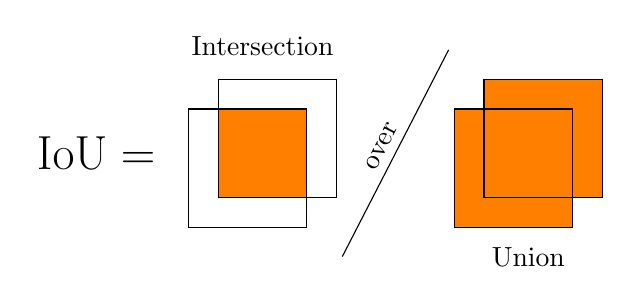
\begin{tikzpicture}[scale=0.75]
  \node[left] at (-0.4, 1.25) {\LARGE $\mathrm{IoU} = $};
  % Intersection illustration
  \begin{scope}
    \clip (0, 0) rectangle (2, 2);
    \fill[orange] (0.5, 0.5) rectangle (2.5, 2.5);
  \end{scope}
  \draw (0, 0) rectangle (2, 2);
  \draw (0.5, 0.5) rectangle (2.5, 2.5);
  \node[above, yshift=0.5em] at (1.25, 2.5) {Intersection};

  % Division sign
  \draw (2.6, -0.5) -- node[auto, sloped] {over} (4.4, 3);

  % Union illustration
  \begin{scope}[shift={(4.5, 0)}]
    \draw[fill=orange] (0, 0) rectangle (2, 2);
    \draw[fill=orange] (0.5, 0.5) rectangle (2.5, 2.5);
    \draw (0, 0) rectangle (2, 2);
    \node[below, yshift=-0.4em] at (1.25, 0) {Union};
  \end{scope}
\end{tikzpicture}

  \caption{%
    Visualization of single-class IoU metric.
  }%
  \label{fig:iou-metric}
\end{figure}

An alternative metric is the dice coefficient, often called the $F_1$ score as well.
The dice coefficient is defined by dividing twice the area of the intersection by the sum of the areas of the two masks:
%
\begin{equation*}
  \mathrm{F_1}
  =
  \frac{%
    2 \cdot |\mathrm{prediction} \cap \mathrm{truth}|
  }{%
    |\mathrm{prediction}| + |\mathrm{truth}|
  }
  =
  \frac{%
    \mathrm{2 \cdot TP}
  }{%
    2 \cdot \mathrm{TP} + \mathrm{FP} + \mathrm{FN}
  }.
\end{equation*}
%
Again we observe that this metric is bounded to the interval $[0, 1]$, with the same interpretation of the endpoints as with the IoU metric.
The visual representation of this metric is given in~\figref{fig:dice-coefficient}.

\begin{figure}[H]
  \centering
  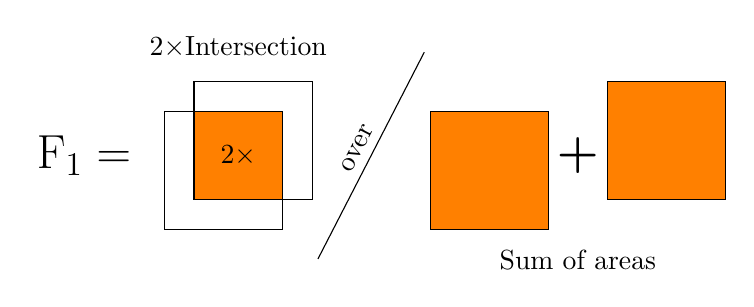
\begin{tikzpicture}[scale=0.75]
  \node[left] at (-0.4, 1.25) {\LARGE $\mathrm{F_1} = $};

  % Intersection illustration
  \begin{scope}
    \clip (0, 0) rectangle (2, 2);
    \fill[orange] (0.5, 0.5) rectangle (2.5, 2.5);
  \end{scope}
  \draw (0, 0) rectangle (2, 2);
  \draw (0.5, 0.5) rectangle (2.5, 2.5);
  \node[above, yshift=0.5em] at (1.25, 2.5) {$2 \times $Intersection};
  \node at (1.25, 1.25) {$2 \times$};

  % Division sign
  \draw (2.6, -0.5) -- node[auto, sloped] {over} (4.4, 3);

  % Union illustration
  \begin{scope}[shift={(4.5, 0)}]
    \draw[fill=orange] (0, 0) rectangle (2, 2);
    \begin{scope}[shift={(2.5, 0)}]
      \draw[fill=orange] (0.5, 0.5) rectangle (2.5, 2.5);
    \end{scope}
    \draw (0, 0) rectangle (2, 2);
    \node[below, yshift=-0.4em] at (2.5, 0) {Sum of areas};
    \node at (2.5, 1.25) {\LARGE \textbf{+}};
  \end{scope}
\end{tikzpicture}

  \caption{%
    Visualization of the single-class dice coefficient metric, also known as the $F_1$ score.
  }%
  \label{fig:dice-coefficient}
\end{figure}

You may have noticed that these two metrics are quite similar; they involve the same quantities, only weighted differently, and are bounded by to the same domain.
In fact, we can construct an exact relationship between these two metrics\footnote{The following relationship and the ensuing inequality bounds were noted by the \textit{Cross Validated Stack Exchange} user \enquote{Willem} here: \url{https://stats.stackexchange.com/a/276144}.}
%
\begin{equation*}
  \frac{%
    \mathrm{IoU}
  }{%
    \mathrm{F_1}
  }
  =
  \frac{1}{2}
  +
  \frac{%
    \mathrm{IoU}
  }{%
    2
  }.
\end{equation*}
%
The two metrics are therefore always positively correlated, as one metric increases or decreases, the other must necessarily follow suit.
A useful insight for how these two metrics actually differ is to observe how the IoU metric is bounded by the $\mathrm{F_1}$ metric:
%
\begin{equation*}
    \frac{%
      \mathrm{F_1}
    }{%
      2
    }
  \leq
    \mathrm{IoU}
  \leq
    \mathrm{F_1}
\end{equation*}
%
The IoU metric is \textit{always} less than or equal to the $\mathrm{F_1}$ metric, but never less than one half its value.
The fraction $\mathrm{IoU} / \mathrm{F_1}$ is equal to 1 whenever the prediction coincides with the ground truth and is equal to $1/2$ whenever there is no overlap at all.
By drawing an analogy to the $p = 1$ (absolute/Manhattan) norm and $p = 2$ (Euclidean) norm, the $\mathrm{IoU}$ metric is somewhat a reflection of the \textit{worst} performance, while the $\mathrm{F_1}$ metric is more a reflection of the \textit{average} performance of a given prediction.


  \topic{Binary cross-entropy and soft dice loss}
  So far all model experiments have been exclusively trained with the \textit{binary cross-entropy} loss function as given in equation~\eqref{eq:binary-cross-entropy}.
While this is the dominant loss function for binary classification tasks, it is still considered a suboptimal surrogate loss function for segmentation evaluation metrics such as the IoU metric.
Alternative loss functions were discussed in~\secref{sec:segmentation-metrics}, the so-called soft loss variants being of greatest interest.
Specifically, the \textit{soft Jaccard loss} given in equation~\eqref{eq:soft-jaccard-loss} and \textit{soft dice loss} given in equation~\eqref{eq:soft-dice-loss} having been theoretically and empirically shown to be efficient surrogate loss functions for the IoU metric.
Three models have been trained and evaluated, the only difference being which loss function that was used during training; binary cross-entropy, soft Jaccard loss, or soft dice loss.
The training procedures of these three models are visualized in \figref{fig:losses-training}.

\begin{figure}[H]
  \centering
  \includegraphics[width=0.66\linewidth]{metrics/lidar_dice_loss+lidar_jaccard_loss+without_rgb-validation-iou}
  \caption{%
    Three U-Net LiDAR models trained with different loss functions.
    Binary cross-entropy model shown in \textcolor{blue}{blue}, soft Jaccard in \textcolor{orange}{orange}, and soft dice shown in \textcolor{green}{green}.
  }%
  \label{fig:losses-training}
\end{figure}

The three models presented in~\figref{fig:losses-training} start out at approximately the same point after one epoch, but the binary cross-entropy model quickly outperforms the two other models when it comes to mean validation IoU.
The soft losses seem to be \emph{worse} surrogate losses for the IoU metric rather than better ones, completely contradicting our prior beliefs.

\begin{figure}[H]
  \centering
  \includegraphics[width=0.49\linewidth,trim={0 0.4cm 0 0.9cm},clip]{metric_correlation/without_rgb+lidar_jaccard_loss+iou}
  \textcolor{gray}{\vrule}
  \includegraphics[width=0.49\linewidth,trim={0 0.4cm 0 0.9cm},clip]{metric_correlation/without_rgb+lidar_dice_loss+iou}
  \caption{%
    Scatter plot showing the correlation between models using different losses during training.
    Both the left and right half of this figure compares model IoU against the binary cross-entropy IoU along the horizontal axis.
    Left figure half shows the soft Jaccard model on the vertical axis, while the right half shows the soft dice loss along the vertical axis.
    See caption of~\figref{fig:correlation-explanation} for detailed figure explanation.
  }
\end{figure}


\newpage
\subsection{State-of-the-Art}%
\label{sec:state-of-the-art}
We will give an overview of the current state of image segmentation.

\begin{itemize}
  \item Deep learning image segmentation overview given here~\cite{segmentation-overview} (\citeyear{segmentation-overview}).
  \item Recent semantic segmentation progress described here~\cite{segmentation-progress} (\citeyear{segmentation-progress}).
  \item Use of fully convolutional networks for semantic segmentation described here~\cite{segmentation-fcnn} (\citeyear{segmentation-fcnn}).
  \item SegNet architecture described here~\cite{segmentation-segnet} (\citeyear{segmentation-segnet}).
  \item U-Net architecture described here~\cite{segmentation-unet} (\citeyear{segmentation-unet}).
  \item Mask R-CNN architecture described here~\cite{segmentation-mask-r-cnn} (\citeyear{segmentation-mask-r-cnn}).
  \item SegCaps architecture described here~\cite{segmentation-segcaps} (\citeyear{segmentation-segcaps}).
  \item Panoptic feature pyramids described here~\cite{segmentation-panoptic-feature-pyramid} (\citeyear{segmentation-panoptic-feature-pyramid}).
\end{itemize}


  \section{Image Segmentation --- Central Concepts and Previous Work}
We will now present our numerical experiments, using the theory presented in~\secref{sec:segmentation} and data produced by the pipeline outlined in~\secref{sec:data}.
Specifically the U-Net model architecture is used for segmentation as previously described in~\secref{sec:unet}.
We start by describing the general experimental setup in~\secref{sec:experimental-setup}.
A comparative investigation into the suitability of the different raster data types (aerial photography and/or LiDAR DSMs) for predicting building outlines is presented in~\secref{sec:features}.
In~\secref{sec:technique-experiments} we try to determine if techniques intended to combat overfitting and aid training actually have their intended effect; specifically batch normalization, dropout, and data augmentation.
The different LiDAR normalization methods presented in \algref{alg:local-min-max-scaling} and \algref{alg:metric-normalization} are implemented and compared in~\secref{sec:normalization-experiment}.
Finally, \secref{sec:loss-experiment} presents the empirical efficiency of different surrogate loss functions.


\subsection{Problem Description}%
\label{sec:segmentation-description}
Image recognition seeks to answer three questions for any given image~\cite{image_recognition}:

\begin{enumerate}[nosep]
  \item \textbf{Identification:} Does the image contain any object of interest?
  \item \textbf{Localization:} Where in the image are the objects situated?
  \item \textbf{Classification:} To which categories do the objects belong to?
\end{enumerate}

We will concern ourselves with only one object category (class) at any time, that class being building footprints, and will simplify the following theory accordingly with this simplification in mind.
The localization and classification of objects in a given image can be performed at different granularity levels, as shown in~\figref{fig:segmentation-types}.

\begin{figure}[htb]
  \includegraphics[width=\linewidth,trim={0 4cm 0 3.4cm},clip]{segmentation-types}
  \caption{
    Different granularities for single-class building localization, using the Trondheim 2017 data set.
    Bounding box regression is shown on the left, semantic segmentation in the middle, and instance segmentation on the right.
  }%
  \label{fig:segmentation-types}
\end{figure}
\newpage

\textit{Bounding box regression} concerns itself with finding the smallest possible rectangles which envelopes the objects of interest.
The sides of the rectangles may either by oriented parallel to the axis directions, or rotated in order to attain the smallest possible envelope.
The bounding box will therefore necessarily contain pixels that are not part of the object itself whenever the object shape is not perfectly rectangular.

\textit{Semantic segmentation} rectifies this issue by classifying each pixel in the image independently, i.e. \textit{pixel-wise} classification, producing a so-called classification \textit{mask}.
\textit{Instance segmentation} distinguishes between pixels belonging to different objects of the same class, while \textit{semantic segmentation} does not make this distinction.
Since a bounding box can be directly derived from a semantic segmentation mask, and a semantic segmentation mask can be directly derived from instance segmentation mask; the problem complexity of these tasks are as follows:
%
\begin{equation*}
  \text{Bounding box regression}
  <
  \text{Semantic segmentation}
  <
  \text{Instance segmentation}
\end{equation*}
%
An image of width $W$ and height $H$ consisting of $C$ channels is represented by a $W \times H \times C$ tensor, $X \in \mathbb{R}^{W \times H \times C}$.
This is somewhat simplified, but we will give a more nuanced description in~\secref{sec:raster-data}.
Single-class semantic segmentation can therefore be formalized as constructing a binary predictor $\tilde{f}$ of the form:
%
\begin{equation*}
  \tilde{f}: \mathbb{R}^{W \times H \times C} \rightarrow \mathbb{B}^{W \times H}, \hspace{2em} \mathbb{B} \defeq \{0, 1\}.
\end{equation*}
%
Where $\mathbb{B}^{W \times H}$ denotes a boolean matrix, $1$ indicating that the pixel is part of the object class of interest, and $0$ indicates the opposite.
In practice, however, statistical models will often predict a pixel-wise class \textit{confidence} in the continuous domain $[0, 1]$,
%
\begin{equation*}
  \hat{f}: \mathbb{R}^{W \times H \times C} \rightarrow {[0, 1]}^{W \times H},
\end{equation*}
%
but a binary predictor can be easily constructed by choosing a suitable threshold, $T$, for which to distinguish positive predictions from negative ones
%
\begin{equation*}
  \tilde{f}(X) = \hat{f}(X) > T, \hspace{2em} X \in \mathbb{R}^{W \times H \times C}.
\end{equation*}
%
The choice of the threshold value $T$ will affect the resulting \textit{sensitivity} and \textit{specificity} metrics of the model predictions, metrics which will be explained in the upcoming~\secref{sec:segmentation-metrics}.


\subsection{Convolutional Neural Networks (CNNs)}%
\label{sec:cnn}
  \topic{Convolution}
  As the name implies, a central concept of convolutional neural networks is the so-called \textit{convolution operator}.
Let the \textit{kernel}, $w$, be a $H_k \times W_k$ real matrix, and denote the activation of the previous layer at position $(x, y)$ as $a_{x, y}$.
The \textit{convolution operator}, $\circledast$, is then defined as
%
\begin{align*}
  w \circledast a_{x, y} = \sum_{i} \sum_{j} w_{i, j} ~ a_{x - i, y - j},
  \hspace{3em}
    a_{x, y} \in \mathbb{R},~
    w \in \mathbb{R}^{H_k \times W_k},
\end{align*}
%
where $(i, j)$ spans the index set of the kernel.
The region around $a_{x,y}$ which is involved in the convolution is referred to as the \textit{receptive field}.
We can generate a \textit{filtered image} by moving this receptive field over the entire input image.
The step size used when moving the receptive field is referred to as the \textit{stride size} of the convolution.
This \textit{moving convolution} is illustrated in \figref{fig:convolution}.

\begin{figure}[htb]
  As the name implies, a central concept of convolutional neural networks is the so-called \textit{convolution operator}.
Let the \textit{kernel}, $w$, be a $H_k \times W_k$ real matrix, and denote the activation of the previous layer at position $(x, y)$ as $a_{x, y}$.
The \textit{convolution operator}, $\circledast$, is then defined as
%
\begin{align*}
  w \circledast a_{x, y} = \sum_{i} \sum_{j} w_{i, j} ~ a_{x - i, y - j},
  \hspace{3em}
    a_{x, y} \in \mathbb{R},~
    w \in \mathbb{R}^{H_k \times W_k},
\end{align*}
%
where $(i, j)$ spans the index set of the kernel.
The region around $a_{x,y}$ which is involved in the convolution is referred to as the \textit{receptive field}.
We can generate a \textit{filtered image} by moving this receptive field over the entire input image.
The step size used when moving the receptive field is referred to as the \textit{stride size} of the convolution.
This \textit{moving convolution} is illustrated in \figref{fig:convolution}.

\begin{figure}[htb]
  \input{tikz/convolution.tex}
  \caption{
    Visualization of a kernel convolution with a $3 \times 3$ kernel over an image of size $4 \times 4$ with additional zero-padding and stride size $1$.
    The \textit{receptive field} is shown in \textcolor{orange}{orange}, the respective kernel weights in \textcolor{blue}{blue}, and the resulting convolution output in \textcolor{green}{green}.
    Zero padding of the input image is shown in gray.
  }
  \label{fig:convolution}
\end{figure}

\todo{Finish this section. Some ideas are given below.}

How should we interpret the kernel?
The concept of a \textit{kernel} predates neural networks, and is used in image processing.
Kernel convolution can result in reduction of dimensionality.
The first cause for dimension reduction is that the kernel $(n \times m)$ kernel matrix, with $n, m \geq 1$ can't possibly applied to a $N \times M$ image exactly $N \cdot M$ times. The convolution can't be fit into the image that many times.
We will therefore lose information on the edges of the image after having applied the convolution.
The solution to this problem is to pad the image with zeros.
There are other ways to reduce the dimensionality with convolution.
A $4 \times 4$ kernel with stride $4 \times 4$ will reduce the resolution in both dimensions by four, for instance.

  \caption{
    Visualization of a kernel convolution with a $3 \times 3$ kernel over an image of size $4 \times 4$ with additional zero-padding and stride size $1$.
    The \textit{receptive field} is shown in \textcolor{orange}{orange}, the respective kernel weights in \textcolor{blue}{blue}, and the resulting convolution output in \textcolor{green}{green}.
    Zero padding of the input image is shown in gray.
  }
  \label{fig:convolution}
\end{figure}

\todo{Finish this section. Some ideas are given below.}

How should we interpret the kernel?
The concept of a \textit{kernel} predates neural networks, and is used in image processing.
Kernel convolution can result in reduction of dimensionality.
The first cause for dimension reduction is that the kernel $(n \times m)$ kernel matrix, with $n, m \geq 1$ can't possibly applied to a $N \times M$ image exactly $N \cdot M$ times. The convolution can't be fit into the image that many times.
We will therefore lose information on the edges of the image after having applied the convolution.
The solution to this problem is to pad the image with zeros.
There are other ways to reduce the dimensionality with convolution.
A $4 \times 4$ kernel with stride $4 \times 4$ will reduce the resolution in both dimensions by four, for instance.

  \topic{Activation functions}
  So far we have only explained how a convolutional neural network consists of a set of parametrized linear combinations.
Such networks, if left unaltered, are therefore restricted to only approximating linear functions.
The solution to this predicament is to introduce the concept of \textit{activation functions}, a nonlinear function applied to the output of the convolutional layers.
These activation functions were originally inspired by the neuroscientific understanding of biological neurons~\cite[p.~165]{goodfellow}, but have also been shown to be a theoretical prerequisite of the \textit{universal approximation} property of artificial neural networks~\cite{uat-sigmoid,uat-nonpolynomial}.
The \textit{logistic sigmoid} function, with its deep roots in probability theory, has been a popular choice for activation function in neural networks since the inception of the field~\cite{rosenblatt-perceptron-1958}, and is defined by
%
\begin{equation*}
  \sigma(x) = \frac{1}{1 + e^{-x}} = \frac{e^x}{e^x + 1}.
  \tag{Sigmoid activation function}
\end{equation*}
%
Observe that $\lim_{x \to -\infty} \sigma(x) = 0$ and $\lim_{x \to +\infty} \sigma(x) = 1$, and that the derivative is positive over the entire real number line. This makes it a bounded, differentiable, monotonic function, and is therefore suitable for mapping the weighted output of an artificial neuron in the domain $(-\infty, \infty)$ into the range $(0, 1)$.
This makes it especially suitable for the final layer in neural networks intended for predicting binary 0/1-responses.

Although the sigmoid activation function has a strong biological~\cite{rosenblatt-perceptron-1958} and theoretical~\cite{uat-sigmoid} underpinning, it suffers from the phenomenon of \textit{vanishing gradients} for network architectures consisting of three or more layers, which severely inhibits training.
As an alternative to the sigmoid activation function, the \textit{rectified linear unit} (ReLU) was introduced in a paper~\cite{relu-original-paper} by \citeauthor{relu-original-paper} in year \citeyear{relu-original-paper}.
It is defined as
%
\begin{equation*}
  \mathrm{ReLU}(x) = x^+ = \max(0, x).
  \tag{ReLU activation function}
\end{equation*}
%
The ReLU activation function has become the dominant activation function for use in neural networks in recent years~\cite[p.~438]{relu-popularity} as it has been empirically shown to adapt better to deeper neural networks~\cite{relu-better-than-sigmoid}.

  \topic{Pooling}
  %%%%%%%%%%%%%%%%%%% Local functions %%%%%%%%%%%%%%%%%%%
%% -- Draw marks
\newbox\dumbox% chktex 1
\newcommand{\mymark}[2]{%
  \setbox\dumbox=\hbox{#2}%
  \hbox to \wd\dumbox{\hss% chktex 1
    \tikz[overlay,remember picture,baseline=(#1.base)]{\node (#1) {\box\dumbox};}% chktex 36
    \hss}%
}

%%%%%%%%%%%%%%%%%%% Local functions %%%%%%%%%%%%%%%%%%%

\[
\underbracket[0.6pt][7pt]{
\left[\begin{array}{cccc}
  1 & 8 & \mymark{TL1}{5} & \mymark{TR1}{0} \\
  8 & 11 & \mymark{BL1}{5} & \mymark{BR1}{4} \\
  8 & 17 &               10 & 11               \\
  9 & 12 & 10 & 7 \\
\end{array}\right]
}_{\text{Activations}}
\hspace{0.5em}
\underbracket[0.6pt][7pt]{
\begin{array}{ccc}
    \mymark{TL2}{\phantom{1}} & \phantom{1} & \mymark{TR2}{\phantom{1}}\\
    \phantom{1}  & \mymark{mycenter}{\phantom{1}} &              \phantom{0} \\
    \mymark{BL2}{\phantom{1}} & \phantom{0} & \mymark{BR2}{\phantom{0}}
\end{array}
}_{\text{Pool operation}}
=
\underbracket[0.6pt][7pt]{
\left[\begin{array}{cccccc}
  11 & \mymark{C}{5} \\
  17 & 11 \\
\end{array}\right]
}_{\text{Pooled output}}
\]

\begin{tikzpicture}[overlay, remember picture,
    myedge1/.style={thin, opacity=.3, blue},
    myedge2/.style={thin, opacity=.3, green!40!black}]

  %% Draw boxes
  \draw[orange, fill=orange, fill opacity=.1]   (TL1.north west) rectangle (BR1.south east);
  \draw[blue, fill=blue, fill opacity=.1] (TL2.north west) rectangle (BR2.south east)
    node[midway, opacity=1, color=black] {\Large $\max$};
  \draw[green!60!black, fill=green, fill opacity=.1] (C.north west) rectangle (C.south east);

  %% Draw blue lines
  \draw[myedge1] (TL1.north west) -- (TL2.north west);
  \draw[myedge1] (BL1.south west) -- (BL2.south west);
  \draw[myedge1] (TR1.north east) -- (TR2.north east);
  \draw[myedge1] (BR1.south east) -- (BR2.south east);

  %% Draw green lines
  \draw[myedge2] (TL2.north west) -- (C.north west);
  \draw[myedge2] (BL2.south west) -- (C.south west);
  \draw[myedge2] (TR2.north east) -- (C.north east);
  \draw[myedge2] (BR2.south east) -- (C.south east);
\end{tikzpicture}

  \topic{Batch normalization}
  The reparametrization of earlier layers when training deep neural networks results in a distributional change in the feature layer forwarded to the next layers.
This forces all subsequent layers to adapt to the new \enquote{distributional circumstances}, which in turn impedes the convergence of the optimization.
This phenomenon, referred to as \textit{internal covariate shift}, was first identified in a paper~\cite{batch-normalization} by \citeauthor{batch-normalization}~(\citeyear{batch-normalization}) where they propose a method called \textit{batch normalization} in order to counter this phenomenon.
Suppose we have a layer activation $\vec{a}$ consisting of $d$ dimensions, i.e. $\vec{a} = (a^{(1)}, \ldots, a^{(d)})$.
First we standardize each feature dimension, $k$, independently

\begin{equation*}
  \widehat{a}^{(k)}
  =
  \frac{
    a^{(k)} - \E{a^{(k)}}
  }{
    \sqrt{\Var{a^{(k)}} + \epsilon}
  },
  \tag{Batch standardization}
\end{equation*}

where $\E{\cdot}$ and $\Var{\cdot}$ are respectively sample means and sample variances over the current mini-batch, and $\epsilon$ is added for numerical stability.
The result of this standardization is a feature map where all filters have mean $0$ and variance $1$ for every mini-batch.
The internal covariate shift has been practically eliminated as a result.

This type of normalization alone may not be optimal in all cases, though, and is best explained by constructing a somewhat contrived pathological example.
Assume a set of pooled layer activations $\vec{a}$ to be symmetrically distributed, and assume the subsequent convolution layer to preserve this symmetry.
After standardizing the output, 50\% of the values are expected to be negative, and all of these values will be truncated to $0$ if ReLU is the activation function of choice.
This informational loss may be suboptimal for the given network layer and must be accounted for.
That is to say, $\E{a} =  0$ and $\Var{a}$ may be an unsuitable domain for the given activation function.
For this reason, we introduce two additional trainable parameters for each feature dimension, $\gamma^{(k)}$ and $\beta^{(k)}$, and apply a second normalization step

\begin{equation*}
  y^{(k)} = \gamma^{(k)} \widehat{a}^{(k)} + \beta^{(k)}.
  \tag{Trainable normalization}
\end{equation*}

The intent is to learn the values for the shift, $\beta^{(k)}$, and scaler, $\gamma^{(k)}$, which restores the representative power of the given layer \textit{after} the batch standardization.

  \topic{Dropout}
  Dropout is a regularization technique for neural networks intended to prevent \enquote{complex co-adaption of feature detectors}~\cite{dropout-original-paper}.
In practice this is achieved by randomly omitting hidden nodes from the neural network during each training step; effectively forcing hidden nodes to become less interdependent.
An alternative interpretation of the dropout procedure is that it is a computationally efficient form of model averaging, each dropout permutation being a single model instance.
This technique has been empirically shown to significantly increase the test performance in several different settings.

Although originally intended for use in feedforward neural networks, dropout has been extensively applied in CNN architectures as well~\cite{dropout-cnn}.
Since there are no nodes to be omitted in convolutional architectures, the dropout procedure needs to be adapted in order to be applicable in a CNN setting.
One approach is to introduce a randomly located square mask (\textit{cutout}) to the input image~\cite{dropout-cutout}.
\textit{Stochastic depth dropout} randomly selects entire layers to be dropped, replacing them with identity functions instead~\cite{dropout-stochastic-depth}.
Dropout can also be integrated into max pooling layers, ignoring values at random during the search for the maximum value in the receptive field~\cite{max-pooling-dropout}.
This has become known as \textit{max-pooling dropout} and is illustrated in~\figref{fig:max-pooling-dropout}.

\begin{figure}[htb]
  %%%%%%%%%%%%%%%%%%% Local functions %%%%%%%%%%%%%%%%%%%
%% -- Draw marks
\newbox\dumbox% chktex 1
\newcommand{\mymark}[2]{%
  \setbox\dumbox=\hbox{#2}%
  \hbox to \wd\dumbox{\hss% chktex 1
    \tikz[overlay,remember picture,baseline=(#1.base)]{\node (#1) {\box\dumbox};}% chktex 36
    \hss}%
}
% Used to indicate dropout array indices
\newcommand{\dropout}[1]{{\setlength{\fboxsep}{0pt}\fcolorbox{black}{black}{#1}}}

%%%%%%%%%%%%%%%%%%% Local functions %%%%%%%%%%%%%%%%%%%

\begin{align*}
  \left[\begin{array}{cccc}
    1 & 8 & \mymark{oldTL1}{5} & \mymark{oldTR1}{0} \\
    8 & 11 & \mymark{oldBL1}{5} & \mymark{oldBR1}{4} \\
    8 & 17 &               10 & 11               \\
    9 & \mymark{old}{12} & 10 & 7 \\
  \end{array}\right]
  \hspace{0.5em}
  \begin{array}{ccc}
      \mymark{oldTL2}{\phantom{1}} & \phantom{1} & \mymark{oldTR2}{\phantom{1}}\\
      \phantom{1}  & \mymark{oldmycenter}{\phantom{1}} &              \phantom{0} \\
      \mymark{oldBL2}{\phantom{1}} & \phantom{0} & \mymark{oldBR2}{\phantom{0}}
  \end{array}
  =
  \left[\begin{array}{cccccc}
    11 & \mymark{oldC}{5} \\
    17 & 11 \\
  \end{array}\right]
  \\[2.25em]
  \left[\begin{array}{cccc}
    1 & \mymark{new}{8} & \mymark{TL1}{\dropout{5}} & \mymark{TR1}{0} \\
    \dropout{8} & 11 & \mymark{BL1}{\dropout{5}} & \mymark{BR1}{4} \\
    8 & \dropout{1} &               10 & 11               \\
    \dropout{9} & 12 & 10 & 7 \\
  \end{array}\right]
  \hspace{0.5em}
  \begin{array}{ccc}
      \mymark{TL2}{\phantom{1}} & \phantom{1} & \mymark{TR2}{\phantom{1}}\\
      \phantom{1}  & \mymark{mycenter}{\phantom{1}} &              \phantom{0} \\
      \mymark{BL2}{\phantom{1}} & \phantom{0} & \mymark{BR2}{\phantom{0}}
  \end{array}
  =
  \left[\begin{array}{cccccc}
    11 & \mymark{C}{4} \\
    12 & 11 \\
  \end{array}\right]
\end{align*}

\begin{tikzpicture}[overlay, remember picture,
    myedge1/.style={thin, opacity=.3, blue},
    myedge2/.style={thin, opacity=.3, green!40!black}]

  %% Draw boxes
  \draw[orange, fill=orange, fill opacity=.1]   (TL1.north west) rectangle (BR1.south east);
  \draw[orange, fill=orange, fill opacity=.1]   (oldTL1.north west) rectangle (oldBR1.south east);

  \draw[blue, fill=blue, fill opacity=.1] (TL2.north west) rectangle (BR2.south east)
    node[midway, opacity=1, color=black] {\Large $\max$};
  \draw[blue, fill=blue, fill opacity=.1] (oldTL2.north west) rectangle (oldBR2.south east)
    node[midway, opacity=1, color=black] {\Large $\max$};

  \draw[green!60!black, fill=green, fill opacity=.1] (C.north west) rectangle (C.south east);
  \draw[green!60!black, fill=green, fill opacity=.1] (oldC.north west) rectangle (oldC.south east);

  %% Draw blue lines
  \draw[myedge1] (TL1.north west) -- (TL2.north west);
  \draw[myedge1] (BL1.south west) -- (BL2.south west);
  \draw[myedge1] (TR1.north east) -- (TR2.north east);
  \draw[myedge1] (BR1.south east) -- (BR2.south east);
  \draw[myedge1] (oldTL1.north west) -- (oldTL2.north west);
  \draw[myedge1] (oldBL1.south west) -- (oldBL2.south west);
  \draw[myedge1] (oldTR1.north east) -- (oldTR2.north east);
  \draw[myedge1] (oldBR1.south east) -- (oldBR2.south east);

  %% Draw green lines
  \draw[myedge2] (TL2.north west) -- (C.north west);
  \draw[myedge2] (BL2.south west) -- (C.south west);
  \draw[myedge2] (TR2.north east) -- (C.north east);
  \draw[myedge2] (BR2.south east) -- (C.south east);
  \draw[myedge2] (oldTL2.north west) -- (oldC.north west);
  \draw[myedge2] (oldBL2.south west) -- (oldC.south west);
  \draw[myedge2] (oldTR2.north east) -- (oldC.north east);
  \draw[myedge2] (oldBR2.south east) -- (oldC.south east);

  % Draw arrow from old to new activation matrix
  \draw[->, line width=0.5mm, shorten >= 2mm] (old) ++ (-0.1mm, -4mm) -- node[auto, yshift=1mm] {Dropout} (new.north);
\end{tikzpicture}

  \caption{%
    An example application of \textit{max-pooling dropout} using a receptive field and stride of size $2 \times 2$.
    A dropout probability of $p = 0.25$ has been used.
    Dropped values are shown as black boxes.
  }%
  \label{fig:max-pooling-dropout}
\end{figure}


\subsection{Metrics and Losses}%
\label{sec:segmentation-metrics}
We will now present our numerical experiments, using the theory presented in~\secref{sec:segmentation} and data produced by the pipeline outlined in~\secref{sec:data}.
Specifically the U-Net model architecture is used for segmentation as previously described in~\secref{sec:unet}.
We start by describing the general experimental setup in~\secref{sec:experimental-setup}.
A comparative investigation into the suitability of the different raster data types (aerial photography and/or LiDAR DSMs) for predicting building outlines is presented in~\secref{sec:features}.
In~\secref{sec:technique-experiments} we try to determine if techniques intended to combat overfitting and aid training actually have their intended effect; specifically batch normalization, dropout, and data augmentation.
The different LiDAR normalization methods presented in \algref{alg:local-min-max-scaling} and \algref{alg:metric-normalization} are implemented and compared in~\secref{sec:normalization-experiment}.
Finally, \secref{sec:loss-experiment} presents the empirical efficiency of different surrogate loss functions.

  \topic{Accuracy, sensitivity, and specificity}
  In order to describe segmentation metrics, it is useful to define the following quantities:

\begin{center}
  \fbox{
    \parbox{0.9\linewidth}{
      \begin{description}[font=\sffamily\bfseries, leftmargin=1cm]
        \item[Condition Positive (P)]
          Number of object class pixels in ground truth mask.
        \item[Condition Negative (N)]
          Number of non-object class pixels in ground truth mask.
        \item[True Positive (TP)]
          Number of pixels correctly predicted as being part of object class (correctly identified).
        \item[True Negative (TN)]
          Number of pixels correctly predicted as \textit{not} being part of object class (correctly rejected).
        \item[False Positive (FP)]
          Number of pixel incorrectly predicted as being part of object class (incorrectly identified).
        \item[False Negative (FN)]
          Number of pixel incorrectly predicted as \textit{not} being part of object class (incorrectly rejected).
      \end{description}
    }
  }
\end{center}

False positives (FP) are often knows as \textit{type I errors} in statistics, and false negatives (FN) as \textit{Type II errors}.
The greater the values of TP and TN, the better, and the smaller the values of FP and FN, the better.
A visual representation of these classifications is given in~\figref{fig:confusions}.

\begin{figure}[htb]
  \includegraphics[width=\linewidth]{confusions}
  \caption{
    Binary segmentation problem of size $256 \times 256$.
    The ground truth, a rectangle of size $120 \times 80$ is shown on the left.
    The \enquote{predicted} mask, shown in the middle, is of the same size, but offset by $(-30, -30)$.
    The right figure shows the visual equivalent of a confusion matrix.
    True positives are shown in \textcolor{tp}{dark blue}, true negatives in \textcolor{gray}{light gray}, false positives in \textcolor{fp}{green}, and false negatives in \textcolor{fn}{red}.
  }%
  \label{fig:confusions}
\end{figure}

The simplest metric for semantic segmentation is the \textit{pixel accuracy} metric.
This metric simply reports the percentage of pixels that were correctly classified.
More formally, it can be defined as:

\begin{equation*}
    \textbf{accuracy} = \frac{TP + TN}{TP + TN + FP + FN} = \frac{TP + TN}{P + N}
\end{equation*}

The problem with pixel-wise accuracy metrics is that it does not account for class imbalances.
Consider a problem where 95\% of all pixels are considered to be of class $0$, and the remaining 5\% of class $1$.
If we construct a model which predicts $0$ regardless of the feature inputs provided to the model, the model will achieve a 95\% accuracy score.
This makes pixel-wise accuracy scores difficult to interpret when you do not know the class balance of the respective dataset and the accuracy grouped by class.
This is why it is often replaced by other metrics which takes imbalances into account.
A pair of such metrics is \textit{sensitivity} and \textit{specificity}, formally defined as:

\begin{align*}
    \textbf{sensitivity}
    &=
    \frac{\text{number of true positives}}{\text{number of true positives + number of false negatives}}
    =
    \frac{TP}{TP + FN}
    =
    \frac{TP}{P}
    \\
    \textbf{specificity}
    &=
    \frac{\text{number of true negatives}}{\text{number of true negatives + number of false positives}}
    =
    \frac{TN}{TN + FP}
    =
    \frac{TN}{N}
\end{align*}

The \textit{sensitivity} is therefore a measure of how good the given model prediction was able to identify positives as a relative, fractional value.
Likewise, the \textit{specificity} is a measure of how good the given model prediction was able to identify negatives as a relative, fractional value.


  \topic{Intersection over union and dice coefficient}
  Although the sensitivity and specificity metrics address the issue of class imbalances, they are still \textit{two} distinct metrics that need to be simultaneously inspected in order to get a full performance picture of a given prediction.
We now pose the following problem: \enquote{is it possible to construct a \textit{single} scalar metric which incorporates the idea of sensitivity and specificity?}.
The \textit{intersection over union} (IoU) and \textit{dice coefficient} ($F_1$) are two attempts at solving this problem.

The IoU metric is defined as the area of the intersection between the predicted segmentation mask and the ground truth mask divided by the union of these two masks, or more formally
%
\begin{equation*}
  \mathrm{IoU}
  =
  \frac{%
    |\mathrm{prediction} \cap \mathrm{truth}|
  }{%
    |\mathrm{prediction} \cup \mathrm{truth}|
  }
  =
  \frac{%
    \mathrm{TP}
  }{%
    \mathrm{TP} + \mathrm{FP} + \mathrm{FN}
  }.
\end{equation*}
%
In the case of multiple classes IoU is calculated for each class independently and the result is averaged, known as \textit{mean intersection over union} (MIoU).
MIoU is the most commonly used segmentation metric in research and competitions due to its simplicity and representativeness~\cite{segmentation-overview}.
Notice how the IoU metric is bounded between 0 and 1; $\mathrm{IoU} = 0$ representing a complete \enquote{predictive miss} and $\mathrm{IoU} = 1$ representing a prediction in perfect accordance with the ground truth.
A visualization of this metric is given in \figref{fig:iou-metric} below.

\begin{figure}[H]
  \centering
  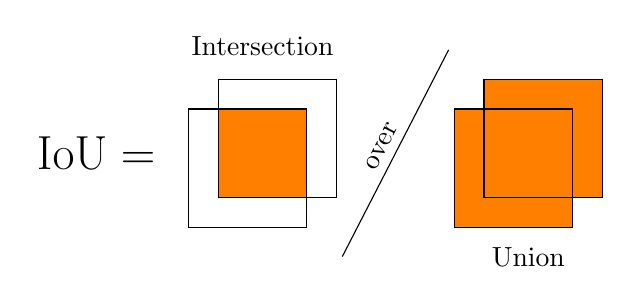
\begin{tikzpicture}[scale=0.75]
  \node[left] at (-0.4, 1.25) {\LARGE $\mathrm{IoU} = $};
  % Intersection illustration
  \begin{scope}
    \clip (0, 0) rectangle (2, 2);
    \fill[orange] (0.5, 0.5) rectangle (2.5, 2.5);
  \end{scope}
  \draw (0, 0) rectangle (2, 2);
  \draw (0.5, 0.5) rectangle (2.5, 2.5);
  \node[above, yshift=0.5em] at (1.25, 2.5) {Intersection};

  % Division sign
  \draw (2.6, -0.5) -- node[auto, sloped] {over} (4.4, 3);

  % Union illustration
  \begin{scope}[shift={(4.5, 0)}]
    \draw[fill=orange] (0, 0) rectangle (2, 2);
    \draw[fill=orange] (0.5, 0.5) rectangle (2.5, 2.5);
    \draw (0, 0) rectangle (2, 2);
    \node[below, yshift=-0.4em] at (1.25, 0) {Union};
  \end{scope}
\end{tikzpicture}

  \caption{%
    Visualization of single-class IoU metric.
  }%
  \label{fig:iou-metric}
\end{figure}

An alternative metric is the dice coefficient, often called the $F_1$ score as well.
The dice coefficient is defined by dividing twice the area of the intersection by the sum of the areas of the two masks:
%
\begin{equation*}
  \mathrm{F_1}
  =
  \frac{%
    2 \cdot |\mathrm{prediction} \cap \mathrm{truth}|
  }{%
    |\mathrm{prediction}| + |\mathrm{truth}|
  }
  =
  \frac{%
    \mathrm{2 \cdot TP}
  }{%
    2 \cdot \mathrm{TP} + \mathrm{FP} + \mathrm{FN}
  }.
\end{equation*}
%
Again we observe that this metric is bounded to the interval $[0, 1]$, with the same interpretation of the endpoints as with the IoU metric.
The visual representation of this metric is given in~\figref{fig:dice-coefficient}.

\begin{figure}[H]
  \centering
  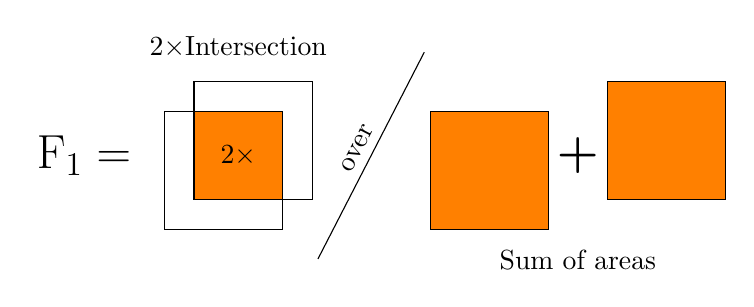
\begin{tikzpicture}[scale=0.75]
  \node[left] at (-0.4, 1.25) {\LARGE $\mathrm{F_1} = $};

  % Intersection illustration
  \begin{scope}
    \clip (0, 0) rectangle (2, 2);
    \fill[orange] (0.5, 0.5) rectangle (2.5, 2.5);
  \end{scope}
  \draw (0, 0) rectangle (2, 2);
  \draw (0.5, 0.5) rectangle (2.5, 2.5);
  \node[above, yshift=0.5em] at (1.25, 2.5) {$2 \times $Intersection};
  \node at (1.25, 1.25) {$2 \times$};

  % Division sign
  \draw (2.6, -0.5) -- node[auto, sloped] {over} (4.4, 3);

  % Union illustration
  \begin{scope}[shift={(4.5, 0)}]
    \draw[fill=orange] (0, 0) rectangle (2, 2);
    \begin{scope}[shift={(2.5, 0)}]
      \draw[fill=orange] (0.5, 0.5) rectangle (2.5, 2.5);
    \end{scope}
    \draw (0, 0) rectangle (2, 2);
    \node[below, yshift=-0.4em] at (2.5, 0) {Sum of areas};
    \node at (2.5, 1.25) {\LARGE \textbf{+}};
  \end{scope}
\end{tikzpicture}

  \caption{%
    Visualization of the single-class dice coefficient metric, also known as the $F_1$ score.
  }%
  \label{fig:dice-coefficient}
\end{figure}

You may have noticed that these two metrics are quite similar; they involve the same quantities, only weighted differently, and are bounded by to the same domain.
In fact, we can construct an exact relationship between these two metrics\footnote{The following relationship and the ensuing inequality bounds were noted by the \textit{Cross Validated Stack Exchange} user \enquote{Willem} here: \url{https://stats.stackexchange.com/a/276144}.}
%
\begin{equation*}
  \frac{%
    \mathrm{IoU}
  }{%
    \mathrm{F_1}
  }
  =
  \frac{1}{2}
  +
  \frac{%
    \mathrm{IoU}
  }{%
    2
  }.
\end{equation*}
%
The two metrics are therefore always positively correlated, as one metric increases or decreases, the other must necessarily follow suit.
A useful insight for how these two metrics actually differ is to observe how the IoU metric is bounded by the $\mathrm{F_1}$ metric:
%
\begin{equation*}
    \frac{%
      \mathrm{F_1}
    }{%
      2
    }
  \leq
    \mathrm{IoU}
  \leq
    \mathrm{F_1}
\end{equation*}
%
The IoU metric is \textit{always} less than or equal to the $\mathrm{F_1}$ metric, but never less than one half its value.
The fraction $\mathrm{IoU} / \mathrm{F_1}$ is equal to 1 whenever the prediction coincides with the ground truth and is equal to $1/2$ whenever there is no overlap at all.
By drawing an analogy to the $p = 1$ (absolute/Manhattan) norm and $p = 2$ (Euclidean) norm, the $\mathrm{IoU}$ metric is somewhat a reflection of the \textit{worst} performance, while the $\mathrm{F_1}$ metric is more a reflection of the \textit{average} performance of a given prediction.


  \topic{Binary cross-entropy and soft dice loss}
  So far all model experiments have been exclusively trained with the \textit{binary cross-entropy} loss function as given in equation~\eqref{eq:binary-cross-entropy}.
While this is the dominant loss function for binary classification tasks, it is still considered a suboptimal surrogate loss function for segmentation evaluation metrics such as the IoU metric.
Alternative loss functions were discussed in~\secref{sec:segmentation-metrics}, the so-called soft loss variants being of greatest interest.
Specifically, the \textit{soft Jaccard loss} given in equation~\eqref{eq:soft-jaccard-loss} and \textit{soft dice loss} given in equation~\eqref{eq:soft-dice-loss} having been theoretically and empirically shown to be efficient surrogate loss functions for the IoU metric.
Three models have been trained and evaluated, the only difference being which loss function that was used during training; binary cross-entropy, soft Jaccard loss, or soft dice loss.
The training procedures of these three models are visualized in \figref{fig:losses-training}.

\begin{figure}[H]
  \centering
  \includegraphics[width=0.66\linewidth]{metrics/lidar_dice_loss+lidar_jaccard_loss+without_rgb-validation-iou}
  \caption{%
    Three U-Net LiDAR models trained with different loss functions.
    Binary cross-entropy model shown in \textcolor{blue}{blue}, soft Jaccard in \textcolor{orange}{orange}, and soft dice shown in \textcolor{green}{green}.
  }%
  \label{fig:losses-training}
\end{figure}

The three models presented in~\figref{fig:losses-training} start out at approximately the same point after one epoch, but the binary cross-entropy model quickly outperforms the two other models when it comes to mean validation IoU.
The soft losses seem to be \emph{worse} surrogate losses for the IoU metric rather than better ones, completely contradicting our prior beliefs.

\begin{figure}[H]
  \centering
  \includegraphics[width=0.49\linewidth,trim={0 0.4cm 0 0.9cm},clip]{metric_correlation/without_rgb+lidar_jaccard_loss+iou}
  \textcolor{gray}{\vrule}
  \includegraphics[width=0.49\linewidth,trim={0 0.4cm 0 0.9cm},clip]{metric_correlation/without_rgb+lidar_dice_loss+iou}
  \caption{%
    Scatter plot showing the correlation between models using different losses during training.
    Both the left and right half of this figure compares model IoU against the binary cross-entropy IoU along the horizontal axis.
    Left figure half shows the soft Jaccard model on the vertical axis, while the right half shows the soft dice loss along the vertical axis.
    See caption of~\figref{fig:correlation-explanation} for detailed figure explanation.
  }
\end{figure}


\newpage
\subsection{State-of-the-Art}%
\label{sec:state-of-the-art}
We will give an overview of the current state of image segmentation.

\begin{itemize}
  \item Deep learning image segmentation overview given here~\cite{segmentation-overview} (\citeyear{segmentation-overview}).
  \item Recent semantic segmentation progress described here~\cite{segmentation-progress} (\citeyear{segmentation-progress}).
  \item Use of fully convolutional networks for semantic segmentation described here~\cite{segmentation-fcnn} (\citeyear{segmentation-fcnn}).
  \item SegNet architecture described here~\cite{segmentation-segnet} (\citeyear{segmentation-segnet}).
  \item U-Net architecture described here~\cite{segmentation-unet} (\citeyear{segmentation-unet}).
  \item Mask R-CNN architecture described here~\cite{segmentation-mask-r-cnn} (\citeyear{segmentation-mask-r-cnn}).
  \item SegCaps architecture described here~\cite{segmentation-segcaps} (\citeyear{segmentation-segcaps}).
  \item Panoptic feature pyramids described here~\cite{segmentation-panoptic-feature-pyramid} (\citeyear{segmentation-panoptic-feature-pyramid}).
\end{itemize}


  \section{Image Segmentation --- Central Concepts and Previous Work}
We will now present our numerical experiments, using the theory presented in~\secref{sec:segmentation} and data produced by the pipeline outlined in~\secref{sec:data}.
Specifically the U-Net model architecture is used for segmentation as previously described in~\secref{sec:unet}.
We start by describing the general experimental setup in~\secref{sec:experimental-setup}.
A comparative investigation into the suitability of the different raster data types (aerial photography and/or LiDAR DSMs) for predicting building outlines is presented in~\secref{sec:features}.
In~\secref{sec:technique-experiments} we try to determine if techniques intended to combat overfitting and aid training actually have their intended effect; specifically batch normalization, dropout, and data augmentation.
The different LiDAR normalization methods presented in \algref{alg:local-min-max-scaling} and \algref{alg:metric-normalization} are implemented and compared in~\secref{sec:normalization-experiment}.
Finally, \secref{sec:loss-experiment} presents the empirical efficiency of different surrogate loss functions.


\subsection{Problem Description}%
\label{sec:segmentation-description}
Image recognition seeks to answer three questions for any given image~\cite{image_recognition}:

\begin{enumerate}[nosep]
  \item \textbf{Identification:} Does the image contain any object of interest?
  \item \textbf{Localization:} Where in the image are the objects situated?
  \item \textbf{Classification:} To which categories do the objects belong to?
\end{enumerate}

We will concern ourselves with only one object category (class) at any time, that class being building footprints, and will simplify the following theory accordingly with this simplification in mind.
The localization and classification of objects in a given image can be performed at different granularity levels, as shown in~\figref{fig:segmentation-types}.

\begin{figure}[htb]
  \includegraphics[width=\linewidth,trim={0 4cm 0 3.4cm},clip]{segmentation-types}
  \caption{
    Different granularities for single-class building localization, using the Trondheim 2017 data set.
    Bounding box regression is shown on the left, semantic segmentation in the middle, and instance segmentation on the right.
  }%
  \label{fig:segmentation-types}
\end{figure}
\newpage

\textit{Bounding box regression} concerns itself with finding the smallest possible rectangles which envelopes the objects of interest.
The sides of the rectangles may either by oriented parallel to the axis directions, or rotated in order to attain the smallest possible envelope.
The bounding box will therefore necessarily contain pixels that are not part of the object itself whenever the object shape is not perfectly rectangular.

\textit{Semantic segmentation} rectifies this issue by classifying each pixel in the image independently, i.e. \textit{pixel-wise} classification, producing a so-called classification \textit{mask}.
\textit{Instance segmentation} distinguishes between pixels belonging to different objects of the same class, while \textit{semantic segmentation} does not make this distinction.
Since a bounding box can be directly derived from a semantic segmentation mask, and a semantic segmentation mask can be directly derived from instance segmentation mask; the problem complexity of these tasks are as follows:
%
\begin{equation*}
  \text{Bounding box regression}
  <
  \text{Semantic segmentation}
  <
  \text{Instance segmentation}
\end{equation*}
%
An image of width $W$ and height $H$ consisting of $C$ channels is represented by a $W \times H \times C$ tensor, $X \in \mathbb{R}^{W \times H \times C}$.
This is somewhat simplified, but we will give a more nuanced description in~\secref{sec:raster-data}.
Single-class semantic segmentation can therefore be formalized as constructing a binary predictor $\tilde{f}$ of the form:
%
\begin{equation*}
  \tilde{f}: \mathbb{R}^{W \times H \times C} \rightarrow \mathbb{B}^{W \times H}, \hspace{2em} \mathbb{B} \defeq \{0, 1\}.
\end{equation*}
%
Where $\mathbb{B}^{W \times H}$ denotes a boolean matrix, $1$ indicating that the pixel is part of the object class of interest, and $0$ indicates the opposite.
In practice, however, statistical models will often predict a pixel-wise class \textit{confidence} in the continuous domain $[0, 1]$,
%
\begin{equation*}
  \hat{f}: \mathbb{R}^{W \times H \times C} \rightarrow {[0, 1]}^{W \times H},
\end{equation*}
%
but a binary predictor can be easily constructed by choosing a suitable threshold, $T$, for which to distinguish positive predictions from negative ones
%
\begin{equation*}
  \tilde{f}(X) = \hat{f}(X) > T, \hspace{2em} X \in \mathbb{R}^{W \times H \times C}.
\end{equation*}
%
The choice of the threshold value $T$ will affect the resulting \textit{sensitivity} and \textit{specificity} metrics of the model predictions, metrics which will be explained in the upcoming~\secref{sec:segmentation-metrics}.


\subsection{Convolutional Neural Networks (CNNs)}%
\label{sec:cnn}
  \topic{Convolution}
  As the name implies, a central concept of convolutional neural networks is the so-called \textit{convolution operator}.
Let the \textit{kernel}, $w$, be a $H_k \times W_k$ real matrix, and denote the activation of the previous layer at position $(x, y)$ as $a_{x, y}$.
The \textit{convolution operator}, $\circledast$, is then defined as
%
\begin{align*}
  w \circledast a_{x, y} = \sum_{i} \sum_{j} w_{i, j} ~ a_{x - i, y - j},
  \hspace{3em}
    a_{x, y} \in \mathbb{R},~
    w \in \mathbb{R}^{H_k \times W_k},
\end{align*}
%
where $(i, j)$ spans the index set of the kernel.
The region around $a_{x,y}$ which is involved in the convolution is referred to as the \textit{receptive field}.
We can generate a \textit{filtered image} by moving this receptive field over the entire input image.
The step size used when moving the receptive field is referred to as the \textit{stride size} of the convolution.
This \textit{moving convolution} is illustrated in \figref{fig:convolution}.

\begin{figure}[htb]
  As the name implies, a central concept of convolutional neural networks is the so-called \textit{convolution operator}.
Let the \textit{kernel}, $w$, be a $H_k \times W_k$ real matrix, and denote the activation of the previous layer at position $(x, y)$ as $a_{x, y}$.
The \textit{convolution operator}, $\circledast$, is then defined as
%
\begin{align*}
  w \circledast a_{x, y} = \sum_{i} \sum_{j} w_{i, j} ~ a_{x - i, y - j},
  \hspace{3em}
    a_{x, y} \in \mathbb{R},~
    w \in \mathbb{R}^{H_k \times W_k},
\end{align*}
%
where $(i, j)$ spans the index set of the kernel.
The region around $a_{x,y}$ which is involved in the convolution is referred to as the \textit{receptive field}.
We can generate a \textit{filtered image} by moving this receptive field over the entire input image.
The step size used when moving the receptive field is referred to as the \textit{stride size} of the convolution.
This \textit{moving convolution} is illustrated in \figref{fig:convolution}.

\begin{figure}[htb]
  \input{tikz/convolution.tex}
  \caption{
    Visualization of a kernel convolution with a $3 \times 3$ kernel over an image of size $4 \times 4$ with additional zero-padding and stride size $1$.
    The \textit{receptive field} is shown in \textcolor{orange}{orange}, the respective kernel weights in \textcolor{blue}{blue}, and the resulting convolution output in \textcolor{green}{green}.
    Zero padding of the input image is shown in gray.
  }
  \label{fig:convolution}
\end{figure}

\todo{Finish this section. Some ideas are given below.}

How should we interpret the kernel?
The concept of a \textit{kernel} predates neural networks, and is used in image processing.
Kernel convolution can result in reduction of dimensionality.
The first cause for dimension reduction is that the kernel $(n \times m)$ kernel matrix, with $n, m \geq 1$ can't possibly applied to a $N \times M$ image exactly $N \cdot M$ times. The convolution can't be fit into the image that many times.
We will therefore lose information on the edges of the image after having applied the convolution.
The solution to this problem is to pad the image with zeros.
There are other ways to reduce the dimensionality with convolution.
A $4 \times 4$ kernel with stride $4 \times 4$ will reduce the resolution in both dimensions by four, for instance.

  \caption{
    Visualization of a kernel convolution with a $3 \times 3$ kernel over an image of size $4 \times 4$ with additional zero-padding and stride size $1$.
    The \textit{receptive field} is shown in \textcolor{orange}{orange}, the respective kernel weights in \textcolor{blue}{blue}, and the resulting convolution output in \textcolor{green}{green}.
    Zero padding of the input image is shown in gray.
  }
  \label{fig:convolution}
\end{figure}

\todo{Finish this section. Some ideas are given below.}

How should we interpret the kernel?
The concept of a \textit{kernel} predates neural networks, and is used in image processing.
Kernel convolution can result in reduction of dimensionality.
The first cause for dimension reduction is that the kernel $(n \times m)$ kernel matrix, with $n, m \geq 1$ can't possibly applied to a $N \times M$ image exactly $N \cdot M$ times. The convolution can't be fit into the image that many times.
We will therefore lose information on the edges of the image after having applied the convolution.
The solution to this problem is to pad the image with zeros.
There are other ways to reduce the dimensionality with convolution.
A $4 \times 4$ kernel with stride $4 \times 4$ will reduce the resolution in both dimensions by four, for instance.

  \topic{Activation functions}
  So far we have only explained how a convolutional neural network consists of a set of parametrized linear combinations.
Such networks, if left unaltered, are therefore restricted to only approximating linear functions.
The solution to this predicament is to introduce the concept of \textit{activation functions}, a nonlinear function applied to the output of the convolutional layers.
These activation functions were originally inspired by the neuroscientific understanding of biological neurons~\cite[p.~165]{goodfellow}, but have also been shown to be a theoretical prerequisite of the \textit{universal approximation} property of artificial neural networks~\cite{uat-sigmoid,uat-nonpolynomial}.
The \textit{logistic sigmoid} function, with its deep roots in probability theory, has been a popular choice for activation function in neural networks since the inception of the field~\cite{rosenblatt-perceptron-1958}, and is defined by
%
\begin{equation*}
  \sigma(x) = \frac{1}{1 + e^{-x}} = \frac{e^x}{e^x + 1}.
  \tag{Sigmoid activation function}
\end{equation*}
%
Observe that $\lim_{x \to -\infty} \sigma(x) = 0$ and $\lim_{x \to +\infty} \sigma(x) = 1$, and that the derivative is positive over the entire real number line. This makes it a bounded, differentiable, monotonic function, and is therefore suitable for mapping the weighted output of an artificial neuron in the domain $(-\infty, \infty)$ into the range $(0, 1)$.
This makes it especially suitable for the final layer in neural networks intended for predicting binary 0/1-responses.

Although the sigmoid activation function has a strong biological~\cite{rosenblatt-perceptron-1958} and theoretical~\cite{uat-sigmoid} underpinning, it suffers from the phenomenon of \textit{vanishing gradients} for network architectures consisting of three or more layers, which severely inhibits training.
As an alternative to the sigmoid activation function, the \textit{rectified linear unit} (ReLU) was introduced in a paper~\cite{relu-original-paper} by \citeauthor{relu-original-paper} in year \citeyear{relu-original-paper}.
It is defined as
%
\begin{equation*}
  \mathrm{ReLU}(x) = x^+ = \max(0, x).
  \tag{ReLU activation function}
\end{equation*}
%
The ReLU activation function has become the dominant activation function for use in neural networks in recent years~\cite[p.~438]{relu-popularity} as it has been empirically shown to adapt better to deeper neural networks~\cite{relu-better-than-sigmoid}.

  \topic{Pooling}
  %%%%%%%%%%%%%%%%%%% Local functions %%%%%%%%%%%%%%%%%%%
%% -- Draw marks
\newbox\dumbox% chktex 1
\newcommand{\mymark}[2]{%
  \setbox\dumbox=\hbox{#2}%
  \hbox to \wd\dumbox{\hss% chktex 1
    \tikz[overlay,remember picture,baseline=(#1.base)]{\node (#1) {\box\dumbox};}% chktex 36
    \hss}%
}

%%%%%%%%%%%%%%%%%%% Local functions %%%%%%%%%%%%%%%%%%%

\[
\underbracket[0.6pt][7pt]{
\left[\begin{array}{cccc}
  1 & 8 & \mymark{TL1}{5} & \mymark{TR1}{0} \\
  8 & 11 & \mymark{BL1}{5} & \mymark{BR1}{4} \\
  8 & 17 &               10 & 11               \\
  9 & 12 & 10 & 7 \\
\end{array}\right]
}_{\text{Activations}}
\hspace{0.5em}
\underbracket[0.6pt][7pt]{
\begin{array}{ccc}
    \mymark{TL2}{\phantom{1}} & \phantom{1} & \mymark{TR2}{\phantom{1}}\\
    \phantom{1}  & \mymark{mycenter}{\phantom{1}} &              \phantom{0} \\
    \mymark{BL2}{\phantom{1}} & \phantom{0} & \mymark{BR2}{\phantom{0}}
\end{array}
}_{\text{Pool operation}}
=
\underbracket[0.6pt][7pt]{
\left[\begin{array}{cccccc}
  11 & \mymark{C}{5} \\
  17 & 11 \\
\end{array}\right]
}_{\text{Pooled output}}
\]

\begin{tikzpicture}[overlay, remember picture,
    myedge1/.style={thin, opacity=.3, blue},
    myedge2/.style={thin, opacity=.3, green!40!black}]

  %% Draw boxes
  \draw[orange, fill=orange, fill opacity=.1]   (TL1.north west) rectangle (BR1.south east);
  \draw[blue, fill=blue, fill opacity=.1] (TL2.north west) rectangle (BR2.south east)
    node[midway, opacity=1, color=black] {\Large $\max$};
  \draw[green!60!black, fill=green, fill opacity=.1] (C.north west) rectangle (C.south east);

  %% Draw blue lines
  \draw[myedge1] (TL1.north west) -- (TL2.north west);
  \draw[myedge1] (BL1.south west) -- (BL2.south west);
  \draw[myedge1] (TR1.north east) -- (TR2.north east);
  \draw[myedge1] (BR1.south east) -- (BR2.south east);

  %% Draw green lines
  \draw[myedge2] (TL2.north west) -- (C.north west);
  \draw[myedge2] (BL2.south west) -- (C.south west);
  \draw[myedge2] (TR2.north east) -- (C.north east);
  \draw[myedge2] (BR2.south east) -- (C.south east);
\end{tikzpicture}

  \topic{Batch normalization}
  The reparametrization of earlier layers when training deep neural networks results in a distributional change in the feature layer forwarded to the next layers.
This forces all subsequent layers to adapt to the new \enquote{distributional circumstances}, which in turn impedes the convergence of the optimization.
This phenomenon, referred to as \textit{internal covariate shift}, was first identified in a paper~\cite{batch-normalization} by \citeauthor{batch-normalization}~(\citeyear{batch-normalization}) where they propose a method called \textit{batch normalization} in order to counter this phenomenon.
Suppose we have a layer activation $\vec{a}$ consisting of $d$ dimensions, i.e. $\vec{a} = (a^{(1)}, \ldots, a^{(d)})$.
First we standardize each feature dimension, $k$, independently

\begin{equation*}
  \widehat{a}^{(k)}
  =
  \frac{
    a^{(k)} - \E{a^{(k)}}
  }{
    \sqrt{\Var{a^{(k)}} + \epsilon}
  },
  \tag{Batch standardization}
\end{equation*}

where $\E{\cdot}$ and $\Var{\cdot}$ are respectively sample means and sample variances over the current mini-batch, and $\epsilon$ is added for numerical stability.
The result of this standardization is a feature map where all filters have mean $0$ and variance $1$ for every mini-batch.
The internal covariate shift has been practically eliminated as a result.

This type of normalization alone may not be optimal in all cases, though, and is best explained by constructing a somewhat contrived pathological example.
Assume a set of pooled layer activations $\vec{a}$ to be symmetrically distributed, and assume the subsequent convolution layer to preserve this symmetry.
After standardizing the output, 50\% of the values are expected to be negative, and all of these values will be truncated to $0$ if ReLU is the activation function of choice.
This informational loss may be suboptimal for the given network layer and must be accounted for.
That is to say, $\E{a} =  0$ and $\Var{a}$ may be an unsuitable domain for the given activation function.
For this reason, we introduce two additional trainable parameters for each feature dimension, $\gamma^{(k)}$ and $\beta^{(k)}$, and apply a second normalization step

\begin{equation*}
  y^{(k)} = \gamma^{(k)} \widehat{a}^{(k)} + \beta^{(k)}.
  \tag{Trainable normalization}
\end{equation*}

The intent is to learn the values for the shift, $\beta^{(k)}$, and scaler, $\gamma^{(k)}$, which restores the representative power of the given layer \textit{after} the batch standardization.

  \topic{Dropout}
  Dropout is a regularization technique for neural networks intended to prevent \enquote{complex co-adaption of feature detectors}~\cite{dropout-original-paper}.
In practice this is achieved by randomly omitting hidden nodes from the neural network during each training step; effectively forcing hidden nodes to become less interdependent.
An alternative interpretation of the dropout procedure is that it is a computationally efficient form of model averaging, each dropout permutation being a single model instance.
This technique has been empirically shown to significantly increase the test performance in several different settings.

Although originally intended for use in feedforward neural networks, dropout has been extensively applied in CNN architectures as well~\cite{dropout-cnn}.
Since there are no nodes to be omitted in convolutional architectures, the dropout procedure needs to be adapted in order to be applicable in a CNN setting.
One approach is to introduce a randomly located square mask (\textit{cutout}) to the input image~\cite{dropout-cutout}.
\textit{Stochastic depth dropout} randomly selects entire layers to be dropped, replacing them with identity functions instead~\cite{dropout-stochastic-depth}.
Dropout can also be integrated into max pooling layers, ignoring values at random during the search for the maximum value in the receptive field~\cite{max-pooling-dropout}.
This has become known as \textit{max-pooling dropout} and is illustrated in~\figref{fig:max-pooling-dropout}.

\begin{figure}[htb]
  %%%%%%%%%%%%%%%%%%% Local functions %%%%%%%%%%%%%%%%%%%
%% -- Draw marks
\newbox\dumbox% chktex 1
\newcommand{\mymark}[2]{%
  \setbox\dumbox=\hbox{#2}%
  \hbox to \wd\dumbox{\hss% chktex 1
    \tikz[overlay,remember picture,baseline=(#1.base)]{\node (#1) {\box\dumbox};}% chktex 36
    \hss}%
}
% Used to indicate dropout array indices
\newcommand{\dropout}[1]{{\setlength{\fboxsep}{0pt}\fcolorbox{black}{black}{#1}}}

%%%%%%%%%%%%%%%%%%% Local functions %%%%%%%%%%%%%%%%%%%

\begin{align*}
  \left[\begin{array}{cccc}
    1 & 8 & \mymark{oldTL1}{5} & \mymark{oldTR1}{0} \\
    8 & 11 & \mymark{oldBL1}{5} & \mymark{oldBR1}{4} \\
    8 & 17 &               10 & 11               \\
    9 & \mymark{old}{12} & 10 & 7 \\
  \end{array}\right]
  \hspace{0.5em}
  \begin{array}{ccc}
      \mymark{oldTL2}{\phantom{1}} & \phantom{1} & \mymark{oldTR2}{\phantom{1}}\\
      \phantom{1}  & \mymark{oldmycenter}{\phantom{1}} &              \phantom{0} \\
      \mymark{oldBL2}{\phantom{1}} & \phantom{0} & \mymark{oldBR2}{\phantom{0}}
  \end{array}
  =
  \left[\begin{array}{cccccc}
    11 & \mymark{oldC}{5} \\
    17 & 11 \\
  \end{array}\right]
  \\[2.25em]
  \left[\begin{array}{cccc}
    1 & \mymark{new}{8} & \mymark{TL1}{\dropout{5}} & \mymark{TR1}{0} \\
    \dropout{8} & 11 & \mymark{BL1}{\dropout{5}} & \mymark{BR1}{4} \\
    8 & \dropout{1} &               10 & 11               \\
    \dropout{9} & 12 & 10 & 7 \\
  \end{array}\right]
  \hspace{0.5em}
  \begin{array}{ccc}
      \mymark{TL2}{\phantom{1}} & \phantom{1} & \mymark{TR2}{\phantom{1}}\\
      \phantom{1}  & \mymark{mycenter}{\phantom{1}} &              \phantom{0} \\
      \mymark{BL2}{\phantom{1}} & \phantom{0} & \mymark{BR2}{\phantom{0}}
  \end{array}
  =
  \left[\begin{array}{cccccc}
    11 & \mymark{C}{4} \\
    12 & 11 \\
  \end{array}\right]
\end{align*}

\begin{tikzpicture}[overlay, remember picture,
    myedge1/.style={thin, opacity=.3, blue},
    myedge2/.style={thin, opacity=.3, green!40!black}]

  %% Draw boxes
  \draw[orange, fill=orange, fill opacity=.1]   (TL1.north west) rectangle (BR1.south east);
  \draw[orange, fill=orange, fill opacity=.1]   (oldTL1.north west) rectangle (oldBR1.south east);

  \draw[blue, fill=blue, fill opacity=.1] (TL2.north west) rectangle (BR2.south east)
    node[midway, opacity=1, color=black] {\Large $\max$};
  \draw[blue, fill=blue, fill opacity=.1] (oldTL2.north west) rectangle (oldBR2.south east)
    node[midway, opacity=1, color=black] {\Large $\max$};

  \draw[green!60!black, fill=green, fill opacity=.1] (C.north west) rectangle (C.south east);
  \draw[green!60!black, fill=green, fill opacity=.1] (oldC.north west) rectangle (oldC.south east);

  %% Draw blue lines
  \draw[myedge1] (TL1.north west) -- (TL2.north west);
  \draw[myedge1] (BL1.south west) -- (BL2.south west);
  \draw[myedge1] (TR1.north east) -- (TR2.north east);
  \draw[myedge1] (BR1.south east) -- (BR2.south east);
  \draw[myedge1] (oldTL1.north west) -- (oldTL2.north west);
  \draw[myedge1] (oldBL1.south west) -- (oldBL2.south west);
  \draw[myedge1] (oldTR1.north east) -- (oldTR2.north east);
  \draw[myedge1] (oldBR1.south east) -- (oldBR2.south east);

  %% Draw green lines
  \draw[myedge2] (TL2.north west) -- (C.north west);
  \draw[myedge2] (BL2.south west) -- (C.south west);
  \draw[myedge2] (TR2.north east) -- (C.north east);
  \draw[myedge2] (BR2.south east) -- (C.south east);
  \draw[myedge2] (oldTL2.north west) -- (oldC.north west);
  \draw[myedge2] (oldBL2.south west) -- (oldC.south west);
  \draw[myedge2] (oldTR2.north east) -- (oldC.north east);
  \draw[myedge2] (oldBR2.south east) -- (oldC.south east);

  % Draw arrow from old to new activation matrix
  \draw[->, line width=0.5mm, shorten >= 2mm] (old) ++ (-0.1mm, -4mm) -- node[auto, yshift=1mm] {Dropout} (new.north);
\end{tikzpicture}

  \caption{%
    An example application of \textit{max-pooling dropout} using a receptive field and stride of size $2 \times 2$.
    A dropout probability of $p = 0.25$ has been used.
    Dropped values are shown as black boxes.
  }%
  \label{fig:max-pooling-dropout}
\end{figure}


\subsection{Metrics and Losses}%
\label{sec:segmentation-metrics}
We will now present our numerical experiments, using the theory presented in~\secref{sec:segmentation} and data produced by the pipeline outlined in~\secref{sec:data}.
Specifically the U-Net model architecture is used for segmentation as previously described in~\secref{sec:unet}.
We start by describing the general experimental setup in~\secref{sec:experimental-setup}.
A comparative investigation into the suitability of the different raster data types (aerial photography and/or LiDAR DSMs) for predicting building outlines is presented in~\secref{sec:features}.
In~\secref{sec:technique-experiments} we try to determine if techniques intended to combat overfitting and aid training actually have their intended effect; specifically batch normalization, dropout, and data augmentation.
The different LiDAR normalization methods presented in \algref{alg:local-min-max-scaling} and \algref{alg:metric-normalization} are implemented and compared in~\secref{sec:normalization-experiment}.
Finally, \secref{sec:loss-experiment} presents the empirical efficiency of different surrogate loss functions.

  \topic{Accuracy, sensitivity, and specificity}
  In order to describe segmentation metrics, it is useful to define the following quantities:

\begin{center}
  \fbox{
    \parbox{0.9\linewidth}{
      \begin{description}[font=\sffamily\bfseries, leftmargin=1cm]
        \item[Condition Positive (P)]
          Number of object class pixels in ground truth mask.
        \item[Condition Negative (N)]
          Number of non-object class pixels in ground truth mask.
        \item[True Positive (TP)]
          Number of pixels correctly predicted as being part of object class (correctly identified).
        \item[True Negative (TN)]
          Number of pixels correctly predicted as \textit{not} being part of object class (correctly rejected).
        \item[False Positive (FP)]
          Number of pixel incorrectly predicted as being part of object class (incorrectly identified).
        \item[False Negative (FN)]
          Number of pixel incorrectly predicted as \textit{not} being part of object class (incorrectly rejected).
      \end{description}
    }
  }
\end{center}

False positives (FP) are often knows as \textit{type I errors} in statistics, and false negatives (FN) as \textit{Type II errors}.
The greater the values of TP and TN, the better, and the smaller the values of FP and FN, the better.
A visual representation of these classifications is given in~\figref{fig:confusions}.

\begin{figure}[htb]
  \includegraphics[width=\linewidth]{confusions}
  \caption{
    Binary segmentation problem of size $256 \times 256$.
    The ground truth, a rectangle of size $120 \times 80$ is shown on the left.
    The \enquote{predicted} mask, shown in the middle, is of the same size, but offset by $(-30, -30)$.
    The right figure shows the visual equivalent of a confusion matrix.
    True positives are shown in \textcolor{tp}{dark blue}, true negatives in \textcolor{gray}{light gray}, false positives in \textcolor{fp}{green}, and false negatives in \textcolor{fn}{red}.
  }%
  \label{fig:confusions}
\end{figure}

The simplest metric for semantic segmentation is the \textit{pixel accuracy} metric.
This metric simply reports the percentage of pixels that were correctly classified.
More formally, it can be defined as:

\begin{equation*}
    \textbf{accuracy} = \frac{TP + TN}{TP + TN + FP + FN} = \frac{TP + TN}{P + N}
\end{equation*}

The problem with pixel-wise accuracy metrics is that it does not account for class imbalances.
Consider a problem where 95\% of all pixels are considered to be of class $0$, and the remaining 5\% of class $1$.
If we construct a model which predicts $0$ regardless of the feature inputs provided to the model, the model will achieve a 95\% accuracy score.
This makes pixel-wise accuracy scores difficult to interpret when you do not know the class balance of the respective dataset and the accuracy grouped by class.
This is why it is often replaced by other metrics which takes imbalances into account.
A pair of such metrics is \textit{sensitivity} and \textit{specificity}, formally defined as:

\begin{align*}
    \textbf{sensitivity}
    &=
    \frac{\text{number of true positives}}{\text{number of true positives + number of false negatives}}
    =
    \frac{TP}{TP + FN}
    =
    \frac{TP}{P}
    \\
    \textbf{specificity}
    &=
    \frac{\text{number of true negatives}}{\text{number of true negatives + number of false positives}}
    =
    \frac{TN}{TN + FP}
    =
    \frac{TN}{N}
\end{align*}

The \textit{sensitivity} is therefore a measure of how good the given model prediction was able to identify positives as a relative, fractional value.
Likewise, the \textit{specificity} is a measure of how good the given model prediction was able to identify negatives as a relative, fractional value.


  \topic{Intersection over union and dice coefficient}
  Although the sensitivity and specificity metrics address the issue of class imbalances, they are still \textit{two} distinct metrics that need to be simultaneously inspected in order to get a full performance picture of a given prediction.
We now pose the following problem: \enquote{is it possible to construct a \textit{single} scalar metric which incorporates the idea of sensitivity and specificity?}.
The \textit{intersection over union} (IoU) and \textit{dice coefficient} ($F_1$) are two attempts at solving this problem.

The IoU metric is defined as the area of the intersection between the predicted segmentation mask and the ground truth mask divided by the union of these two masks, or more formally
%
\begin{equation*}
  \mathrm{IoU}
  =
  \frac{%
    |\mathrm{prediction} \cap \mathrm{truth}|
  }{%
    |\mathrm{prediction} \cup \mathrm{truth}|
  }
  =
  \frac{%
    \mathrm{TP}
  }{%
    \mathrm{TP} + \mathrm{FP} + \mathrm{FN}
  }.
\end{equation*}
%
In the case of multiple classes IoU is calculated for each class independently and the result is averaged, known as \textit{mean intersection over union} (MIoU).
MIoU is the most commonly used segmentation metric in research and competitions due to its simplicity and representativeness~\cite{segmentation-overview}.
Notice how the IoU metric is bounded between 0 and 1; $\mathrm{IoU} = 0$ representing a complete \enquote{predictive miss} and $\mathrm{IoU} = 1$ representing a prediction in perfect accordance with the ground truth.
A visualization of this metric is given in \figref{fig:iou-metric} below.

\begin{figure}[H]
  \centering
  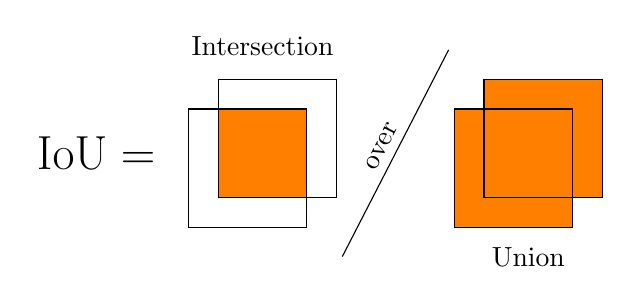
\begin{tikzpicture}[scale=0.75]
  \node[left] at (-0.4, 1.25) {\LARGE $\mathrm{IoU} = $};
  % Intersection illustration
  \begin{scope}
    \clip (0, 0) rectangle (2, 2);
    \fill[orange] (0.5, 0.5) rectangle (2.5, 2.5);
  \end{scope}
  \draw (0, 0) rectangle (2, 2);
  \draw (0.5, 0.5) rectangle (2.5, 2.5);
  \node[above, yshift=0.5em] at (1.25, 2.5) {Intersection};

  % Division sign
  \draw (2.6, -0.5) -- node[auto, sloped] {over} (4.4, 3);

  % Union illustration
  \begin{scope}[shift={(4.5, 0)}]
    \draw[fill=orange] (0, 0) rectangle (2, 2);
    \draw[fill=orange] (0.5, 0.5) rectangle (2.5, 2.5);
    \draw (0, 0) rectangle (2, 2);
    \node[below, yshift=-0.4em] at (1.25, 0) {Union};
  \end{scope}
\end{tikzpicture}

  \caption{%
    Visualization of single-class IoU metric.
  }%
  \label{fig:iou-metric}
\end{figure}

An alternative metric is the dice coefficient, often called the $F_1$ score as well.
The dice coefficient is defined by dividing twice the area of the intersection by the sum of the areas of the two masks:
%
\begin{equation*}
  \mathrm{F_1}
  =
  \frac{%
    2 \cdot |\mathrm{prediction} \cap \mathrm{truth}|
  }{%
    |\mathrm{prediction}| + |\mathrm{truth}|
  }
  =
  \frac{%
    \mathrm{2 \cdot TP}
  }{%
    2 \cdot \mathrm{TP} + \mathrm{FP} + \mathrm{FN}
  }.
\end{equation*}
%
Again we observe that this metric is bounded to the interval $[0, 1]$, with the same interpretation of the endpoints as with the IoU metric.
The visual representation of this metric is given in~\figref{fig:dice-coefficient}.

\begin{figure}[H]
  \centering
  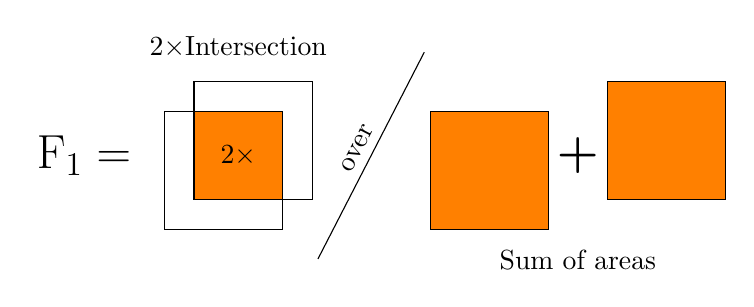
\begin{tikzpicture}[scale=0.75]
  \node[left] at (-0.4, 1.25) {\LARGE $\mathrm{F_1} = $};

  % Intersection illustration
  \begin{scope}
    \clip (0, 0) rectangle (2, 2);
    \fill[orange] (0.5, 0.5) rectangle (2.5, 2.5);
  \end{scope}
  \draw (0, 0) rectangle (2, 2);
  \draw (0.5, 0.5) rectangle (2.5, 2.5);
  \node[above, yshift=0.5em] at (1.25, 2.5) {$2 \times $Intersection};
  \node at (1.25, 1.25) {$2 \times$};

  % Division sign
  \draw (2.6, -0.5) -- node[auto, sloped] {over} (4.4, 3);

  % Union illustration
  \begin{scope}[shift={(4.5, 0)}]
    \draw[fill=orange] (0, 0) rectangle (2, 2);
    \begin{scope}[shift={(2.5, 0)}]
      \draw[fill=orange] (0.5, 0.5) rectangle (2.5, 2.5);
    \end{scope}
    \draw (0, 0) rectangle (2, 2);
    \node[below, yshift=-0.4em] at (2.5, 0) {Sum of areas};
    \node at (2.5, 1.25) {\LARGE \textbf{+}};
  \end{scope}
\end{tikzpicture}

  \caption{%
    Visualization of the single-class dice coefficient metric, also known as the $F_1$ score.
  }%
  \label{fig:dice-coefficient}
\end{figure}

You may have noticed that these two metrics are quite similar; they involve the same quantities, only weighted differently, and are bounded by to the same domain.
In fact, we can construct an exact relationship between these two metrics\footnote{The following relationship and the ensuing inequality bounds were noted by the \textit{Cross Validated Stack Exchange} user \enquote{Willem} here: \url{https://stats.stackexchange.com/a/276144}.}
%
\begin{equation*}
  \frac{%
    \mathrm{IoU}
  }{%
    \mathrm{F_1}
  }
  =
  \frac{1}{2}
  +
  \frac{%
    \mathrm{IoU}
  }{%
    2
  }.
\end{equation*}
%
The two metrics are therefore always positively correlated, as one metric increases or decreases, the other must necessarily follow suit.
A useful insight for how these two metrics actually differ is to observe how the IoU metric is bounded by the $\mathrm{F_1}$ metric:
%
\begin{equation*}
    \frac{%
      \mathrm{F_1}
    }{%
      2
    }
  \leq
    \mathrm{IoU}
  \leq
    \mathrm{F_1}
\end{equation*}
%
The IoU metric is \textit{always} less than or equal to the $\mathrm{F_1}$ metric, but never less than one half its value.
The fraction $\mathrm{IoU} / \mathrm{F_1}$ is equal to 1 whenever the prediction coincides with the ground truth and is equal to $1/2$ whenever there is no overlap at all.
By drawing an analogy to the $p = 1$ (absolute/Manhattan) norm and $p = 2$ (Euclidean) norm, the $\mathrm{IoU}$ metric is somewhat a reflection of the \textit{worst} performance, while the $\mathrm{F_1}$ metric is more a reflection of the \textit{average} performance of a given prediction.


  \topic{Binary cross-entropy and soft dice loss}
  So far all model experiments have been exclusively trained with the \textit{binary cross-entropy} loss function as given in equation~\eqref{eq:binary-cross-entropy}.
While this is the dominant loss function for binary classification tasks, it is still considered a suboptimal surrogate loss function for segmentation evaluation metrics such as the IoU metric.
Alternative loss functions were discussed in~\secref{sec:segmentation-metrics}, the so-called soft loss variants being of greatest interest.
Specifically, the \textit{soft Jaccard loss} given in equation~\eqref{eq:soft-jaccard-loss} and \textit{soft dice loss} given in equation~\eqref{eq:soft-dice-loss} having been theoretically and empirically shown to be efficient surrogate loss functions for the IoU metric.
Three models have been trained and evaluated, the only difference being which loss function that was used during training; binary cross-entropy, soft Jaccard loss, or soft dice loss.
The training procedures of these three models are visualized in \figref{fig:losses-training}.

\begin{figure}[H]
  \centering
  \includegraphics[width=0.66\linewidth]{metrics/lidar_dice_loss+lidar_jaccard_loss+without_rgb-validation-iou}
  \caption{%
    Three U-Net LiDAR models trained with different loss functions.
    Binary cross-entropy model shown in \textcolor{blue}{blue}, soft Jaccard in \textcolor{orange}{orange}, and soft dice shown in \textcolor{green}{green}.
  }%
  \label{fig:losses-training}
\end{figure}

The three models presented in~\figref{fig:losses-training} start out at approximately the same point after one epoch, but the binary cross-entropy model quickly outperforms the two other models when it comes to mean validation IoU.
The soft losses seem to be \emph{worse} surrogate losses for the IoU metric rather than better ones, completely contradicting our prior beliefs.

\begin{figure}[H]
  \centering
  \includegraphics[width=0.49\linewidth,trim={0 0.4cm 0 0.9cm},clip]{metric_correlation/without_rgb+lidar_jaccard_loss+iou}
  \textcolor{gray}{\vrule}
  \includegraphics[width=0.49\linewidth,trim={0 0.4cm 0 0.9cm},clip]{metric_correlation/without_rgb+lidar_dice_loss+iou}
  \caption{%
    Scatter plot showing the correlation between models using different losses during training.
    Both the left and right half of this figure compares model IoU against the binary cross-entropy IoU along the horizontal axis.
    Left figure half shows the soft Jaccard model on the vertical axis, while the right half shows the soft dice loss along the vertical axis.
    See caption of~\figref{fig:correlation-explanation} for detailed figure explanation.
  }
\end{figure}


\newpage
\subsection{State-of-the-Art}%
\label{sec:state-of-the-art}
We will give an overview of the current state of image segmentation.

\begin{itemize}
  \item Deep learning image segmentation overview given here~\cite{segmentation-overview} (\citeyear{segmentation-overview}).
  \item Recent semantic segmentation progress described here~\cite{segmentation-progress} (\citeyear{segmentation-progress}).
  \item Use of fully convolutional networks for semantic segmentation described here~\cite{segmentation-fcnn} (\citeyear{segmentation-fcnn}).
  \item SegNet architecture described here~\cite{segmentation-segnet} (\citeyear{segmentation-segnet}).
  \item U-Net architecture described here~\cite{segmentation-unet} (\citeyear{segmentation-unet}).
  \item Mask R-CNN architecture described here~\cite{segmentation-mask-r-cnn} (\citeyear{segmentation-mask-r-cnn}).
  \item SegCaps architecture described here~\cite{segmentation-segcaps} (\citeyear{segmentation-segcaps}).
  \item Panoptic feature pyramids described here~\cite{segmentation-panoptic-feature-pyramid} (\citeyear{segmentation-panoptic-feature-pyramid}).
\end{itemize}


  \section{Image Segmentation --- Central Concepts and Previous Work}
We will now present our numerical experiments, using the theory presented in~\secref{sec:segmentation} and data produced by the pipeline outlined in~\secref{sec:data}.
Specifically the U-Net model architecture is used for segmentation as previously described in~\secref{sec:unet}.
We start by describing the general experimental setup in~\secref{sec:experimental-setup}.
A comparative investigation into the suitability of the different raster data types (aerial photography and/or LiDAR DSMs) for predicting building outlines is presented in~\secref{sec:features}.
In~\secref{sec:technique-experiments} we try to determine if techniques intended to combat overfitting and aid training actually have their intended effect; specifically batch normalization, dropout, and data augmentation.
The different LiDAR normalization methods presented in \algref{alg:local-min-max-scaling} and \algref{alg:metric-normalization} are implemented and compared in~\secref{sec:normalization-experiment}.
Finally, \secref{sec:loss-experiment} presents the empirical efficiency of different surrogate loss functions.


\subsection{Problem Description}%
\label{sec:segmentation-description}
Image recognition seeks to answer three questions for any given image~\cite{image_recognition}:

\begin{enumerate}[nosep]
  \item \textbf{Identification:} Does the image contain any object of interest?
  \item \textbf{Localization:} Where in the image are the objects situated?
  \item \textbf{Classification:} To which categories do the objects belong to?
\end{enumerate}

We will concern ourselves with only one object category (class) at any time, that class being building footprints, and will simplify the following theory accordingly with this simplification in mind.
The localization and classification of objects in a given image can be performed at different granularity levels, as shown in~\figref{fig:segmentation-types}.

\begin{figure}[htb]
  \includegraphics[width=\linewidth,trim={0 4cm 0 3.4cm},clip]{segmentation-types}
  \caption{
    Different granularities for single-class building localization, using the Trondheim 2017 data set.
    Bounding box regression is shown on the left, semantic segmentation in the middle, and instance segmentation on the right.
  }%
  \label{fig:segmentation-types}
\end{figure}
\newpage

\textit{Bounding box regression} concerns itself with finding the smallest possible rectangles which envelopes the objects of interest.
The sides of the rectangles may either by oriented parallel to the axis directions, or rotated in order to attain the smallest possible envelope.
The bounding box will therefore necessarily contain pixels that are not part of the object itself whenever the object shape is not perfectly rectangular.

\textit{Semantic segmentation} rectifies this issue by classifying each pixel in the image independently, i.e. \textit{pixel-wise} classification, producing a so-called classification \textit{mask}.
\textit{Instance segmentation} distinguishes between pixels belonging to different objects of the same class, while \textit{semantic segmentation} does not make this distinction.
Since a bounding box can be directly derived from a semantic segmentation mask, and a semantic segmentation mask can be directly derived from instance segmentation mask; the problem complexity of these tasks are as follows:
%
\begin{equation*}
  \text{Bounding box regression}
  <
  \text{Semantic segmentation}
  <
  \text{Instance segmentation}
\end{equation*}
%
An image of width $W$ and height $H$ consisting of $C$ channels is represented by a $W \times H \times C$ tensor, $X \in \mathbb{R}^{W \times H \times C}$.
This is somewhat simplified, but we will give a more nuanced description in~\secref{sec:raster-data}.
Single-class semantic segmentation can therefore be formalized as constructing a binary predictor $\tilde{f}$ of the form:
%
\begin{equation*}
  \tilde{f}: \mathbb{R}^{W \times H \times C} \rightarrow \mathbb{B}^{W \times H}, \hspace{2em} \mathbb{B} \defeq \{0, 1\}.
\end{equation*}
%
Where $\mathbb{B}^{W \times H}$ denotes a boolean matrix, $1$ indicating that the pixel is part of the object class of interest, and $0$ indicates the opposite.
In practice, however, statistical models will often predict a pixel-wise class \textit{confidence} in the continuous domain $[0, 1]$,
%
\begin{equation*}
  \hat{f}: \mathbb{R}^{W \times H \times C} \rightarrow {[0, 1]}^{W \times H},
\end{equation*}
%
but a binary predictor can be easily constructed by choosing a suitable threshold, $T$, for which to distinguish positive predictions from negative ones
%
\begin{equation*}
  \tilde{f}(X) = \hat{f}(X) > T, \hspace{2em} X \in \mathbb{R}^{W \times H \times C}.
\end{equation*}
%
The choice of the threshold value $T$ will affect the resulting \textit{sensitivity} and \textit{specificity} metrics of the model predictions, metrics which will be explained in the upcoming~\secref{sec:segmentation-metrics}.


\subsection{Convolutional Neural Networks (CNNs)}%
\label{sec:cnn}
  \topic{Convolution}
  As the name implies, a central concept of convolutional neural networks is the so-called \textit{convolution operator}.
Let the \textit{kernel}, $w$, be a $H_k \times W_k$ real matrix, and denote the activation of the previous layer at position $(x, y)$ as $a_{x, y}$.
The \textit{convolution operator}, $\circledast$, is then defined as
%
\begin{align*}
  w \circledast a_{x, y} = \sum_{i} \sum_{j} w_{i, j} ~ a_{x - i, y - j},
  \hspace{3em}
    a_{x, y} \in \mathbb{R},~
    w \in \mathbb{R}^{H_k \times W_k},
\end{align*}
%
where $(i, j)$ spans the index set of the kernel.
The region around $a_{x,y}$ which is involved in the convolution is referred to as the \textit{receptive field}.
We can generate a \textit{filtered image} by moving this receptive field over the entire input image.
The step size used when moving the receptive field is referred to as the \textit{stride size} of the convolution.
This \textit{moving convolution} is illustrated in \figref{fig:convolution}.

\begin{figure}[htb]
  As the name implies, a central concept of convolutional neural networks is the so-called \textit{convolution operator}.
Let the \textit{kernel}, $w$, be a $H_k \times W_k$ real matrix, and denote the activation of the previous layer at position $(x, y)$ as $a_{x, y}$.
The \textit{convolution operator}, $\circledast$, is then defined as
%
\begin{align*}
  w \circledast a_{x, y} = \sum_{i} \sum_{j} w_{i, j} ~ a_{x - i, y - j},
  \hspace{3em}
    a_{x, y} \in \mathbb{R},~
    w \in \mathbb{R}^{H_k \times W_k},
\end{align*}
%
where $(i, j)$ spans the index set of the kernel.
The region around $a_{x,y}$ which is involved in the convolution is referred to as the \textit{receptive field}.
We can generate a \textit{filtered image} by moving this receptive field over the entire input image.
The step size used when moving the receptive field is referred to as the \textit{stride size} of the convolution.
This \textit{moving convolution} is illustrated in \figref{fig:convolution}.

\begin{figure}[htb]
  \input{tikz/convolution.tex}
  \caption{
    Visualization of a kernel convolution with a $3 \times 3$ kernel over an image of size $4 \times 4$ with additional zero-padding and stride size $1$.
    The \textit{receptive field} is shown in \textcolor{orange}{orange}, the respective kernel weights in \textcolor{blue}{blue}, and the resulting convolution output in \textcolor{green}{green}.
    Zero padding of the input image is shown in gray.
  }
  \label{fig:convolution}
\end{figure}

\todo{Finish this section. Some ideas are given below.}

How should we interpret the kernel?
The concept of a \textit{kernel} predates neural networks, and is used in image processing.
Kernel convolution can result in reduction of dimensionality.
The first cause for dimension reduction is that the kernel $(n \times m)$ kernel matrix, with $n, m \geq 1$ can't possibly applied to a $N \times M$ image exactly $N \cdot M$ times. The convolution can't be fit into the image that many times.
We will therefore lose information on the edges of the image after having applied the convolution.
The solution to this problem is to pad the image with zeros.
There are other ways to reduce the dimensionality with convolution.
A $4 \times 4$ kernel with stride $4 \times 4$ will reduce the resolution in both dimensions by four, for instance.

  \caption{
    Visualization of a kernel convolution with a $3 \times 3$ kernel over an image of size $4 \times 4$ with additional zero-padding and stride size $1$.
    The \textit{receptive field} is shown in \textcolor{orange}{orange}, the respective kernel weights in \textcolor{blue}{blue}, and the resulting convolution output in \textcolor{green}{green}.
    Zero padding of the input image is shown in gray.
  }
  \label{fig:convolution}
\end{figure}

\todo{Finish this section. Some ideas are given below.}

How should we interpret the kernel?
The concept of a \textit{kernel} predates neural networks, and is used in image processing.
Kernel convolution can result in reduction of dimensionality.
The first cause for dimension reduction is that the kernel $(n \times m)$ kernel matrix, with $n, m \geq 1$ can't possibly applied to a $N \times M$ image exactly $N \cdot M$ times. The convolution can't be fit into the image that many times.
We will therefore lose information on the edges of the image after having applied the convolution.
The solution to this problem is to pad the image with zeros.
There are other ways to reduce the dimensionality with convolution.
A $4 \times 4$ kernel with stride $4 \times 4$ will reduce the resolution in both dimensions by four, for instance.

  \topic{Activation functions}
  So far we have only explained how a convolutional neural network consists of a set of parametrized linear combinations.
Such networks, if left unaltered, are therefore restricted to only approximating linear functions.
The solution to this predicament is to introduce the concept of \textit{activation functions}, a nonlinear function applied to the output of the convolutional layers.
These activation functions were originally inspired by the neuroscientific understanding of biological neurons~\cite[p.~165]{goodfellow}, but have also been shown to be a theoretical prerequisite of the \textit{universal approximation} property of artificial neural networks~\cite{uat-sigmoid,uat-nonpolynomial}.
The \textit{logistic sigmoid} function, with its deep roots in probability theory, has been a popular choice for activation function in neural networks since the inception of the field~\cite{rosenblatt-perceptron-1958}, and is defined by
%
\begin{equation*}
  \sigma(x) = \frac{1}{1 + e^{-x}} = \frac{e^x}{e^x + 1}.
  \tag{Sigmoid activation function}
\end{equation*}
%
Observe that $\lim_{x \to -\infty} \sigma(x) = 0$ and $\lim_{x \to +\infty} \sigma(x) = 1$, and that the derivative is positive over the entire real number line. This makes it a bounded, differentiable, monotonic function, and is therefore suitable for mapping the weighted output of an artificial neuron in the domain $(-\infty, \infty)$ into the range $(0, 1)$.
This makes it especially suitable for the final layer in neural networks intended for predicting binary 0/1-responses.

Although the sigmoid activation function has a strong biological~\cite{rosenblatt-perceptron-1958} and theoretical~\cite{uat-sigmoid} underpinning, it suffers from the phenomenon of \textit{vanishing gradients} for network architectures consisting of three or more layers, which severely inhibits training.
As an alternative to the sigmoid activation function, the \textit{rectified linear unit} (ReLU) was introduced in a paper~\cite{relu-original-paper} by \citeauthor{relu-original-paper} in year \citeyear{relu-original-paper}.
It is defined as
%
\begin{equation*}
  \mathrm{ReLU}(x) = x^+ = \max(0, x).
  \tag{ReLU activation function}
\end{equation*}
%
The ReLU activation function has become the dominant activation function for use in neural networks in recent years~\cite[p.~438]{relu-popularity} as it has been empirically shown to adapt better to deeper neural networks~\cite{relu-better-than-sigmoid}.

  \topic{Pooling}
  %%%%%%%%%%%%%%%%%%% Local functions %%%%%%%%%%%%%%%%%%%
%% -- Draw marks
\newbox\dumbox% chktex 1
\newcommand{\mymark}[2]{%
  \setbox\dumbox=\hbox{#2}%
  \hbox to \wd\dumbox{\hss% chktex 1
    \tikz[overlay,remember picture,baseline=(#1.base)]{\node (#1) {\box\dumbox};}% chktex 36
    \hss}%
}

%%%%%%%%%%%%%%%%%%% Local functions %%%%%%%%%%%%%%%%%%%

\[
\underbracket[0.6pt][7pt]{
\left[\begin{array}{cccc}
  1 & 8 & \mymark{TL1}{5} & \mymark{TR1}{0} \\
  8 & 11 & \mymark{BL1}{5} & \mymark{BR1}{4} \\
  8 & 17 &               10 & 11               \\
  9 & 12 & 10 & 7 \\
\end{array}\right]
}_{\text{Activations}}
\hspace{0.5em}
\underbracket[0.6pt][7pt]{
\begin{array}{ccc}
    \mymark{TL2}{\phantom{1}} & \phantom{1} & \mymark{TR2}{\phantom{1}}\\
    \phantom{1}  & \mymark{mycenter}{\phantom{1}} &              \phantom{0} \\
    \mymark{BL2}{\phantom{1}} & \phantom{0} & \mymark{BR2}{\phantom{0}}
\end{array}
}_{\text{Pool operation}}
=
\underbracket[0.6pt][7pt]{
\left[\begin{array}{cccccc}
  11 & \mymark{C}{5} \\
  17 & 11 \\
\end{array}\right]
}_{\text{Pooled output}}
\]

\begin{tikzpicture}[overlay, remember picture,
    myedge1/.style={thin, opacity=.3, blue},
    myedge2/.style={thin, opacity=.3, green!40!black}]

  %% Draw boxes
  \draw[orange, fill=orange, fill opacity=.1]   (TL1.north west) rectangle (BR1.south east);
  \draw[blue, fill=blue, fill opacity=.1] (TL2.north west) rectangle (BR2.south east)
    node[midway, opacity=1, color=black] {\Large $\max$};
  \draw[green!60!black, fill=green, fill opacity=.1] (C.north west) rectangle (C.south east);

  %% Draw blue lines
  \draw[myedge1] (TL1.north west) -- (TL2.north west);
  \draw[myedge1] (BL1.south west) -- (BL2.south west);
  \draw[myedge1] (TR1.north east) -- (TR2.north east);
  \draw[myedge1] (BR1.south east) -- (BR2.south east);

  %% Draw green lines
  \draw[myedge2] (TL2.north west) -- (C.north west);
  \draw[myedge2] (BL2.south west) -- (C.south west);
  \draw[myedge2] (TR2.north east) -- (C.north east);
  \draw[myedge2] (BR2.south east) -- (C.south east);
\end{tikzpicture}

  \topic{Batch normalization}
  The reparametrization of earlier layers when training deep neural networks results in a distributional change in the feature layer forwarded to the next layers.
This forces all subsequent layers to adapt to the new \enquote{distributional circumstances}, which in turn impedes the convergence of the optimization.
This phenomenon, referred to as \textit{internal covariate shift}, was first identified in a paper~\cite{batch-normalization} by \citeauthor{batch-normalization}~(\citeyear{batch-normalization}) where they propose a method called \textit{batch normalization} in order to counter this phenomenon.
Suppose we have a layer activation $\vec{a}$ consisting of $d$ dimensions, i.e. $\vec{a} = (a^{(1)}, \ldots, a^{(d)})$.
First we standardize each feature dimension, $k$, independently

\begin{equation*}
  \widehat{a}^{(k)}
  =
  \frac{
    a^{(k)} - \E{a^{(k)}}
  }{
    \sqrt{\Var{a^{(k)}} + \epsilon}
  },
  \tag{Batch standardization}
\end{equation*}

where $\E{\cdot}$ and $\Var{\cdot}$ are respectively sample means and sample variances over the current mini-batch, and $\epsilon$ is added for numerical stability.
The result of this standardization is a feature map where all filters have mean $0$ and variance $1$ for every mini-batch.
The internal covariate shift has been practically eliminated as a result.

This type of normalization alone may not be optimal in all cases, though, and is best explained by constructing a somewhat contrived pathological example.
Assume a set of pooled layer activations $\vec{a}$ to be symmetrically distributed, and assume the subsequent convolution layer to preserve this symmetry.
After standardizing the output, 50\% of the values are expected to be negative, and all of these values will be truncated to $0$ if ReLU is the activation function of choice.
This informational loss may be suboptimal for the given network layer and must be accounted for.
That is to say, $\E{a} =  0$ and $\Var{a}$ may be an unsuitable domain for the given activation function.
For this reason, we introduce two additional trainable parameters for each feature dimension, $\gamma^{(k)}$ and $\beta^{(k)}$, and apply a second normalization step

\begin{equation*}
  y^{(k)} = \gamma^{(k)} \widehat{a}^{(k)} + \beta^{(k)}.
  \tag{Trainable normalization}
\end{equation*}

The intent is to learn the values for the shift, $\beta^{(k)}$, and scaler, $\gamma^{(k)}$, which restores the representative power of the given layer \textit{after} the batch standardization.

  \topic{Dropout}
  Dropout is a regularization technique for neural networks intended to prevent \enquote{complex co-adaption of feature detectors}~\cite{dropout-original-paper}.
In practice this is achieved by randomly omitting hidden nodes from the neural network during each training step; effectively forcing hidden nodes to become less interdependent.
An alternative interpretation of the dropout procedure is that it is a computationally efficient form of model averaging, each dropout permutation being a single model instance.
This technique has been empirically shown to significantly increase the test performance in several different settings.

Although originally intended for use in feedforward neural networks, dropout has been extensively applied in CNN architectures as well~\cite{dropout-cnn}.
Since there are no nodes to be omitted in convolutional architectures, the dropout procedure needs to be adapted in order to be applicable in a CNN setting.
One approach is to introduce a randomly located square mask (\textit{cutout}) to the input image~\cite{dropout-cutout}.
\textit{Stochastic depth dropout} randomly selects entire layers to be dropped, replacing them with identity functions instead~\cite{dropout-stochastic-depth}.
Dropout can also be integrated into max pooling layers, ignoring values at random during the search for the maximum value in the receptive field~\cite{max-pooling-dropout}.
This has become known as \textit{max-pooling dropout} and is illustrated in~\figref{fig:max-pooling-dropout}.

\begin{figure}[htb]
  %%%%%%%%%%%%%%%%%%% Local functions %%%%%%%%%%%%%%%%%%%
%% -- Draw marks
\newbox\dumbox% chktex 1
\newcommand{\mymark}[2]{%
  \setbox\dumbox=\hbox{#2}%
  \hbox to \wd\dumbox{\hss% chktex 1
    \tikz[overlay,remember picture,baseline=(#1.base)]{\node (#1) {\box\dumbox};}% chktex 36
    \hss}%
}
% Used to indicate dropout array indices
\newcommand{\dropout}[1]{{\setlength{\fboxsep}{0pt}\fcolorbox{black}{black}{#1}}}

%%%%%%%%%%%%%%%%%%% Local functions %%%%%%%%%%%%%%%%%%%

\begin{align*}
  \left[\begin{array}{cccc}
    1 & 8 & \mymark{oldTL1}{5} & \mymark{oldTR1}{0} \\
    8 & 11 & \mymark{oldBL1}{5} & \mymark{oldBR1}{4} \\
    8 & 17 &               10 & 11               \\
    9 & \mymark{old}{12} & 10 & 7 \\
  \end{array}\right]
  \hspace{0.5em}
  \begin{array}{ccc}
      \mymark{oldTL2}{\phantom{1}} & \phantom{1} & \mymark{oldTR2}{\phantom{1}}\\
      \phantom{1}  & \mymark{oldmycenter}{\phantom{1}} &              \phantom{0} \\
      \mymark{oldBL2}{\phantom{1}} & \phantom{0} & \mymark{oldBR2}{\phantom{0}}
  \end{array}
  =
  \left[\begin{array}{cccccc}
    11 & \mymark{oldC}{5} \\
    17 & 11 \\
  \end{array}\right]
  \\[2.25em]
  \left[\begin{array}{cccc}
    1 & \mymark{new}{8} & \mymark{TL1}{\dropout{5}} & \mymark{TR1}{0} \\
    \dropout{8} & 11 & \mymark{BL1}{\dropout{5}} & \mymark{BR1}{4} \\
    8 & \dropout{1} &               10 & 11               \\
    \dropout{9} & 12 & 10 & 7 \\
  \end{array}\right]
  \hspace{0.5em}
  \begin{array}{ccc}
      \mymark{TL2}{\phantom{1}} & \phantom{1} & \mymark{TR2}{\phantom{1}}\\
      \phantom{1}  & \mymark{mycenter}{\phantom{1}} &              \phantom{0} \\
      \mymark{BL2}{\phantom{1}} & \phantom{0} & \mymark{BR2}{\phantom{0}}
  \end{array}
  =
  \left[\begin{array}{cccccc}
    11 & \mymark{C}{4} \\
    12 & 11 \\
  \end{array}\right]
\end{align*}

\begin{tikzpicture}[overlay, remember picture,
    myedge1/.style={thin, opacity=.3, blue},
    myedge2/.style={thin, opacity=.3, green!40!black}]

  %% Draw boxes
  \draw[orange, fill=orange, fill opacity=.1]   (TL1.north west) rectangle (BR1.south east);
  \draw[orange, fill=orange, fill opacity=.1]   (oldTL1.north west) rectangle (oldBR1.south east);

  \draw[blue, fill=blue, fill opacity=.1] (TL2.north west) rectangle (BR2.south east)
    node[midway, opacity=1, color=black] {\Large $\max$};
  \draw[blue, fill=blue, fill opacity=.1] (oldTL2.north west) rectangle (oldBR2.south east)
    node[midway, opacity=1, color=black] {\Large $\max$};

  \draw[green!60!black, fill=green, fill opacity=.1] (C.north west) rectangle (C.south east);
  \draw[green!60!black, fill=green, fill opacity=.1] (oldC.north west) rectangle (oldC.south east);

  %% Draw blue lines
  \draw[myedge1] (TL1.north west) -- (TL2.north west);
  \draw[myedge1] (BL1.south west) -- (BL2.south west);
  \draw[myedge1] (TR1.north east) -- (TR2.north east);
  \draw[myedge1] (BR1.south east) -- (BR2.south east);
  \draw[myedge1] (oldTL1.north west) -- (oldTL2.north west);
  \draw[myedge1] (oldBL1.south west) -- (oldBL2.south west);
  \draw[myedge1] (oldTR1.north east) -- (oldTR2.north east);
  \draw[myedge1] (oldBR1.south east) -- (oldBR2.south east);

  %% Draw green lines
  \draw[myedge2] (TL2.north west) -- (C.north west);
  \draw[myedge2] (BL2.south west) -- (C.south west);
  \draw[myedge2] (TR2.north east) -- (C.north east);
  \draw[myedge2] (BR2.south east) -- (C.south east);
  \draw[myedge2] (oldTL2.north west) -- (oldC.north west);
  \draw[myedge2] (oldBL2.south west) -- (oldC.south west);
  \draw[myedge2] (oldTR2.north east) -- (oldC.north east);
  \draw[myedge2] (oldBR2.south east) -- (oldC.south east);

  % Draw arrow from old to new activation matrix
  \draw[->, line width=0.5mm, shorten >= 2mm] (old) ++ (-0.1mm, -4mm) -- node[auto, yshift=1mm] {Dropout} (new.north);
\end{tikzpicture}

  \caption{%
    An example application of \textit{max-pooling dropout} using a receptive field and stride of size $2 \times 2$.
    A dropout probability of $p = 0.25$ has been used.
    Dropped values are shown as black boxes.
  }%
  \label{fig:max-pooling-dropout}
\end{figure}


\subsection{Metrics and Losses}%
\label{sec:segmentation-metrics}
We will now present our numerical experiments, using the theory presented in~\secref{sec:segmentation} and data produced by the pipeline outlined in~\secref{sec:data}.
Specifically the U-Net model architecture is used for segmentation as previously described in~\secref{sec:unet}.
We start by describing the general experimental setup in~\secref{sec:experimental-setup}.
A comparative investigation into the suitability of the different raster data types (aerial photography and/or LiDAR DSMs) for predicting building outlines is presented in~\secref{sec:features}.
In~\secref{sec:technique-experiments} we try to determine if techniques intended to combat overfitting and aid training actually have their intended effect; specifically batch normalization, dropout, and data augmentation.
The different LiDAR normalization methods presented in \algref{alg:local-min-max-scaling} and \algref{alg:metric-normalization} are implemented and compared in~\secref{sec:normalization-experiment}.
Finally, \secref{sec:loss-experiment} presents the empirical efficiency of different surrogate loss functions.

  \topic{Accuracy, sensitivity, and specificity}
  In order to describe segmentation metrics, it is useful to define the following quantities:

\begin{center}
  \fbox{
    \parbox{0.9\linewidth}{
      \begin{description}[font=\sffamily\bfseries, leftmargin=1cm]
        \item[Condition Positive (P)]
          Number of object class pixels in ground truth mask.
        \item[Condition Negative (N)]
          Number of non-object class pixels in ground truth mask.
        \item[True Positive (TP)]
          Number of pixels correctly predicted as being part of object class (correctly identified).
        \item[True Negative (TN)]
          Number of pixels correctly predicted as \textit{not} being part of object class (correctly rejected).
        \item[False Positive (FP)]
          Number of pixel incorrectly predicted as being part of object class (incorrectly identified).
        \item[False Negative (FN)]
          Number of pixel incorrectly predicted as \textit{not} being part of object class (incorrectly rejected).
      \end{description}
    }
  }
\end{center}

False positives (FP) are often knows as \textit{type I errors} in statistics, and false negatives (FN) as \textit{Type II errors}.
The greater the values of TP and TN, the better, and the smaller the values of FP and FN, the better.
A visual representation of these classifications is given in~\figref{fig:confusions}.

\begin{figure}[htb]
  \includegraphics[width=\linewidth]{confusions}
  \caption{
    Binary segmentation problem of size $256 \times 256$.
    The ground truth, a rectangle of size $120 \times 80$ is shown on the left.
    The \enquote{predicted} mask, shown in the middle, is of the same size, but offset by $(-30, -30)$.
    The right figure shows the visual equivalent of a confusion matrix.
    True positives are shown in \textcolor{tp}{dark blue}, true negatives in \textcolor{gray}{light gray}, false positives in \textcolor{fp}{green}, and false negatives in \textcolor{fn}{red}.
  }%
  \label{fig:confusions}
\end{figure}

The simplest metric for semantic segmentation is the \textit{pixel accuracy} metric.
This metric simply reports the percentage of pixels that were correctly classified.
More formally, it can be defined as:

\begin{equation*}
    \textbf{accuracy} = \frac{TP + TN}{TP + TN + FP + FN} = \frac{TP + TN}{P + N}
\end{equation*}

The problem with pixel-wise accuracy metrics is that it does not account for class imbalances.
Consider a problem where 95\% of all pixels are considered to be of class $0$, and the remaining 5\% of class $1$.
If we construct a model which predicts $0$ regardless of the feature inputs provided to the model, the model will achieve a 95\% accuracy score.
This makes pixel-wise accuracy scores difficult to interpret when you do not know the class balance of the respective dataset and the accuracy grouped by class.
This is why it is often replaced by other metrics which takes imbalances into account.
A pair of such metrics is \textit{sensitivity} and \textit{specificity}, formally defined as:

\begin{align*}
    \textbf{sensitivity}
    &=
    \frac{\text{number of true positives}}{\text{number of true positives + number of false negatives}}
    =
    \frac{TP}{TP + FN}
    =
    \frac{TP}{P}
    \\
    \textbf{specificity}
    &=
    \frac{\text{number of true negatives}}{\text{number of true negatives + number of false positives}}
    =
    \frac{TN}{TN + FP}
    =
    \frac{TN}{N}
\end{align*}

The \textit{sensitivity} is therefore a measure of how good the given model prediction was able to identify positives as a relative, fractional value.
Likewise, the \textit{specificity} is a measure of how good the given model prediction was able to identify negatives as a relative, fractional value.


  \topic{Intersection over union and dice coefficient}
  Although the sensitivity and specificity metrics address the issue of class imbalances, they are still \textit{two} distinct metrics that need to be simultaneously inspected in order to get a full performance picture of a given prediction.
We now pose the following problem: \enquote{is it possible to construct a \textit{single} scalar metric which incorporates the idea of sensitivity and specificity?}.
The \textit{intersection over union} (IoU) and \textit{dice coefficient} ($F_1$) are two attempts at solving this problem.

The IoU metric is defined as the area of the intersection between the predicted segmentation mask and the ground truth mask divided by the union of these two masks, or more formally
%
\begin{equation*}
  \mathrm{IoU}
  =
  \frac{%
    |\mathrm{prediction} \cap \mathrm{truth}|
  }{%
    |\mathrm{prediction} \cup \mathrm{truth}|
  }
  =
  \frac{%
    \mathrm{TP}
  }{%
    \mathrm{TP} + \mathrm{FP} + \mathrm{FN}
  }.
\end{equation*}
%
In the case of multiple classes IoU is calculated for each class independently and the result is averaged, known as \textit{mean intersection over union} (MIoU).
MIoU is the most commonly used segmentation metric in research and competitions due to its simplicity and representativeness~\cite{segmentation-overview}.
Notice how the IoU metric is bounded between 0 and 1; $\mathrm{IoU} = 0$ representing a complete \enquote{predictive miss} and $\mathrm{IoU} = 1$ representing a prediction in perfect accordance with the ground truth.
A visualization of this metric is given in \figref{fig:iou-metric} below.

\begin{figure}[H]
  \centering
  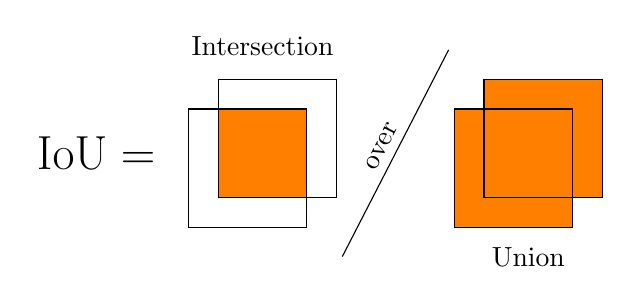
\begin{tikzpicture}[scale=0.75]
  \node[left] at (-0.4, 1.25) {\LARGE $\mathrm{IoU} = $};
  % Intersection illustration
  \begin{scope}
    \clip (0, 0) rectangle (2, 2);
    \fill[orange] (0.5, 0.5) rectangle (2.5, 2.5);
  \end{scope}
  \draw (0, 0) rectangle (2, 2);
  \draw (0.5, 0.5) rectangle (2.5, 2.5);
  \node[above, yshift=0.5em] at (1.25, 2.5) {Intersection};

  % Division sign
  \draw (2.6, -0.5) -- node[auto, sloped] {over} (4.4, 3);

  % Union illustration
  \begin{scope}[shift={(4.5, 0)}]
    \draw[fill=orange] (0, 0) rectangle (2, 2);
    \draw[fill=orange] (0.5, 0.5) rectangle (2.5, 2.5);
    \draw (0, 0) rectangle (2, 2);
    \node[below, yshift=-0.4em] at (1.25, 0) {Union};
  \end{scope}
\end{tikzpicture}

  \caption{%
    Visualization of single-class IoU metric.
  }%
  \label{fig:iou-metric}
\end{figure}

An alternative metric is the dice coefficient, often called the $F_1$ score as well.
The dice coefficient is defined by dividing twice the area of the intersection by the sum of the areas of the two masks:
%
\begin{equation*}
  \mathrm{F_1}
  =
  \frac{%
    2 \cdot |\mathrm{prediction} \cap \mathrm{truth}|
  }{%
    |\mathrm{prediction}| + |\mathrm{truth}|
  }
  =
  \frac{%
    \mathrm{2 \cdot TP}
  }{%
    2 \cdot \mathrm{TP} + \mathrm{FP} + \mathrm{FN}
  }.
\end{equation*}
%
Again we observe that this metric is bounded to the interval $[0, 1]$, with the same interpretation of the endpoints as with the IoU metric.
The visual representation of this metric is given in~\figref{fig:dice-coefficient}.

\begin{figure}[H]
  \centering
  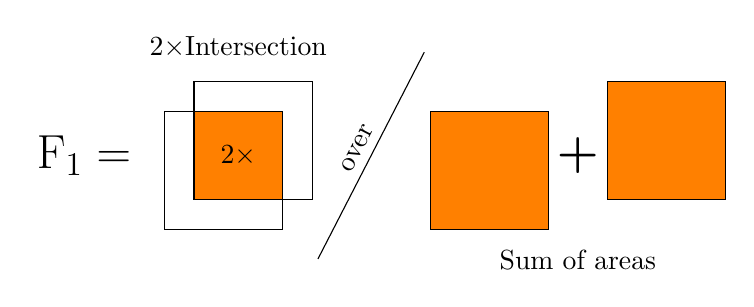
\begin{tikzpicture}[scale=0.75]
  \node[left] at (-0.4, 1.25) {\LARGE $\mathrm{F_1} = $};

  % Intersection illustration
  \begin{scope}
    \clip (0, 0) rectangle (2, 2);
    \fill[orange] (0.5, 0.5) rectangle (2.5, 2.5);
  \end{scope}
  \draw (0, 0) rectangle (2, 2);
  \draw (0.5, 0.5) rectangle (2.5, 2.5);
  \node[above, yshift=0.5em] at (1.25, 2.5) {$2 \times $Intersection};
  \node at (1.25, 1.25) {$2 \times$};

  % Division sign
  \draw (2.6, -0.5) -- node[auto, sloped] {over} (4.4, 3);

  % Union illustration
  \begin{scope}[shift={(4.5, 0)}]
    \draw[fill=orange] (0, 0) rectangle (2, 2);
    \begin{scope}[shift={(2.5, 0)}]
      \draw[fill=orange] (0.5, 0.5) rectangle (2.5, 2.5);
    \end{scope}
    \draw (0, 0) rectangle (2, 2);
    \node[below, yshift=-0.4em] at (2.5, 0) {Sum of areas};
    \node at (2.5, 1.25) {\LARGE \textbf{+}};
  \end{scope}
\end{tikzpicture}

  \caption{%
    Visualization of the single-class dice coefficient metric, also known as the $F_1$ score.
  }%
  \label{fig:dice-coefficient}
\end{figure}

You may have noticed that these two metrics are quite similar; they involve the same quantities, only weighted differently, and are bounded by to the same domain.
In fact, we can construct an exact relationship between these two metrics\footnote{The following relationship and the ensuing inequality bounds were noted by the \textit{Cross Validated Stack Exchange} user \enquote{Willem} here: \url{https://stats.stackexchange.com/a/276144}.}
%
\begin{equation*}
  \frac{%
    \mathrm{IoU}
  }{%
    \mathrm{F_1}
  }
  =
  \frac{1}{2}
  +
  \frac{%
    \mathrm{IoU}
  }{%
    2
  }.
\end{equation*}
%
The two metrics are therefore always positively correlated, as one metric increases or decreases, the other must necessarily follow suit.
A useful insight for how these two metrics actually differ is to observe how the IoU metric is bounded by the $\mathrm{F_1}$ metric:
%
\begin{equation*}
    \frac{%
      \mathrm{F_1}
    }{%
      2
    }
  \leq
    \mathrm{IoU}
  \leq
    \mathrm{F_1}
\end{equation*}
%
The IoU metric is \textit{always} less than or equal to the $\mathrm{F_1}$ metric, but never less than one half its value.
The fraction $\mathrm{IoU} / \mathrm{F_1}$ is equal to 1 whenever the prediction coincides with the ground truth and is equal to $1/2$ whenever there is no overlap at all.
By drawing an analogy to the $p = 1$ (absolute/Manhattan) norm and $p = 2$ (Euclidean) norm, the $\mathrm{IoU}$ metric is somewhat a reflection of the \textit{worst} performance, while the $\mathrm{F_1}$ metric is more a reflection of the \textit{average} performance of a given prediction.


  \topic{Binary cross-entropy and soft dice loss}
  So far all model experiments have been exclusively trained with the \textit{binary cross-entropy} loss function as given in equation~\eqref{eq:binary-cross-entropy}.
While this is the dominant loss function for binary classification tasks, it is still considered a suboptimal surrogate loss function for segmentation evaluation metrics such as the IoU metric.
Alternative loss functions were discussed in~\secref{sec:segmentation-metrics}, the so-called soft loss variants being of greatest interest.
Specifically, the \textit{soft Jaccard loss} given in equation~\eqref{eq:soft-jaccard-loss} and \textit{soft dice loss} given in equation~\eqref{eq:soft-dice-loss} having been theoretically and empirically shown to be efficient surrogate loss functions for the IoU metric.
Three models have been trained and evaluated, the only difference being which loss function that was used during training; binary cross-entropy, soft Jaccard loss, or soft dice loss.
The training procedures of these three models are visualized in \figref{fig:losses-training}.

\begin{figure}[H]
  \centering
  \includegraphics[width=0.66\linewidth]{metrics/lidar_dice_loss+lidar_jaccard_loss+without_rgb-validation-iou}
  \caption{%
    Three U-Net LiDAR models trained with different loss functions.
    Binary cross-entropy model shown in \textcolor{blue}{blue}, soft Jaccard in \textcolor{orange}{orange}, and soft dice shown in \textcolor{green}{green}.
  }%
  \label{fig:losses-training}
\end{figure}

The three models presented in~\figref{fig:losses-training} start out at approximately the same point after one epoch, but the binary cross-entropy model quickly outperforms the two other models when it comes to mean validation IoU.
The soft losses seem to be \emph{worse} surrogate losses for the IoU metric rather than better ones, completely contradicting our prior beliefs.

\begin{figure}[H]
  \centering
  \includegraphics[width=0.49\linewidth,trim={0 0.4cm 0 0.9cm},clip]{metric_correlation/without_rgb+lidar_jaccard_loss+iou}
  \textcolor{gray}{\vrule}
  \includegraphics[width=0.49\linewidth,trim={0 0.4cm 0 0.9cm},clip]{metric_correlation/without_rgb+lidar_dice_loss+iou}
  \caption{%
    Scatter plot showing the correlation between models using different losses during training.
    Both the left and right half of this figure compares model IoU against the binary cross-entropy IoU along the horizontal axis.
    Left figure half shows the soft Jaccard model on the vertical axis, while the right half shows the soft dice loss along the vertical axis.
    See caption of~\figref{fig:correlation-explanation} for detailed figure explanation.
  }
\end{figure}


\newpage
\subsection{State-of-the-Art}%
\label{sec:state-of-the-art}
We will give an overview of the current state of image segmentation.

\begin{itemize}
  \item Deep learning image segmentation overview given here~\cite{segmentation-overview} (\citeyear{segmentation-overview}).
  \item Recent semantic segmentation progress described here~\cite{segmentation-progress} (\citeyear{segmentation-progress}).
  \item Use of fully convolutional networks for semantic segmentation described here~\cite{segmentation-fcnn} (\citeyear{segmentation-fcnn}).
  \item SegNet architecture described here~\cite{segmentation-segnet} (\citeyear{segmentation-segnet}).
  \item U-Net architecture described here~\cite{segmentation-unet} (\citeyear{segmentation-unet}).
  \item Mask R-CNN architecture described here~\cite{segmentation-mask-r-cnn} (\citeyear{segmentation-mask-r-cnn}).
  \item SegCaps architecture described here~\cite{segmentation-segcaps} (\citeyear{segmentation-segcaps}).
  \item Panoptic feature pyramids described here~\cite{segmentation-panoptic-feature-pyramid} (\citeyear{segmentation-panoptic-feature-pyramid}).
\end{itemize}


  \section{Image Segmentation --- Central Concepts and Previous Work}
We will now present our numerical experiments, using the theory presented in~\secref{sec:segmentation} and data produced by the pipeline outlined in~\secref{sec:data}.
Specifically the U-Net model architecture is used for segmentation as previously described in~\secref{sec:unet}.
We start by describing the general experimental setup in~\secref{sec:experimental-setup}.
A comparative investigation into the suitability of the different raster data types (aerial photography and/or LiDAR DSMs) for predicting building outlines is presented in~\secref{sec:features}.
In~\secref{sec:technique-experiments} we try to determine if techniques intended to combat overfitting and aid training actually have their intended effect; specifically batch normalization, dropout, and data augmentation.
The different LiDAR normalization methods presented in \algref{alg:local-min-max-scaling} and \algref{alg:metric-normalization} are implemented and compared in~\secref{sec:normalization-experiment}.
Finally, \secref{sec:loss-experiment} presents the empirical efficiency of different surrogate loss functions.


\subsection{Problem Description}%
\label{sec:segmentation-description}
Image recognition seeks to answer three questions for any given image~\cite{image_recognition}:

\begin{enumerate}[nosep]
  \item \textbf{Identification:} Does the image contain any object of interest?
  \item \textbf{Localization:} Where in the image are the objects situated?
  \item \textbf{Classification:} To which categories do the objects belong to?
\end{enumerate}

We will concern ourselves with only one object category (class) at any time, that class being building footprints, and will simplify the following theory accordingly with this simplification in mind.
The localization and classification of objects in a given image can be performed at different granularity levels, as shown in~\figref{fig:segmentation-types}.

\begin{figure}[htb]
  \includegraphics[width=\linewidth,trim={0 4cm 0 3.4cm},clip]{segmentation-types}
  \caption{
    Different granularities for single-class building localization, using the Trondheim 2017 data set.
    Bounding box regression is shown on the left, semantic segmentation in the middle, and instance segmentation on the right.
  }%
  \label{fig:segmentation-types}
\end{figure}
\newpage

\textit{Bounding box regression} concerns itself with finding the smallest possible rectangles which envelopes the objects of interest.
The sides of the rectangles may either by oriented parallel to the axis directions, or rotated in order to attain the smallest possible envelope.
The bounding box will therefore necessarily contain pixels that are not part of the object itself whenever the object shape is not perfectly rectangular.

\textit{Semantic segmentation} rectifies this issue by classifying each pixel in the image independently, i.e. \textit{pixel-wise} classification, producing a so-called classification \textit{mask}.
\textit{Instance segmentation} distinguishes between pixels belonging to different objects of the same class, while \textit{semantic segmentation} does not make this distinction.
Since a bounding box can be directly derived from a semantic segmentation mask, and a semantic segmentation mask can be directly derived from instance segmentation mask; the problem complexity of these tasks are as follows:
%
\begin{equation*}
  \text{Bounding box regression}
  <
  \text{Semantic segmentation}
  <
  \text{Instance segmentation}
\end{equation*}
%
An image of width $W$ and height $H$ consisting of $C$ channels is represented by a $W \times H \times C$ tensor, $X \in \mathbb{R}^{W \times H \times C}$.
This is somewhat simplified, but we will give a more nuanced description in~\secref{sec:raster-data}.
Single-class semantic segmentation can therefore be formalized as constructing a binary predictor $\tilde{f}$ of the form:
%
\begin{equation*}
  \tilde{f}: \mathbb{R}^{W \times H \times C} \rightarrow \mathbb{B}^{W \times H}, \hspace{2em} \mathbb{B} \defeq \{0, 1\}.
\end{equation*}
%
Where $\mathbb{B}^{W \times H}$ denotes a boolean matrix, $1$ indicating that the pixel is part of the object class of interest, and $0$ indicates the opposite.
In practice, however, statistical models will often predict a pixel-wise class \textit{confidence} in the continuous domain $[0, 1]$,
%
\begin{equation*}
  \hat{f}: \mathbb{R}^{W \times H \times C} \rightarrow {[0, 1]}^{W \times H},
\end{equation*}
%
but a binary predictor can be easily constructed by choosing a suitable threshold, $T$, for which to distinguish positive predictions from negative ones
%
\begin{equation*}
  \tilde{f}(X) = \hat{f}(X) > T, \hspace{2em} X \in \mathbb{R}^{W \times H \times C}.
\end{equation*}
%
The choice of the threshold value $T$ will affect the resulting \textit{sensitivity} and \textit{specificity} metrics of the model predictions, metrics which will be explained in the upcoming~\secref{sec:segmentation-metrics}.


\subsection{Convolutional Neural Networks (CNNs)}%
\label{sec:cnn}
  \topic{Convolution}
  As the name implies, a central concept of convolutional neural networks is the so-called \textit{convolution operator}.
Let the \textit{kernel}, $w$, be a $H_k \times W_k$ real matrix, and denote the activation of the previous layer at position $(x, y)$ as $a_{x, y}$.
The \textit{convolution operator}, $\circledast$, is then defined as
%
\begin{align*}
  w \circledast a_{x, y} = \sum_{i} \sum_{j} w_{i, j} ~ a_{x - i, y - j},
  \hspace{3em}
    a_{x, y} \in \mathbb{R},~
    w \in \mathbb{R}^{H_k \times W_k},
\end{align*}
%
where $(i, j)$ spans the index set of the kernel.
The region around $a_{x,y}$ which is involved in the convolution is referred to as the \textit{receptive field}.
We can generate a \textit{filtered image} by moving this receptive field over the entire input image.
The step size used when moving the receptive field is referred to as the \textit{stride size} of the convolution.
This \textit{moving convolution} is illustrated in \figref{fig:convolution}.

\begin{figure}[htb]
  As the name implies, a central concept of convolutional neural networks is the so-called \textit{convolution operator}.
Let the \textit{kernel}, $w$, be a $H_k \times W_k$ real matrix, and denote the activation of the previous layer at position $(x, y)$ as $a_{x, y}$.
The \textit{convolution operator}, $\circledast$, is then defined as
%
\begin{align*}
  w \circledast a_{x, y} = \sum_{i} \sum_{j} w_{i, j} ~ a_{x - i, y - j},
  \hspace{3em}
    a_{x, y} \in \mathbb{R},~
    w \in \mathbb{R}^{H_k \times W_k},
\end{align*}
%
where $(i, j)$ spans the index set of the kernel.
The region around $a_{x,y}$ which is involved in the convolution is referred to as the \textit{receptive field}.
We can generate a \textit{filtered image} by moving this receptive field over the entire input image.
The step size used when moving the receptive field is referred to as the \textit{stride size} of the convolution.
This \textit{moving convolution} is illustrated in \figref{fig:convolution}.

\begin{figure}[htb]
  \input{tikz/convolution.tex}
  \caption{
    Visualization of a kernel convolution with a $3 \times 3$ kernel over an image of size $4 \times 4$ with additional zero-padding and stride size $1$.
    The \textit{receptive field} is shown in \textcolor{orange}{orange}, the respective kernel weights in \textcolor{blue}{blue}, and the resulting convolution output in \textcolor{green}{green}.
    Zero padding of the input image is shown in gray.
  }
  \label{fig:convolution}
\end{figure}

\todo{Finish this section. Some ideas are given below.}

How should we interpret the kernel?
The concept of a \textit{kernel} predates neural networks, and is used in image processing.
Kernel convolution can result in reduction of dimensionality.
The first cause for dimension reduction is that the kernel $(n \times m)$ kernel matrix, with $n, m \geq 1$ can't possibly applied to a $N \times M$ image exactly $N \cdot M$ times. The convolution can't be fit into the image that many times.
We will therefore lose information on the edges of the image after having applied the convolution.
The solution to this problem is to pad the image with zeros.
There are other ways to reduce the dimensionality with convolution.
A $4 \times 4$ kernel with stride $4 \times 4$ will reduce the resolution in both dimensions by four, for instance.

  \caption{
    Visualization of a kernel convolution with a $3 \times 3$ kernel over an image of size $4 \times 4$ with additional zero-padding and stride size $1$.
    The \textit{receptive field} is shown in \textcolor{orange}{orange}, the respective kernel weights in \textcolor{blue}{blue}, and the resulting convolution output in \textcolor{green}{green}.
    Zero padding of the input image is shown in gray.
  }
  \label{fig:convolution}
\end{figure}

\todo{Finish this section. Some ideas are given below.}

How should we interpret the kernel?
The concept of a \textit{kernel} predates neural networks, and is used in image processing.
Kernel convolution can result in reduction of dimensionality.
The first cause for dimension reduction is that the kernel $(n \times m)$ kernel matrix, with $n, m \geq 1$ can't possibly applied to a $N \times M$ image exactly $N \cdot M$ times. The convolution can't be fit into the image that many times.
We will therefore lose information on the edges of the image after having applied the convolution.
The solution to this problem is to pad the image with zeros.
There are other ways to reduce the dimensionality with convolution.
A $4 \times 4$ kernel with stride $4 \times 4$ will reduce the resolution in both dimensions by four, for instance.

  \topic{Activation functions}
  So far we have only explained how a convolutional neural network consists of a set of parametrized linear combinations.
Such networks, if left unaltered, are therefore restricted to only approximating linear functions.
The solution to this predicament is to introduce the concept of \textit{activation functions}, a nonlinear function applied to the output of the convolutional layers.
These activation functions were originally inspired by the neuroscientific understanding of biological neurons~\cite[p.~165]{goodfellow}, but have also been shown to be a theoretical prerequisite of the \textit{universal approximation} property of artificial neural networks~\cite{uat-sigmoid,uat-nonpolynomial}.
The \textit{logistic sigmoid} function, with its deep roots in probability theory, has been a popular choice for activation function in neural networks since the inception of the field~\cite{rosenblatt-perceptron-1958}, and is defined by
%
\begin{equation*}
  \sigma(x) = \frac{1}{1 + e^{-x}} = \frac{e^x}{e^x + 1}.
  \tag{Sigmoid activation function}
\end{equation*}
%
Observe that $\lim_{x \to -\infty} \sigma(x) = 0$ and $\lim_{x \to +\infty} \sigma(x) = 1$, and that the derivative is positive over the entire real number line. This makes it a bounded, differentiable, monotonic function, and is therefore suitable for mapping the weighted output of an artificial neuron in the domain $(-\infty, \infty)$ into the range $(0, 1)$.
This makes it especially suitable for the final layer in neural networks intended for predicting binary 0/1-responses.

Although the sigmoid activation function has a strong biological~\cite{rosenblatt-perceptron-1958} and theoretical~\cite{uat-sigmoid} underpinning, it suffers from the phenomenon of \textit{vanishing gradients} for network architectures consisting of three or more layers, which severely inhibits training.
As an alternative to the sigmoid activation function, the \textit{rectified linear unit} (ReLU) was introduced in a paper~\cite{relu-original-paper} by \citeauthor{relu-original-paper} in year \citeyear{relu-original-paper}.
It is defined as
%
\begin{equation*}
  \mathrm{ReLU}(x) = x^+ = \max(0, x).
  \tag{ReLU activation function}
\end{equation*}
%
The ReLU activation function has become the dominant activation function for use in neural networks in recent years~\cite[p.~438]{relu-popularity} as it has been empirically shown to adapt better to deeper neural networks~\cite{relu-better-than-sigmoid}.

  \topic{Pooling}
  %%%%%%%%%%%%%%%%%%% Local functions %%%%%%%%%%%%%%%%%%%
%% -- Draw marks
\newbox\dumbox% chktex 1
\newcommand{\mymark}[2]{%
  \setbox\dumbox=\hbox{#2}%
  \hbox to \wd\dumbox{\hss% chktex 1
    \tikz[overlay,remember picture,baseline=(#1.base)]{\node (#1) {\box\dumbox};}% chktex 36
    \hss}%
}

%%%%%%%%%%%%%%%%%%% Local functions %%%%%%%%%%%%%%%%%%%

\[
\underbracket[0.6pt][7pt]{
\left[\begin{array}{cccc}
  1 & 8 & \mymark{TL1}{5} & \mymark{TR1}{0} \\
  8 & 11 & \mymark{BL1}{5} & \mymark{BR1}{4} \\
  8 & 17 &               10 & 11               \\
  9 & 12 & 10 & 7 \\
\end{array}\right]
}_{\text{Activations}}
\hspace{0.5em}
\underbracket[0.6pt][7pt]{
\begin{array}{ccc}
    \mymark{TL2}{\phantom{1}} & \phantom{1} & \mymark{TR2}{\phantom{1}}\\
    \phantom{1}  & \mymark{mycenter}{\phantom{1}} &              \phantom{0} \\
    \mymark{BL2}{\phantom{1}} & \phantom{0} & \mymark{BR2}{\phantom{0}}
\end{array}
}_{\text{Pool operation}}
=
\underbracket[0.6pt][7pt]{
\left[\begin{array}{cccccc}
  11 & \mymark{C}{5} \\
  17 & 11 \\
\end{array}\right]
}_{\text{Pooled output}}
\]

\begin{tikzpicture}[overlay, remember picture,
    myedge1/.style={thin, opacity=.3, blue},
    myedge2/.style={thin, opacity=.3, green!40!black}]

  %% Draw boxes
  \draw[orange, fill=orange, fill opacity=.1]   (TL1.north west) rectangle (BR1.south east);
  \draw[blue, fill=blue, fill opacity=.1] (TL2.north west) rectangle (BR2.south east)
    node[midway, opacity=1, color=black] {\Large $\max$};
  \draw[green!60!black, fill=green, fill opacity=.1] (C.north west) rectangle (C.south east);

  %% Draw blue lines
  \draw[myedge1] (TL1.north west) -- (TL2.north west);
  \draw[myedge1] (BL1.south west) -- (BL2.south west);
  \draw[myedge1] (TR1.north east) -- (TR2.north east);
  \draw[myedge1] (BR1.south east) -- (BR2.south east);

  %% Draw green lines
  \draw[myedge2] (TL2.north west) -- (C.north west);
  \draw[myedge2] (BL2.south west) -- (C.south west);
  \draw[myedge2] (TR2.north east) -- (C.north east);
  \draw[myedge2] (BR2.south east) -- (C.south east);
\end{tikzpicture}

  \topic{Batch normalization}
  The reparametrization of earlier layers when training deep neural networks results in a distributional change in the feature layer forwarded to the next layers.
This forces all subsequent layers to adapt to the new \enquote{distributional circumstances}, which in turn impedes the convergence of the optimization.
This phenomenon, referred to as \textit{internal covariate shift}, was first identified in a paper~\cite{batch-normalization} by \citeauthor{batch-normalization}~(\citeyear{batch-normalization}) where they propose a method called \textit{batch normalization} in order to counter this phenomenon.
Suppose we have a layer activation $\vec{a}$ consisting of $d$ dimensions, i.e. $\vec{a} = (a^{(1)}, \ldots, a^{(d)})$.
First we standardize each feature dimension, $k$, independently

\begin{equation*}
  \widehat{a}^{(k)}
  =
  \frac{
    a^{(k)} - \E{a^{(k)}}
  }{
    \sqrt{\Var{a^{(k)}} + \epsilon}
  },
  \tag{Batch standardization}
\end{equation*}

where $\E{\cdot}$ and $\Var{\cdot}$ are respectively sample means and sample variances over the current mini-batch, and $\epsilon$ is added for numerical stability.
The result of this standardization is a feature map where all filters have mean $0$ and variance $1$ for every mini-batch.
The internal covariate shift has been practically eliminated as a result.

This type of normalization alone may not be optimal in all cases, though, and is best explained by constructing a somewhat contrived pathological example.
Assume a set of pooled layer activations $\vec{a}$ to be symmetrically distributed, and assume the subsequent convolution layer to preserve this symmetry.
After standardizing the output, 50\% of the values are expected to be negative, and all of these values will be truncated to $0$ if ReLU is the activation function of choice.
This informational loss may be suboptimal for the given network layer and must be accounted for.
That is to say, $\E{a} =  0$ and $\Var{a}$ may be an unsuitable domain for the given activation function.
For this reason, we introduce two additional trainable parameters for each feature dimension, $\gamma^{(k)}$ and $\beta^{(k)}$, and apply a second normalization step

\begin{equation*}
  y^{(k)} = \gamma^{(k)} \widehat{a}^{(k)} + \beta^{(k)}.
  \tag{Trainable normalization}
\end{equation*}

The intent is to learn the values for the shift, $\beta^{(k)}$, and scaler, $\gamma^{(k)}$, which restores the representative power of the given layer \textit{after} the batch standardization.

  \topic{Dropout}
  Dropout is a regularization technique for neural networks intended to prevent \enquote{complex co-adaption of feature detectors}~\cite{dropout-original-paper}.
In practice this is achieved by randomly omitting hidden nodes from the neural network during each training step; effectively forcing hidden nodes to become less interdependent.
An alternative interpretation of the dropout procedure is that it is a computationally efficient form of model averaging, each dropout permutation being a single model instance.
This technique has been empirically shown to significantly increase the test performance in several different settings.

Although originally intended for use in feedforward neural networks, dropout has been extensively applied in CNN architectures as well~\cite{dropout-cnn}.
Since there are no nodes to be omitted in convolutional architectures, the dropout procedure needs to be adapted in order to be applicable in a CNN setting.
One approach is to introduce a randomly located square mask (\textit{cutout}) to the input image~\cite{dropout-cutout}.
\textit{Stochastic depth dropout} randomly selects entire layers to be dropped, replacing them with identity functions instead~\cite{dropout-stochastic-depth}.
Dropout can also be integrated into max pooling layers, ignoring values at random during the search for the maximum value in the receptive field~\cite{max-pooling-dropout}.
This has become known as \textit{max-pooling dropout} and is illustrated in~\figref{fig:max-pooling-dropout}.

\begin{figure}[htb]
  %%%%%%%%%%%%%%%%%%% Local functions %%%%%%%%%%%%%%%%%%%
%% -- Draw marks
\newbox\dumbox% chktex 1
\newcommand{\mymark}[2]{%
  \setbox\dumbox=\hbox{#2}%
  \hbox to \wd\dumbox{\hss% chktex 1
    \tikz[overlay,remember picture,baseline=(#1.base)]{\node (#1) {\box\dumbox};}% chktex 36
    \hss}%
}
% Used to indicate dropout array indices
\newcommand{\dropout}[1]{{\setlength{\fboxsep}{0pt}\fcolorbox{black}{black}{#1}}}

%%%%%%%%%%%%%%%%%%% Local functions %%%%%%%%%%%%%%%%%%%

\begin{align*}
  \left[\begin{array}{cccc}
    1 & 8 & \mymark{oldTL1}{5} & \mymark{oldTR1}{0} \\
    8 & 11 & \mymark{oldBL1}{5} & \mymark{oldBR1}{4} \\
    8 & 17 &               10 & 11               \\
    9 & \mymark{old}{12} & 10 & 7 \\
  \end{array}\right]
  \hspace{0.5em}
  \begin{array}{ccc}
      \mymark{oldTL2}{\phantom{1}} & \phantom{1} & \mymark{oldTR2}{\phantom{1}}\\
      \phantom{1}  & \mymark{oldmycenter}{\phantom{1}} &              \phantom{0} \\
      \mymark{oldBL2}{\phantom{1}} & \phantom{0} & \mymark{oldBR2}{\phantom{0}}
  \end{array}
  =
  \left[\begin{array}{cccccc}
    11 & \mymark{oldC}{5} \\
    17 & 11 \\
  \end{array}\right]
  \\[2.25em]
  \left[\begin{array}{cccc}
    1 & \mymark{new}{8} & \mymark{TL1}{\dropout{5}} & \mymark{TR1}{0} \\
    \dropout{8} & 11 & \mymark{BL1}{\dropout{5}} & \mymark{BR1}{4} \\
    8 & \dropout{1} &               10 & 11               \\
    \dropout{9} & 12 & 10 & 7 \\
  \end{array}\right]
  \hspace{0.5em}
  \begin{array}{ccc}
      \mymark{TL2}{\phantom{1}} & \phantom{1} & \mymark{TR2}{\phantom{1}}\\
      \phantom{1}  & \mymark{mycenter}{\phantom{1}} &              \phantom{0} \\
      \mymark{BL2}{\phantom{1}} & \phantom{0} & \mymark{BR2}{\phantom{0}}
  \end{array}
  =
  \left[\begin{array}{cccccc}
    11 & \mymark{C}{4} \\
    12 & 11 \\
  \end{array}\right]
\end{align*}

\begin{tikzpicture}[overlay, remember picture,
    myedge1/.style={thin, opacity=.3, blue},
    myedge2/.style={thin, opacity=.3, green!40!black}]

  %% Draw boxes
  \draw[orange, fill=orange, fill opacity=.1]   (TL1.north west) rectangle (BR1.south east);
  \draw[orange, fill=orange, fill opacity=.1]   (oldTL1.north west) rectangle (oldBR1.south east);

  \draw[blue, fill=blue, fill opacity=.1] (TL2.north west) rectangle (BR2.south east)
    node[midway, opacity=1, color=black] {\Large $\max$};
  \draw[blue, fill=blue, fill opacity=.1] (oldTL2.north west) rectangle (oldBR2.south east)
    node[midway, opacity=1, color=black] {\Large $\max$};

  \draw[green!60!black, fill=green, fill opacity=.1] (C.north west) rectangle (C.south east);
  \draw[green!60!black, fill=green, fill opacity=.1] (oldC.north west) rectangle (oldC.south east);

  %% Draw blue lines
  \draw[myedge1] (TL1.north west) -- (TL2.north west);
  \draw[myedge1] (BL1.south west) -- (BL2.south west);
  \draw[myedge1] (TR1.north east) -- (TR2.north east);
  \draw[myedge1] (BR1.south east) -- (BR2.south east);
  \draw[myedge1] (oldTL1.north west) -- (oldTL2.north west);
  \draw[myedge1] (oldBL1.south west) -- (oldBL2.south west);
  \draw[myedge1] (oldTR1.north east) -- (oldTR2.north east);
  \draw[myedge1] (oldBR1.south east) -- (oldBR2.south east);

  %% Draw green lines
  \draw[myedge2] (TL2.north west) -- (C.north west);
  \draw[myedge2] (BL2.south west) -- (C.south west);
  \draw[myedge2] (TR2.north east) -- (C.north east);
  \draw[myedge2] (BR2.south east) -- (C.south east);
  \draw[myedge2] (oldTL2.north west) -- (oldC.north west);
  \draw[myedge2] (oldBL2.south west) -- (oldC.south west);
  \draw[myedge2] (oldTR2.north east) -- (oldC.north east);
  \draw[myedge2] (oldBR2.south east) -- (oldC.south east);

  % Draw arrow from old to new activation matrix
  \draw[->, line width=0.5mm, shorten >= 2mm] (old) ++ (-0.1mm, -4mm) -- node[auto, yshift=1mm] {Dropout} (new.north);
\end{tikzpicture}

  \caption{%
    An example application of \textit{max-pooling dropout} using a receptive field and stride of size $2 \times 2$.
    A dropout probability of $p = 0.25$ has been used.
    Dropped values are shown as black boxes.
  }%
  \label{fig:max-pooling-dropout}
\end{figure}


\subsection{Metrics and Losses}%
\label{sec:segmentation-metrics}
We will now present our numerical experiments, using the theory presented in~\secref{sec:segmentation} and data produced by the pipeline outlined in~\secref{sec:data}.
Specifically the U-Net model architecture is used for segmentation as previously described in~\secref{sec:unet}.
We start by describing the general experimental setup in~\secref{sec:experimental-setup}.
A comparative investigation into the suitability of the different raster data types (aerial photography and/or LiDAR DSMs) for predicting building outlines is presented in~\secref{sec:features}.
In~\secref{sec:technique-experiments} we try to determine if techniques intended to combat overfitting and aid training actually have their intended effect; specifically batch normalization, dropout, and data augmentation.
The different LiDAR normalization methods presented in \algref{alg:local-min-max-scaling} and \algref{alg:metric-normalization} are implemented and compared in~\secref{sec:normalization-experiment}.
Finally, \secref{sec:loss-experiment} presents the empirical efficiency of different surrogate loss functions.

  \topic{Accuracy, sensitivity, and specificity}
  In order to describe segmentation metrics, it is useful to define the following quantities:

\begin{center}
  \fbox{
    \parbox{0.9\linewidth}{
      \begin{description}[font=\sffamily\bfseries, leftmargin=1cm]
        \item[Condition Positive (P)]
          Number of object class pixels in ground truth mask.
        \item[Condition Negative (N)]
          Number of non-object class pixels in ground truth mask.
        \item[True Positive (TP)]
          Number of pixels correctly predicted as being part of object class (correctly identified).
        \item[True Negative (TN)]
          Number of pixels correctly predicted as \textit{not} being part of object class (correctly rejected).
        \item[False Positive (FP)]
          Number of pixel incorrectly predicted as being part of object class (incorrectly identified).
        \item[False Negative (FN)]
          Number of pixel incorrectly predicted as \textit{not} being part of object class (incorrectly rejected).
      \end{description}
    }
  }
\end{center}

False positives (FP) are often knows as \textit{type I errors} in statistics, and false negatives (FN) as \textit{Type II errors}.
The greater the values of TP and TN, the better, and the smaller the values of FP and FN, the better.
A visual representation of these classifications is given in~\figref{fig:confusions}.

\begin{figure}[htb]
  \includegraphics[width=\linewidth]{confusions}
  \caption{
    Binary segmentation problem of size $256 \times 256$.
    The ground truth, a rectangle of size $120 \times 80$ is shown on the left.
    The \enquote{predicted} mask, shown in the middle, is of the same size, but offset by $(-30, -30)$.
    The right figure shows the visual equivalent of a confusion matrix.
    True positives are shown in \textcolor{tp}{dark blue}, true negatives in \textcolor{gray}{light gray}, false positives in \textcolor{fp}{green}, and false negatives in \textcolor{fn}{red}.
  }%
  \label{fig:confusions}
\end{figure}

The simplest metric for semantic segmentation is the \textit{pixel accuracy} metric.
This metric simply reports the percentage of pixels that were correctly classified.
More formally, it can be defined as:

\begin{equation*}
    \textbf{accuracy} = \frac{TP + TN}{TP + TN + FP + FN} = \frac{TP + TN}{P + N}
\end{equation*}

The problem with pixel-wise accuracy metrics is that it does not account for class imbalances.
Consider a problem where 95\% of all pixels are considered to be of class $0$, and the remaining 5\% of class $1$.
If we construct a model which predicts $0$ regardless of the feature inputs provided to the model, the model will achieve a 95\% accuracy score.
This makes pixel-wise accuracy scores difficult to interpret when you do not know the class balance of the respective dataset and the accuracy grouped by class.
This is why it is often replaced by other metrics which takes imbalances into account.
A pair of such metrics is \textit{sensitivity} and \textit{specificity}, formally defined as:

\begin{align*}
    \textbf{sensitivity}
    &=
    \frac{\text{number of true positives}}{\text{number of true positives + number of false negatives}}
    =
    \frac{TP}{TP + FN}
    =
    \frac{TP}{P}
    \\
    \textbf{specificity}
    &=
    \frac{\text{number of true negatives}}{\text{number of true negatives + number of false positives}}
    =
    \frac{TN}{TN + FP}
    =
    \frac{TN}{N}
\end{align*}

The \textit{sensitivity} is therefore a measure of how good the given model prediction was able to identify positives as a relative, fractional value.
Likewise, the \textit{specificity} is a measure of how good the given model prediction was able to identify negatives as a relative, fractional value.


  \topic{Intersection over union and dice coefficient}
  Although the sensitivity and specificity metrics address the issue of class imbalances, they are still \textit{two} distinct metrics that need to be simultaneously inspected in order to get a full performance picture of a given prediction.
We now pose the following problem: \enquote{is it possible to construct a \textit{single} scalar metric which incorporates the idea of sensitivity and specificity?}.
The \textit{intersection over union} (IoU) and \textit{dice coefficient} ($F_1$) are two attempts at solving this problem.

The IoU metric is defined as the area of the intersection between the predicted segmentation mask and the ground truth mask divided by the union of these two masks, or more formally
%
\begin{equation*}
  \mathrm{IoU}
  =
  \frac{%
    |\mathrm{prediction} \cap \mathrm{truth}|
  }{%
    |\mathrm{prediction} \cup \mathrm{truth}|
  }
  =
  \frac{%
    \mathrm{TP}
  }{%
    \mathrm{TP} + \mathrm{FP} + \mathrm{FN}
  }.
\end{equation*}
%
In the case of multiple classes IoU is calculated for each class independently and the result is averaged, known as \textit{mean intersection over union} (MIoU).
MIoU is the most commonly used segmentation metric in research and competitions due to its simplicity and representativeness~\cite{segmentation-overview}.
Notice how the IoU metric is bounded between 0 and 1; $\mathrm{IoU} = 0$ representing a complete \enquote{predictive miss} and $\mathrm{IoU} = 1$ representing a prediction in perfect accordance with the ground truth.
A visualization of this metric is given in \figref{fig:iou-metric} below.

\begin{figure}[H]
  \centering
  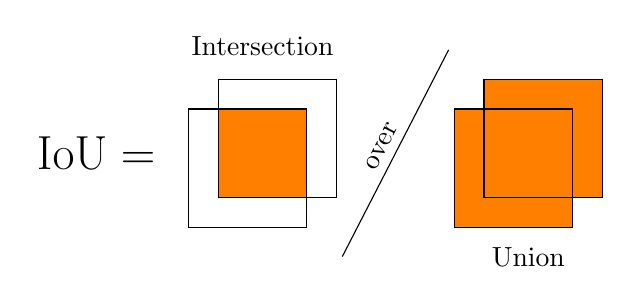
\begin{tikzpicture}[scale=0.75]
  \node[left] at (-0.4, 1.25) {\LARGE $\mathrm{IoU} = $};
  % Intersection illustration
  \begin{scope}
    \clip (0, 0) rectangle (2, 2);
    \fill[orange] (0.5, 0.5) rectangle (2.5, 2.5);
  \end{scope}
  \draw (0, 0) rectangle (2, 2);
  \draw (0.5, 0.5) rectangle (2.5, 2.5);
  \node[above, yshift=0.5em] at (1.25, 2.5) {Intersection};

  % Division sign
  \draw (2.6, -0.5) -- node[auto, sloped] {over} (4.4, 3);

  % Union illustration
  \begin{scope}[shift={(4.5, 0)}]
    \draw[fill=orange] (0, 0) rectangle (2, 2);
    \draw[fill=orange] (0.5, 0.5) rectangle (2.5, 2.5);
    \draw (0, 0) rectangle (2, 2);
    \node[below, yshift=-0.4em] at (1.25, 0) {Union};
  \end{scope}
\end{tikzpicture}

  \caption{%
    Visualization of single-class IoU metric.
  }%
  \label{fig:iou-metric}
\end{figure}

An alternative metric is the dice coefficient, often called the $F_1$ score as well.
The dice coefficient is defined by dividing twice the area of the intersection by the sum of the areas of the two masks:
%
\begin{equation*}
  \mathrm{F_1}
  =
  \frac{%
    2 \cdot |\mathrm{prediction} \cap \mathrm{truth}|
  }{%
    |\mathrm{prediction}| + |\mathrm{truth}|
  }
  =
  \frac{%
    \mathrm{2 \cdot TP}
  }{%
    2 \cdot \mathrm{TP} + \mathrm{FP} + \mathrm{FN}
  }.
\end{equation*}
%
Again we observe that this metric is bounded to the interval $[0, 1]$, with the same interpretation of the endpoints as with the IoU metric.
The visual representation of this metric is given in~\figref{fig:dice-coefficient}.

\begin{figure}[H]
  \centering
  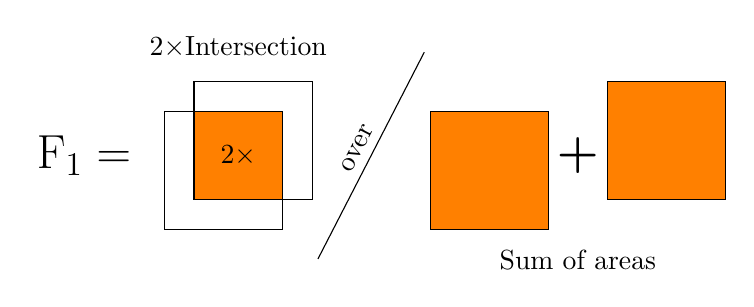
\begin{tikzpicture}[scale=0.75]
  \node[left] at (-0.4, 1.25) {\LARGE $\mathrm{F_1} = $};

  % Intersection illustration
  \begin{scope}
    \clip (0, 0) rectangle (2, 2);
    \fill[orange] (0.5, 0.5) rectangle (2.5, 2.5);
  \end{scope}
  \draw (0, 0) rectangle (2, 2);
  \draw (0.5, 0.5) rectangle (2.5, 2.5);
  \node[above, yshift=0.5em] at (1.25, 2.5) {$2 \times $Intersection};
  \node at (1.25, 1.25) {$2 \times$};

  % Division sign
  \draw (2.6, -0.5) -- node[auto, sloped] {over} (4.4, 3);

  % Union illustration
  \begin{scope}[shift={(4.5, 0)}]
    \draw[fill=orange] (0, 0) rectangle (2, 2);
    \begin{scope}[shift={(2.5, 0)}]
      \draw[fill=orange] (0.5, 0.5) rectangle (2.5, 2.5);
    \end{scope}
    \draw (0, 0) rectangle (2, 2);
    \node[below, yshift=-0.4em] at (2.5, 0) {Sum of areas};
    \node at (2.5, 1.25) {\LARGE \textbf{+}};
  \end{scope}
\end{tikzpicture}

  \caption{%
    Visualization of the single-class dice coefficient metric, also known as the $F_1$ score.
  }%
  \label{fig:dice-coefficient}
\end{figure}

You may have noticed that these two metrics are quite similar; they involve the same quantities, only weighted differently, and are bounded by to the same domain.
In fact, we can construct an exact relationship between these two metrics\footnote{The following relationship and the ensuing inequality bounds were noted by the \textit{Cross Validated Stack Exchange} user \enquote{Willem} here: \url{https://stats.stackexchange.com/a/276144}.}
%
\begin{equation*}
  \frac{%
    \mathrm{IoU}
  }{%
    \mathrm{F_1}
  }
  =
  \frac{1}{2}
  +
  \frac{%
    \mathrm{IoU}
  }{%
    2
  }.
\end{equation*}
%
The two metrics are therefore always positively correlated, as one metric increases or decreases, the other must necessarily follow suit.
A useful insight for how these two metrics actually differ is to observe how the IoU metric is bounded by the $\mathrm{F_1}$ metric:
%
\begin{equation*}
    \frac{%
      \mathrm{F_1}
    }{%
      2
    }
  \leq
    \mathrm{IoU}
  \leq
    \mathrm{F_1}
\end{equation*}
%
The IoU metric is \textit{always} less than or equal to the $\mathrm{F_1}$ metric, but never less than one half its value.
The fraction $\mathrm{IoU} / \mathrm{F_1}$ is equal to 1 whenever the prediction coincides with the ground truth and is equal to $1/2$ whenever there is no overlap at all.
By drawing an analogy to the $p = 1$ (absolute/Manhattan) norm and $p = 2$ (Euclidean) norm, the $\mathrm{IoU}$ metric is somewhat a reflection of the \textit{worst} performance, while the $\mathrm{F_1}$ metric is more a reflection of the \textit{average} performance of a given prediction.


  \topic{Binary cross-entropy and soft dice loss}
  So far all model experiments have been exclusively trained with the \textit{binary cross-entropy} loss function as given in equation~\eqref{eq:binary-cross-entropy}.
While this is the dominant loss function for binary classification tasks, it is still considered a suboptimal surrogate loss function for segmentation evaluation metrics such as the IoU metric.
Alternative loss functions were discussed in~\secref{sec:segmentation-metrics}, the so-called soft loss variants being of greatest interest.
Specifically, the \textit{soft Jaccard loss} given in equation~\eqref{eq:soft-jaccard-loss} and \textit{soft dice loss} given in equation~\eqref{eq:soft-dice-loss} having been theoretically and empirically shown to be efficient surrogate loss functions for the IoU metric.
Three models have been trained and evaluated, the only difference being which loss function that was used during training; binary cross-entropy, soft Jaccard loss, or soft dice loss.
The training procedures of these three models are visualized in \figref{fig:losses-training}.

\begin{figure}[H]
  \centering
  \includegraphics[width=0.66\linewidth]{metrics/lidar_dice_loss+lidar_jaccard_loss+without_rgb-validation-iou}
  \caption{%
    Three U-Net LiDAR models trained with different loss functions.
    Binary cross-entropy model shown in \textcolor{blue}{blue}, soft Jaccard in \textcolor{orange}{orange}, and soft dice shown in \textcolor{green}{green}.
  }%
  \label{fig:losses-training}
\end{figure}

The three models presented in~\figref{fig:losses-training} start out at approximately the same point after one epoch, but the binary cross-entropy model quickly outperforms the two other models when it comes to mean validation IoU.
The soft losses seem to be \emph{worse} surrogate losses for the IoU metric rather than better ones, completely contradicting our prior beliefs.

\begin{figure}[H]
  \centering
  \includegraphics[width=0.49\linewidth,trim={0 0.4cm 0 0.9cm},clip]{metric_correlation/without_rgb+lidar_jaccard_loss+iou}
  \textcolor{gray}{\vrule}
  \includegraphics[width=0.49\linewidth,trim={0 0.4cm 0 0.9cm},clip]{metric_correlation/without_rgb+lidar_dice_loss+iou}
  \caption{%
    Scatter plot showing the correlation between models using different losses during training.
    Both the left and right half of this figure compares model IoU against the binary cross-entropy IoU along the horizontal axis.
    Left figure half shows the soft Jaccard model on the vertical axis, while the right half shows the soft dice loss along the vertical axis.
    See caption of~\figref{fig:correlation-explanation} for detailed figure explanation.
  }
\end{figure}


\newpage
\subsection{State-of-the-Art}%
\label{sec:state-of-the-art}
We will give an overview of the current state of image segmentation.

\begin{itemize}
  \item Deep learning image segmentation overview given here~\cite{segmentation-overview} (\citeyear{segmentation-overview}).
  \item Recent semantic segmentation progress described here~\cite{segmentation-progress} (\citeyear{segmentation-progress}).
  \item Use of fully convolutional networks for semantic segmentation described here~\cite{segmentation-fcnn} (\citeyear{segmentation-fcnn}).
  \item SegNet architecture described here~\cite{segmentation-segnet} (\citeyear{segmentation-segnet}).
  \item U-Net architecture described here~\cite{segmentation-unet} (\citeyear{segmentation-unet}).
  \item Mask R-CNN architecture described here~\cite{segmentation-mask-r-cnn} (\citeyear{segmentation-mask-r-cnn}).
  \item SegCaps architecture described here~\cite{segmentation-segcaps} (\citeyear{segmentation-segcaps}).
  \item Panoptic feature pyramids described here~\cite{segmentation-panoptic-feature-pyramid} (\citeyear{segmentation-panoptic-feature-pyramid}).
\end{itemize}


  \printbibheading[heading=bibintoc,title={Bibliography}]
  \emergencystretch=2em % Insert line breaks correctly on long URLs and titles in bibliography
  \printbibliography[nottype=online,heading=subbibliography,title={Literature}]
  \printbibliography[type=online,heading=subbibliography,title={Online Resources}]
  \section{Image Segmentation --- Central Concepts and Previous Work}
We will now present our numerical experiments, using the theory presented in~\secref{sec:segmentation} and data produced by the pipeline outlined in~\secref{sec:data}.
Specifically the U-Net model architecture is used for segmentation as previously described in~\secref{sec:unet}.
We start by describing the general experimental setup in~\secref{sec:experimental-setup}.
A comparative investigation into the suitability of the different raster data types (aerial photography and/or LiDAR DSMs) for predicting building outlines is presented in~\secref{sec:features}.
In~\secref{sec:technique-experiments} we try to determine if techniques intended to combat overfitting and aid training actually have their intended effect; specifically batch normalization, dropout, and data augmentation.
The different LiDAR normalization methods presented in \algref{alg:local-min-max-scaling} and \algref{alg:metric-normalization} are implemented and compared in~\secref{sec:normalization-experiment}.
Finally, \secref{sec:loss-experiment} presents the empirical efficiency of different surrogate loss functions.


\subsection{Problem Description}%
\label{sec:segmentation-description}
Image recognition seeks to answer three questions for any given image~\cite{image_recognition}:

\begin{enumerate}[nosep]
  \item \textbf{Identification:} Does the image contain any object of interest?
  \item \textbf{Localization:} Where in the image are the objects situated?
  \item \textbf{Classification:} To which categories do the objects belong to?
\end{enumerate}

We will concern ourselves with only one object category (class) at any time, that class being building footprints, and will simplify the following theory accordingly with this simplification in mind.
The localization and classification of objects in a given image can be performed at different granularity levels, as shown in~\figref{fig:segmentation-types}.

\begin{figure}[htb]
  \includegraphics[width=\linewidth,trim={0 4cm 0 3.4cm},clip]{segmentation-types}
  \caption{
    Different granularities for single-class building localization, using the Trondheim 2017 data set.
    Bounding box regression is shown on the left, semantic segmentation in the middle, and instance segmentation on the right.
  }%
  \label{fig:segmentation-types}
\end{figure}
\newpage

\textit{Bounding box regression} concerns itself with finding the smallest possible rectangles which envelopes the objects of interest.
The sides of the rectangles may either by oriented parallel to the axis directions, or rotated in order to attain the smallest possible envelope.
The bounding box will therefore necessarily contain pixels that are not part of the object itself whenever the object shape is not perfectly rectangular.

\textit{Semantic segmentation} rectifies this issue by classifying each pixel in the image independently, i.e. \textit{pixel-wise} classification, producing a so-called classification \textit{mask}.
\textit{Instance segmentation} distinguishes between pixels belonging to different objects of the same class, while \textit{semantic segmentation} does not make this distinction.
Since a bounding box can be directly derived from a semantic segmentation mask, and a semantic segmentation mask can be directly derived from instance segmentation mask; the problem complexity of these tasks are as follows:
%
\begin{equation*}
  \text{Bounding box regression}
  <
  \text{Semantic segmentation}
  <
  \text{Instance segmentation}
\end{equation*}
%
An image of width $W$ and height $H$ consisting of $C$ channels is represented by a $W \times H \times C$ tensor, $X \in \mathbb{R}^{W \times H \times C}$.
This is somewhat simplified, but we will give a more nuanced description in~\secref{sec:raster-data}.
Single-class semantic segmentation can therefore be formalized as constructing a binary predictor $\tilde{f}$ of the form:
%
\begin{equation*}
  \tilde{f}: \mathbb{R}^{W \times H \times C} \rightarrow \mathbb{B}^{W \times H}, \hspace{2em} \mathbb{B} \defeq \{0, 1\}.
\end{equation*}
%
Where $\mathbb{B}^{W \times H}$ denotes a boolean matrix, $1$ indicating that the pixel is part of the object class of interest, and $0$ indicates the opposite.
In practice, however, statistical models will often predict a pixel-wise class \textit{confidence} in the continuous domain $[0, 1]$,
%
\begin{equation*}
  \hat{f}: \mathbb{R}^{W \times H \times C} \rightarrow {[0, 1]}^{W \times H},
\end{equation*}
%
but a binary predictor can be easily constructed by choosing a suitable threshold, $T$, for which to distinguish positive predictions from negative ones
%
\begin{equation*}
  \tilde{f}(X) = \hat{f}(X) > T, \hspace{2em} X \in \mathbb{R}^{W \times H \times C}.
\end{equation*}
%
The choice of the threshold value $T$ will affect the resulting \textit{sensitivity} and \textit{specificity} metrics of the model predictions, metrics which will be explained in the upcoming~\secref{sec:segmentation-metrics}.


\subsection{Convolutional Neural Networks (CNNs)}%
\label{sec:cnn}
  \topic{Convolution}
  As the name implies, a central concept of convolutional neural networks is the so-called \textit{convolution operator}.
Let the \textit{kernel}, $w$, be a $H_k \times W_k$ real matrix, and denote the activation of the previous layer at position $(x, y)$ as $a_{x, y}$.
The \textit{convolution operator}, $\circledast$, is then defined as
%
\begin{align*}
  w \circledast a_{x, y} = \sum_{i} \sum_{j} w_{i, j} ~ a_{x - i, y - j},
  \hspace{3em}
    a_{x, y} \in \mathbb{R},~
    w \in \mathbb{R}^{H_k \times W_k},
\end{align*}
%
where $(i, j)$ spans the index set of the kernel.
The region around $a_{x,y}$ which is involved in the convolution is referred to as the \textit{receptive field}.
We can generate a \textit{filtered image} by moving this receptive field over the entire input image.
The step size used when moving the receptive field is referred to as the \textit{stride size} of the convolution.
This \textit{moving convolution} is illustrated in \figref{fig:convolution}.

\begin{figure}[htb]
  As the name implies, a central concept of convolutional neural networks is the so-called \textit{convolution operator}.
Let the \textit{kernel}, $w$, be a $H_k \times W_k$ real matrix, and denote the activation of the previous layer at position $(x, y)$ as $a_{x, y}$.
The \textit{convolution operator}, $\circledast$, is then defined as
%
\begin{align*}
  w \circledast a_{x, y} = \sum_{i} \sum_{j} w_{i, j} ~ a_{x - i, y - j},
  \hspace{3em}
    a_{x, y} \in \mathbb{R},~
    w \in \mathbb{R}^{H_k \times W_k},
\end{align*}
%
where $(i, j)$ spans the index set of the kernel.
The region around $a_{x,y}$ which is involved in the convolution is referred to as the \textit{receptive field}.
We can generate a \textit{filtered image} by moving this receptive field over the entire input image.
The step size used when moving the receptive field is referred to as the \textit{stride size} of the convolution.
This \textit{moving convolution} is illustrated in \figref{fig:convolution}.

\begin{figure}[htb]
  \input{tikz/convolution.tex}
  \caption{
    Visualization of a kernel convolution with a $3 \times 3$ kernel over an image of size $4 \times 4$ with additional zero-padding and stride size $1$.
    The \textit{receptive field} is shown in \textcolor{orange}{orange}, the respective kernel weights in \textcolor{blue}{blue}, and the resulting convolution output in \textcolor{green}{green}.
    Zero padding of the input image is shown in gray.
  }
  \label{fig:convolution}
\end{figure}

\todo{Finish this section. Some ideas are given below.}

How should we interpret the kernel?
The concept of a \textit{kernel} predates neural networks, and is used in image processing.
Kernel convolution can result in reduction of dimensionality.
The first cause for dimension reduction is that the kernel $(n \times m)$ kernel matrix, with $n, m \geq 1$ can't possibly applied to a $N \times M$ image exactly $N \cdot M$ times. The convolution can't be fit into the image that many times.
We will therefore lose information on the edges of the image after having applied the convolution.
The solution to this problem is to pad the image with zeros.
There are other ways to reduce the dimensionality with convolution.
A $4 \times 4$ kernel with stride $4 \times 4$ will reduce the resolution in both dimensions by four, for instance.

  \caption{
    Visualization of a kernel convolution with a $3 \times 3$ kernel over an image of size $4 \times 4$ with additional zero-padding and stride size $1$.
    The \textit{receptive field} is shown in \textcolor{orange}{orange}, the respective kernel weights in \textcolor{blue}{blue}, and the resulting convolution output in \textcolor{green}{green}.
    Zero padding of the input image is shown in gray.
  }
  \label{fig:convolution}
\end{figure}

\todo{Finish this section. Some ideas are given below.}

How should we interpret the kernel?
The concept of a \textit{kernel} predates neural networks, and is used in image processing.
Kernel convolution can result in reduction of dimensionality.
The first cause for dimension reduction is that the kernel $(n \times m)$ kernel matrix, with $n, m \geq 1$ can't possibly applied to a $N \times M$ image exactly $N \cdot M$ times. The convolution can't be fit into the image that many times.
We will therefore lose information on the edges of the image after having applied the convolution.
The solution to this problem is to pad the image with zeros.
There are other ways to reduce the dimensionality with convolution.
A $4 \times 4$ kernel with stride $4 \times 4$ will reduce the resolution in both dimensions by four, for instance.

  \topic{Activation functions}
  So far we have only explained how a convolutional neural network consists of a set of parametrized linear combinations.
Such networks, if left unaltered, are therefore restricted to only approximating linear functions.
The solution to this predicament is to introduce the concept of \textit{activation functions}, a nonlinear function applied to the output of the convolutional layers.
These activation functions were originally inspired by the neuroscientific understanding of biological neurons~\cite[p.~165]{goodfellow}, but have also been shown to be a theoretical prerequisite of the \textit{universal approximation} property of artificial neural networks~\cite{uat-sigmoid,uat-nonpolynomial}.
The \textit{logistic sigmoid} function, with its deep roots in probability theory, has been a popular choice for activation function in neural networks since the inception of the field~\cite{rosenblatt-perceptron-1958}, and is defined by
%
\begin{equation*}
  \sigma(x) = \frac{1}{1 + e^{-x}} = \frac{e^x}{e^x + 1}.
  \tag{Sigmoid activation function}
\end{equation*}
%
Observe that $\lim_{x \to -\infty} \sigma(x) = 0$ and $\lim_{x \to +\infty} \sigma(x) = 1$, and that the derivative is positive over the entire real number line. This makes it a bounded, differentiable, monotonic function, and is therefore suitable for mapping the weighted output of an artificial neuron in the domain $(-\infty, \infty)$ into the range $(0, 1)$.
This makes it especially suitable for the final layer in neural networks intended for predicting binary 0/1-responses.

Although the sigmoid activation function has a strong biological~\cite{rosenblatt-perceptron-1958} and theoretical~\cite{uat-sigmoid} underpinning, it suffers from the phenomenon of \textit{vanishing gradients} for network architectures consisting of three or more layers, which severely inhibits training.
As an alternative to the sigmoid activation function, the \textit{rectified linear unit} (ReLU) was introduced in a paper~\cite{relu-original-paper} by \citeauthor{relu-original-paper} in year \citeyear{relu-original-paper}.
It is defined as
%
\begin{equation*}
  \mathrm{ReLU}(x) = x^+ = \max(0, x).
  \tag{ReLU activation function}
\end{equation*}
%
The ReLU activation function has become the dominant activation function for use in neural networks in recent years~\cite[p.~438]{relu-popularity} as it has been empirically shown to adapt better to deeper neural networks~\cite{relu-better-than-sigmoid}.

  \topic{Pooling}
  %%%%%%%%%%%%%%%%%%% Local functions %%%%%%%%%%%%%%%%%%%
%% -- Draw marks
\newbox\dumbox% chktex 1
\newcommand{\mymark}[2]{%
  \setbox\dumbox=\hbox{#2}%
  \hbox to \wd\dumbox{\hss% chktex 1
    \tikz[overlay,remember picture,baseline=(#1.base)]{\node (#1) {\box\dumbox};}% chktex 36
    \hss}%
}

%%%%%%%%%%%%%%%%%%% Local functions %%%%%%%%%%%%%%%%%%%

\[
\underbracket[0.6pt][7pt]{
\left[\begin{array}{cccc}
  1 & 8 & \mymark{TL1}{5} & \mymark{TR1}{0} \\
  8 & 11 & \mymark{BL1}{5} & \mymark{BR1}{4} \\
  8 & 17 &               10 & 11               \\
  9 & 12 & 10 & 7 \\
\end{array}\right]
}_{\text{Activations}}
\hspace{0.5em}
\underbracket[0.6pt][7pt]{
\begin{array}{ccc}
    \mymark{TL2}{\phantom{1}} & \phantom{1} & \mymark{TR2}{\phantom{1}}\\
    \phantom{1}  & \mymark{mycenter}{\phantom{1}} &              \phantom{0} \\
    \mymark{BL2}{\phantom{1}} & \phantom{0} & \mymark{BR2}{\phantom{0}}
\end{array}
}_{\text{Pool operation}}
=
\underbracket[0.6pt][7pt]{
\left[\begin{array}{cccccc}
  11 & \mymark{C}{5} \\
  17 & 11 \\
\end{array}\right]
}_{\text{Pooled output}}
\]

\begin{tikzpicture}[overlay, remember picture,
    myedge1/.style={thin, opacity=.3, blue},
    myedge2/.style={thin, opacity=.3, green!40!black}]

  %% Draw boxes
  \draw[orange, fill=orange, fill opacity=.1]   (TL1.north west) rectangle (BR1.south east);
  \draw[blue, fill=blue, fill opacity=.1] (TL2.north west) rectangle (BR2.south east)
    node[midway, opacity=1, color=black] {\Large $\max$};
  \draw[green!60!black, fill=green, fill opacity=.1] (C.north west) rectangle (C.south east);

  %% Draw blue lines
  \draw[myedge1] (TL1.north west) -- (TL2.north west);
  \draw[myedge1] (BL1.south west) -- (BL2.south west);
  \draw[myedge1] (TR1.north east) -- (TR2.north east);
  \draw[myedge1] (BR1.south east) -- (BR2.south east);

  %% Draw green lines
  \draw[myedge2] (TL2.north west) -- (C.north west);
  \draw[myedge2] (BL2.south west) -- (C.south west);
  \draw[myedge2] (TR2.north east) -- (C.north east);
  \draw[myedge2] (BR2.south east) -- (C.south east);
\end{tikzpicture}

  \topic{Batch normalization}
  The reparametrization of earlier layers when training deep neural networks results in a distributional change in the feature layer forwarded to the next layers.
This forces all subsequent layers to adapt to the new \enquote{distributional circumstances}, which in turn impedes the convergence of the optimization.
This phenomenon, referred to as \textit{internal covariate shift}, was first identified in a paper~\cite{batch-normalization} by \citeauthor{batch-normalization}~(\citeyear{batch-normalization}) where they propose a method called \textit{batch normalization} in order to counter this phenomenon.
Suppose we have a layer activation $\vec{a}$ consisting of $d$ dimensions, i.e. $\vec{a} = (a^{(1)}, \ldots, a^{(d)})$.
First we standardize each feature dimension, $k$, independently

\begin{equation*}
  \widehat{a}^{(k)}
  =
  \frac{
    a^{(k)} - \E{a^{(k)}}
  }{
    \sqrt{\Var{a^{(k)}} + \epsilon}
  },
  \tag{Batch standardization}
\end{equation*}

where $\E{\cdot}$ and $\Var{\cdot}$ are respectively sample means and sample variances over the current mini-batch, and $\epsilon$ is added for numerical stability.
The result of this standardization is a feature map where all filters have mean $0$ and variance $1$ for every mini-batch.
The internal covariate shift has been practically eliminated as a result.

This type of normalization alone may not be optimal in all cases, though, and is best explained by constructing a somewhat contrived pathological example.
Assume a set of pooled layer activations $\vec{a}$ to be symmetrically distributed, and assume the subsequent convolution layer to preserve this symmetry.
After standardizing the output, 50\% of the values are expected to be negative, and all of these values will be truncated to $0$ if ReLU is the activation function of choice.
This informational loss may be suboptimal for the given network layer and must be accounted for.
That is to say, $\E{a} =  0$ and $\Var{a}$ may be an unsuitable domain for the given activation function.
For this reason, we introduce two additional trainable parameters for each feature dimension, $\gamma^{(k)}$ and $\beta^{(k)}$, and apply a second normalization step

\begin{equation*}
  y^{(k)} = \gamma^{(k)} \widehat{a}^{(k)} + \beta^{(k)}.
  \tag{Trainable normalization}
\end{equation*}

The intent is to learn the values for the shift, $\beta^{(k)}$, and scaler, $\gamma^{(k)}$, which restores the representative power of the given layer \textit{after} the batch standardization.

  \topic{Dropout}
  Dropout is a regularization technique for neural networks intended to prevent \enquote{complex co-adaption of feature detectors}~\cite{dropout-original-paper}.
In practice this is achieved by randomly omitting hidden nodes from the neural network during each training step; effectively forcing hidden nodes to become less interdependent.
An alternative interpretation of the dropout procedure is that it is a computationally efficient form of model averaging, each dropout permutation being a single model instance.
This technique has been empirically shown to significantly increase the test performance in several different settings.

Although originally intended for use in feedforward neural networks, dropout has been extensively applied in CNN architectures as well~\cite{dropout-cnn}.
Since there are no nodes to be omitted in convolutional architectures, the dropout procedure needs to be adapted in order to be applicable in a CNN setting.
One approach is to introduce a randomly located square mask (\textit{cutout}) to the input image~\cite{dropout-cutout}.
\textit{Stochastic depth dropout} randomly selects entire layers to be dropped, replacing them with identity functions instead~\cite{dropout-stochastic-depth}.
Dropout can also be integrated into max pooling layers, ignoring values at random during the search for the maximum value in the receptive field~\cite{max-pooling-dropout}.
This has become known as \textit{max-pooling dropout} and is illustrated in~\figref{fig:max-pooling-dropout}.

\begin{figure}[htb]
  %%%%%%%%%%%%%%%%%%% Local functions %%%%%%%%%%%%%%%%%%%
%% -- Draw marks
\newbox\dumbox% chktex 1
\newcommand{\mymark}[2]{%
  \setbox\dumbox=\hbox{#2}%
  \hbox to \wd\dumbox{\hss% chktex 1
    \tikz[overlay,remember picture,baseline=(#1.base)]{\node (#1) {\box\dumbox};}% chktex 36
    \hss}%
}
% Used to indicate dropout array indices
\newcommand{\dropout}[1]{{\setlength{\fboxsep}{0pt}\fcolorbox{black}{black}{#1}}}

%%%%%%%%%%%%%%%%%%% Local functions %%%%%%%%%%%%%%%%%%%

\begin{align*}
  \left[\begin{array}{cccc}
    1 & 8 & \mymark{oldTL1}{5} & \mymark{oldTR1}{0} \\
    8 & 11 & \mymark{oldBL1}{5} & \mymark{oldBR1}{4} \\
    8 & 17 &               10 & 11               \\
    9 & \mymark{old}{12} & 10 & 7 \\
  \end{array}\right]
  \hspace{0.5em}
  \begin{array}{ccc}
      \mymark{oldTL2}{\phantom{1}} & \phantom{1} & \mymark{oldTR2}{\phantom{1}}\\
      \phantom{1}  & \mymark{oldmycenter}{\phantom{1}} &              \phantom{0} \\
      \mymark{oldBL2}{\phantom{1}} & \phantom{0} & \mymark{oldBR2}{\phantom{0}}
  \end{array}
  =
  \left[\begin{array}{cccccc}
    11 & \mymark{oldC}{5} \\
    17 & 11 \\
  \end{array}\right]
  \\[2.25em]
  \left[\begin{array}{cccc}
    1 & \mymark{new}{8} & \mymark{TL1}{\dropout{5}} & \mymark{TR1}{0} \\
    \dropout{8} & 11 & \mymark{BL1}{\dropout{5}} & \mymark{BR1}{4} \\
    8 & \dropout{1} &               10 & 11               \\
    \dropout{9} & 12 & 10 & 7 \\
  \end{array}\right]
  \hspace{0.5em}
  \begin{array}{ccc}
      \mymark{TL2}{\phantom{1}} & \phantom{1} & \mymark{TR2}{\phantom{1}}\\
      \phantom{1}  & \mymark{mycenter}{\phantom{1}} &              \phantom{0} \\
      \mymark{BL2}{\phantom{1}} & \phantom{0} & \mymark{BR2}{\phantom{0}}
  \end{array}
  =
  \left[\begin{array}{cccccc}
    11 & \mymark{C}{4} \\
    12 & 11 \\
  \end{array}\right]
\end{align*}

\begin{tikzpicture}[overlay, remember picture,
    myedge1/.style={thin, opacity=.3, blue},
    myedge2/.style={thin, opacity=.3, green!40!black}]

  %% Draw boxes
  \draw[orange, fill=orange, fill opacity=.1]   (TL1.north west) rectangle (BR1.south east);
  \draw[orange, fill=orange, fill opacity=.1]   (oldTL1.north west) rectangle (oldBR1.south east);

  \draw[blue, fill=blue, fill opacity=.1] (TL2.north west) rectangle (BR2.south east)
    node[midway, opacity=1, color=black] {\Large $\max$};
  \draw[blue, fill=blue, fill opacity=.1] (oldTL2.north west) rectangle (oldBR2.south east)
    node[midway, opacity=1, color=black] {\Large $\max$};

  \draw[green!60!black, fill=green, fill opacity=.1] (C.north west) rectangle (C.south east);
  \draw[green!60!black, fill=green, fill opacity=.1] (oldC.north west) rectangle (oldC.south east);

  %% Draw blue lines
  \draw[myedge1] (TL1.north west) -- (TL2.north west);
  \draw[myedge1] (BL1.south west) -- (BL2.south west);
  \draw[myedge1] (TR1.north east) -- (TR2.north east);
  \draw[myedge1] (BR1.south east) -- (BR2.south east);
  \draw[myedge1] (oldTL1.north west) -- (oldTL2.north west);
  \draw[myedge1] (oldBL1.south west) -- (oldBL2.south west);
  \draw[myedge1] (oldTR1.north east) -- (oldTR2.north east);
  \draw[myedge1] (oldBR1.south east) -- (oldBR2.south east);

  %% Draw green lines
  \draw[myedge2] (TL2.north west) -- (C.north west);
  \draw[myedge2] (BL2.south west) -- (C.south west);
  \draw[myedge2] (TR2.north east) -- (C.north east);
  \draw[myedge2] (BR2.south east) -- (C.south east);
  \draw[myedge2] (oldTL2.north west) -- (oldC.north west);
  \draw[myedge2] (oldBL2.south west) -- (oldC.south west);
  \draw[myedge2] (oldTR2.north east) -- (oldC.north east);
  \draw[myedge2] (oldBR2.south east) -- (oldC.south east);

  % Draw arrow from old to new activation matrix
  \draw[->, line width=0.5mm, shorten >= 2mm] (old) ++ (-0.1mm, -4mm) -- node[auto, yshift=1mm] {Dropout} (new.north);
\end{tikzpicture}

  \caption{%
    An example application of \textit{max-pooling dropout} using a receptive field and stride of size $2 \times 2$.
    A dropout probability of $p = 0.25$ has been used.
    Dropped values are shown as black boxes.
  }%
  \label{fig:max-pooling-dropout}
\end{figure}


\subsection{Metrics and Losses}%
\label{sec:segmentation-metrics}
We will now present our numerical experiments, using the theory presented in~\secref{sec:segmentation} and data produced by the pipeline outlined in~\secref{sec:data}.
Specifically the U-Net model architecture is used for segmentation as previously described in~\secref{sec:unet}.
We start by describing the general experimental setup in~\secref{sec:experimental-setup}.
A comparative investigation into the suitability of the different raster data types (aerial photography and/or LiDAR DSMs) for predicting building outlines is presented in~\secref{sec:features}.
In~\secref{sec:technique-experiments} we try to determine if techniques intended to combat overfitting and aid training actually have their intended effect; specifically batch normalization, dropout, and data augmentation.
The different LiDAR normalization methods presented in \algref{alg:local-min-max-scaling} and \algref{alg:metric-normalization} are implemented and compared in~\secref{sec:normalization-experiment}.
Finally, \secref{sec:loss-experiment} presents the empirical efficiency of different surrogate loss functions.

  \topic{Accuracy, sensitivity, and specificity}
  In order to describe segmentation metrics, it is useful to define the following quantities:

\begin{center}
  \fbox{
    \parbox{0.9\linewidth}{
      \begin{description}[font=\sffamily\bfseries, leftmargin=1cm]
        \item[Condition Positive (P)]
          Number of object class pixels in ground truth mask.
        \item[Condition Negative (N)]
          Number of non-object class pixels in ground truth mask.
        \item[True Positive (TP)]
          Number of pixels correctly predicted as being part of object class (correctly identified).
        \item[True Negative (TN)]
          Number of pixels correctly predicted as \textit{not} being part of object class (correctly rejected).
        \item[False Positive (FP)]
          Number of pixel incorrectly predicted as being part of object class (incorrectly identified).
        \item[False Negative (FN)]
          Number of pixel incorrectly predicted as \textit{not} being part of object class (incorrectly rejected).
      \end{description}
    }
  }
\end{center}

False positives (FP) are often knows as \textit{type I errors} in statistics, and false negatives (FN) as \textit{Type II errors}.
The greater the values of TP and TN, the better, and the smaller the values of FP and FN, the better.
A visual representation of these classifications is given in~\figref{fig:confusions}.

\begin{figure}[htb]
  \includegraphics[width=\linewidth]{confusions}
  \caption{
    Binary segmentation problem of size $256 \times 256$.
    The ground truth, a rectangle of size $120 \times 80$ is shown on the left.
    The \enquote{predicted} mask, shown in the middle, is of the same size, but offset by $(-30, -30)$.
    The right figure shows the visual equivalent of a confusion matrix.
    True positives are shown in \textcolor{tp}{dark blue}, true negatives in \textcolor{gray}{light gray}, false positives in \textcolor{fp}{green}, and false negatives in \textcolor{fn}{red}.
  }%
  \label{fig:confusions}
\end{figure}

The simplest metric for semantic segmentation is the \textit{pixel accuracy} metric.
This metric simply reports the percentage of pixels that were correctly classified.
More formally, it can be defined as:

\begin{equation*}
    \textbf{accuracy} = \frac{TP + TN}{TP + TN + FP + FN} = \frac{TP + TN}{P + N}
\end{equation*}

The problem with pixel-wise accuracy metrics is that it does not account for class imbalances.
Consider a problem where 95\% of all pixels are considered to be of class $0$, and the remaining 5\% of class $1$.
If we construct a model which predicts $0$ regardless of the feature inputs provided to the model, the model will achieve a 95\% accuracy score.
This makes pixel-wise accuracy scores difficult to interpret when you do not know the class balance of the respective dataset and the accuracy grouped by class.
This is why it is often replaced by other metrics which takes imbalances into account.
A pair of such metrics is \textit{sensitivity} and \textit{specificity}, formally defined as:

\begin{align*}
    \textbf{sensitivity}
    &=
    \frac{\text{number of true positives}}{\text{number of true positives + number of false negatives}}
    =
    \frac{TP}{TP + FN}
    =
    \frac{TP}{P}
    \\
    \textbf{specificity}
    &=
    \frac{\text{number of true negatives}}{\text{number of true negatives + number of false positives}}
    =
    \frac{TN}{TN + FP}
    =
    \frac{TN}{N}
\end{align*}

The \textit{sensitivity} is therefore a measure of how good the given model prediction was able to identify positives as a relative, fractional value.
Likewise, the \textit{specificity} is a measure of how good the given model prediction was able to identify negatives as a relative, fractional value.


  \topic{Intersection over union and dice coefficient}
  Although the sensitivity and specificity metrics address the issue of class imbalances, they are still \textit{two} distinct metrics that need to be simultaneously inspected in order to get a full performance picture of a given prediction.
We now pose the following problem: \enquote{is it possible to construct a \textit{single} scalar metric which incorporates the idea of sensitivity and specificity?}.
The \textit{intersection over union} (IoU) and \textit{dice coefficient} ($F_1$) are two attempts at solving this problem.

The IoU metric is defined as the area of the intersection between the predicted segmentation mask and the ground truth mask divided by the union of these two masks, or more formally
%
\begin{equation*}
  \mathrm{IoU}
  =
  \frac{%
    |\mathrm{prediction} \cap \mathrm{truth}|
  }{%
    |\mathrm{prediction} \cup \mathrm{truth}|
  }
  =
  \frac{%
    \mathrm{TP}
  }{%
    \mathrm{TP} + \mathrm{FP} + \mathrm{FN}
  }.
\end{equation*}
%
In the case of multiple classes IoU is calculated for each class independently and the result is averaged, known as \textit{mean intersection over union} (MIoU).
MIoU is the most commonly used segmentation metric in research and competitions due to its simplicity and representativeness~\cite{segmentation-overview}.
Notice how the IoU metric is bounded between 0 and 1; $\mathrm{IoU} = 0$ representing a complete \enquote{predictive miss} and $\mathrm{IoU} = 1$ representing a prediction in perfect accordance with the ground truth.
A visualization of this metric is given in \figref{fig:iou-metric} below.

\begin{figure}[H]
  \centering
  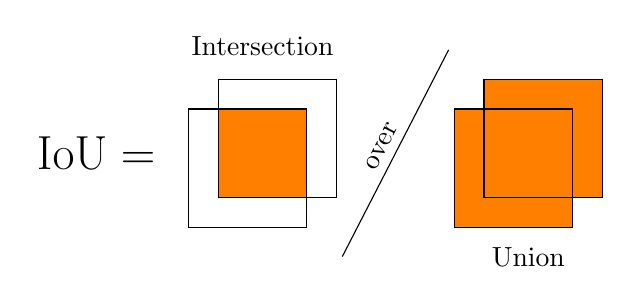
\begin{tikzpicture}[scale=0.75]
  \node[left] at (-0.4, 1.25) {\LARGE $\mathrm{IoU} = $};
  % Intersection illustration
  \begin{scope}
    \clip (0, 0) rectangle (2, 2);
    \fill[orange] (0.5, 0.5) rectangle (2.5, 2.5);
  \end{scope}
  \draw (0, 0) rectangle (2, 2);
  \draw (0.5, 0.5) rectangle (2.5, 2.5);
  \node[above, yshift=0.5em] at (1.25, 2.5) {Intersection};

  % Division sign
  \draw (2.6, -0.5) -- node[auto, sloped] {over} (4.4, 3);

  % Union illustration
  \begin{scope}[shift={(4.5, 0)}]
    \draw[fill=orange] (0, 0) rectangle (2, 2);
    \draw[fill=orange] (0.5, 0.5) rectangle (2.5, 2.5);
    \draw (0, 0) rectangle (2, 2);
    \node[below, yshift=-0.4em] at (1.25, 0) {Union};
  \end{scope}
\end{tikzpicture}

  \caption{%
    Visualization of single-class IoU metric.
  }%
  \label{fig:iou-metric}
\end{figure}

An alternative metric is the dice coefficient, often called the $F_1$ score as well.
The dice coefficient is defined by dividing twice the area of the intersection by the sum of the areas of the two masks:
%
\begin{equation*}
  \mathrm{F_1}
  =
  \frac{%
    2 \cdot |\mathrm{prediction} \cap \mathrm{truth}|
  }{%
    |\mathrm{prediction}| + |\mathrm{truth}|
  }
  =
  \frac{%
    \mathrm{2 \cdot TP}
  }{%
    2 \cdot \mathrm{TP} + \mathrm{FP} + \mathrm{FN}
  }.
\end{equation*}
%
Again we observe that this metric is bounded to the interval $[0, 1]$, with the same interpretation of the endpoints as with the IoU metric.
The visual representation of this metric is given in~\figref{fig:dice-coefficient}.

\begin{figure}[H]
  \centering
  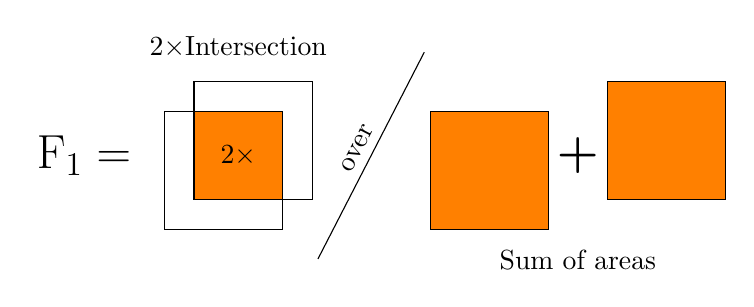
\begin{tikzpicture}[scale=0.75]
  \node[left] at (-0.4, 1.25) {\LARGE $\mathrm{F_1} = $};

  % Intersection illustration
  \begin{scope}
    \clip (0, 0) rectangle (2, 2);
    \fill[orange] (0.5, 0.5) rectangle (2.5, 2.5);
  \end{scope}
  \draw (0, 0) rectangle (2, 2);
  \draw (0.5, 0.5) rectangle (2.5, 2.5);
  \node[above, yshift=0.5em] at (1.25, 2.5) {$2 \times $Intersection};
  \node at (1.25, 1.25) {$2 \times$};

  % Division sign
  \draw (2.6, -0.5) -- node[auto, sloped] {over} (4.4, 3);

  % Union illustration
  \begin{scope}[shift={(4.5, 0)}]
    \draw[fill=orange] (0, 0) rectangle (2, 2);
    \begin{scope}[shift={(2.5, 0)}]
      \draw[fill=orange] (0.5, 0.5) rectangle (2.5, 2.5);
    \end{scope}
    \draw (0, 0) rectangle (2, 2);
    \node[below, yshift=-0.4em] at (2.5, 0) {Sum of areas};
    \node at (2.5, 1.25) {\LARGE \textbf{+}};
  \end{scope}
\end{tikzpicture}

  \caption{%
    Visualization of the single-class dice coefficient metric, also known as the $F_1$ score.
  }%
  \label{fig:dice-coefficient}
\end{figure}

You may have noticed that these two metrics are quite similar; they involve the same quantities, only weighted differently, and are bounded by to the same domain.
In fact, we can construct an exact relationship between these two metrics\footnote{The following relationship and the ensuing inequality bounds were noted by the \textit{Cross Validated Stack Exchange} user \enquote{Willem} here: \url{https://stats.stackexchange.com/a/276144}.}
%
\begin{equation*}
  \frac{%
    \mathrm{IoU}
  }{%
    \mathrm{F_1}
  }
  =
  \frac{1}{2}
  +
  \frac{%
    \mathrm{IoU}
  }{%
    2
  }.
\end{equation*}
%
The two metrics are therefore always positively correlated, as one metric increases or decreases, the other must necessarily follow suit.
A useful insight for how these two metrics actually differ is to observe how the IoU metric is bounded by the $\mathrm{F_1}$ metric:
%
\begin{equation*}
    \frac{%
      \mathrm{F_1}
    }{%
      2
    }
  \leq
    \mathrm{IoU}
  \leq
    \mathrm{F_1}
\end{equation*}
%
The IoU metric is \textit{always} less than or equal to the $\mathrm{F_1}$ metric, but never less than one half its value.
The fraction $\mathrm{IoU} / \mathrm{F_1}$ is equal to 1 whenever the prediction coincides with the ground truth and is equal to $1/2$ whenever there is no overlap at all.
By drawing an analogy to the $p = 1$ (absolute/Manhattan) norm and $p = 2$ (Euclidean) norm, the $\mathrm{IoU}$ metric is somewhat a reflection of the \textit{worst} performance, while the $\mathrm{F_1}$ metric is more a reflection of the \textit{average} performance of a given prediction.


  \topic{Binary cross-entropy and soft dice loss}
  So far all model experiments have been exclusively trained with the \textit{binary cross-entropy} loss function as given in equation~\eqref{eq:binary-cross-entropy}.
While this is the dominant loss function for binary classification tasks, it is still considered a suboptimal surrogate loss function for segmentation evaluation metrics such as the IoU metric.
Alternative loss functions were discussed in~\secref{sec:segmentation-metrics}, the so-called soft loss variants being of greatest interest.
Specifically, the \textit{soft Jaccard loss} given in equation~\eqref{eq:soft-jaccard-loss} and \textit{soft dice loss} given in equation~\eqref{eq:soft-dice-loss} having been theoretically and empirically shown to be efficient surrogate loss functions for the IoU metric.
Three models have been trained and evaluated, the only difference being which loss function that was used during training; binary cross-entropy, soft Jaccard loss, or soft dice loss.
The training procedures of these three models are visualized in \figref{fig:losses-training}.

\begin{figure}[H]
  \centering
  \includegraphics[width=0.66\linewidth]{metrics/lidar_dice_loss+lidar_jaccard_loss+without_rgb-validation-iou}
  \caption{%
    Three U-Net LiDAR models trained with different loss functions.
    Binary cross-entropy model shown in \textcolor{blue}{blue}, soft Jaccard in \textcolor{orange}{orange}, and soft dice shown in \textcolor{green}{green}.
  }%
  \label{fig:losses-training}
\end{figure}

The three models presented in~\figref{fig:losses-training} start out at approximately the same point after one epoch, but the binary cross-entropy model quickly outperforms the two other models when it comes to mean validation IoU.
The soft losses seem to be \emph{worse} surrogate losses for the IoU metric rather than better ones, completely contradicting our prior beliefs.

\begin{figure}[H]
  \centering
  \includegraphics[width=0.49\linewidth,trim={0 0.4cm 0 0.9cm},clip]{metric_correlation/without_rgb+lidar_jaccard_loss+iou}
  \textcolor{gray}{\vrule}
  \includegraphics[width=0.49\linewidth,trim={0 0.4cm 0 0.9cm},clip]{metric_correlation/without_rgb+lidar_dice_loss+iou}
  \caption{%
    Scatter plot showing the correlation between models using different losses during training.
    Both the left and right half of this figure compares model IoU against the binary cross-entropy IoU along the horizontal axis.
    Left figure half shows the soft Jaccard model on the vertical axis, while the right half shows the soft dice loss along the vertical axis.
    See caption of~\figref{fig:correlation-explanation} for detailed figure explanation.
  }
\end{figure}


\newpage
\subsection{State-of-the-Art}%
\label{sec:state-of-the-art}
We will give an overview of the current state of image segmentation.

\begin{itemize}
  \item Deep learning image segmentation overview given here~\cite{segmentation-overview} (\citeyear{segmentation-overview}).
  \item Recent semantic segmentation progress described here~\cite{segmentation-progress} (\citeyear{segmentation-progress}).
  \item Use of fully convolutional networks for semantic segmentation described here~\cite{segmentation-fcnn} (\citeyear{segmentation-fcnn}).
  \item SegNet architecture described here~\cite{segmentation-segnet} (\citeyear{segmentation-segnet}).
  \item U-Net architecture described here~\cite{segmentation-unet} (\citeyear{segmentation-unet}).
  \item Mask R-CNN architecture described here~\cite{segmentation-mask-r-cnn} (\citeyear{segmentation-mask-r-cnn}).
  \item SegCaps architecture described here~\cite{segmentation-segcaps} (\citeyear{segmentation-segcaps}).
  \item Panoptic feature pyramids described here~\cite{segmentation-panoptic-feature-pyramid} (\citeyear{segmentation-panoptic-feature-pyramid}).
\end{itemize}


\end{document}
